\documentclass[twoside]{NSF}

%  \usepackage{amsmath}
\usepackage{amssymb}
\usepackage{rotate}
\let\oldemptyset\emptyset
\let\emptyset\varnothing

\usepackage{ textcomp }
\usepackage[para,online,flushleft]{threeparttable}

\def\changemargin#1#2{\list{}{\rightmargin#2\leftmargin#1}\item[]}
\let\endchangemargin=\endlist 
\usepackage{makecell}
  \usepackage[T1]{fontenc} 
    \usepackage{textcomp} 
   % \usepackage{mathpazo} 
   \usepackage{framed}
      \usepackage{pifont}
\usepackage{adjustbox}
\usepackage{epstopdf}
\epstopdfDeclareGraphicsRule{.gif}{png}{.png}{convert gif:#1 png:\OutputFile}
\AppendGraphicsExtensions{.gif}
\usepackage{rotating}
\usepackage{framed}
\usepackage{colortbl}
\usepackage{wrapfig}
\usepackage{floatflt}
% \usepackage{draftwatermark}
% \SetWatermarkText{Draft}
% \SetWatermarkScale{1}
% \SetWatermarkLightness{.91}

\usepackage{pgfplots}
  
\definecolor{maroon}{cmyk}{0,0.87,0.68,0.32}
\setlength{\parskip}{0.5mm}
\usepackage{indentfirst}
\setlength{\parindent}{0.75cm}

\usepackage{tcolorbox}


\newcommand{\quart}[4]{\begin{picture}(80,4)%1
    {\color{black}\put(#3,2){\circle*{4}}\put(#1,2){\line(1,0){#2}}}\end{picture}}


\usepackage{longtable}
\usepackage{tcolorbox}
\usepackage{caption}
\usepackage{multirow}
\usepackage{comment}
\usepackage{pifont}
\usepackage{array}
\usepackage{enumitem}
\usepackage{hyperref}
\usepackage{fancyhdr}

\newenvironment{myitemize}
{ \begin{itemize}[topsep=0pt,itemsep=0pt,leftmargin=*]
    \setlength{\itemsep}{0pt}
    \setlength{\parskip}{0pt}
    \setlength{\parsep}{0pt}     }
{ \end{itemize}                  } 


%\fancyfoot{}
\pagestyle{fancy}
\fancyfoot{}

\newenvironment{mysmallize}
{ \begin{itemize}[topsep=3pt,itemsep=0pt,leftmargin=10]
    \setlength{\itemsep}{0pt}
    \setlength{\parskip}{0pt}
    \setlength{\parsep}{0pt}     }
{ \end{itemize}                  } 

\usepackage{array}
\usepackage{ragged2e}
\newcolumntype{P}[1]{>{\RaggedRight\hspace{0pt}}p{#1}}



\newenvironment{mynumns}
{ \begin{enumerate}[topsep=0pt,itemsep=0pt,leftmargin=*]
    \setlength{\itemsep}{0pt}
    \setlength{\parskip}{0pt}
    \setlength{\parsep}{0pt}     }
{ \end{enumerate}   }
 
 \definecolor{ao(english)}{rgb}{0.0, 0.5, 0.0}
    

\newcommand{\be}{\begin{mynumns}}
\newcommand{\ee}{\end{mynumns}}

\newcommand{\bi}{\begin{myitemize}}
\newcommand{\ei}{\end{myitemize}}


\newcommand{\bii}{\begin{mysmallize}}
\newcommand{\eii}{\end{mysmallize}}

\newcommand{\tion}[1]{\S\ref{tion:#1}}

\newcommand{\tbl}[1]{Table~\ref{tbl:#1}}
\newcommand{\fig}[1]{Figure~\ref{fig:#1}}

\newcommand{\eq}[1]{Equation~\ref{eq:#1}}

\usepackage[T1]{fontenc} 
\usepackage{textcomp} 
\usepackage{mathpazo} 
   

\definecolor{grey}{gray}{0.9}
\usepackage{xcolor}
% \usepackage{hhline}
% \hyphenation{}

\newcommand{\jnote}[1]{{\color{blue}[JEFF: #1]}} 
\newtheorem{criteria}{Success Criteria}

\usepackage[tikz]{bclogo}
 
\def\checkmark{\tikz\fill[scale=0.4](0,.35) -- (.25,0) -- (1,.7) -- (.25,.15) -- cycle;} 

 
\def\firstcircle{(90:1.75cm) circle (2.5cm)}
\def\secondcircle{(210:1.75cm) circle (2.5cm)}
\def\thirdcircle{(330:1.75cm) circle (2.5cm)}

\newenvironment{eval}[1]%
{\noindent\begin{minipage}[c]{\linewidth}%
\begin{bclogo}[couleur=gray!25,%
                arrondi=0.1, % barre=zigzag,% 
                logo=\bcattention,%
                ombre=true]{~#1}  \begin{criteria}\small}%
{\end{criteria}\end{bclogo}\end{minipage}\vspace{2mm}}

\newcommand{\IT}{{\sffamily {\em \mbox{OMNI-2}}}}

\newcommand{\ACT}[1]{{\sffamily {\bf TASK}$_{#1}$}}

\newcommand{\TITLE}{NSF-CSIRO: 
Can I Trust you, Tomorrow? Building a Predictive and Responsible Foundation for Robust Deep Learning
}

 \usepackage[labelfont=small,font=bf]{caption}
 \captionsetup{font+=sf} 
 
  \usepackage{pifont}

\usepackage{listings}
\usepackage{tcolorbox}
\newtcolorbox{blockquote}{colback=gray!15,boxrule=0.4pt,colframe=gray!15,fonttitle=\bfseries,top=2pt,bottom=2pt}

\usepackage{MnSymbol}% http://ctan.org/pkg/mnsymbol
\usepackage{amsmath}% http://ctan.org/pkg/amsmath
\usepackage{adjustbox}% http://ctan.org/pkg/adjustbox


% \newcommand\hmmax{0}
% \usepackage{bm}


\newcommand*{\skepcon}{\ensuremath{\mathrel{\medvert\mskip-5.7mu\clipbox{1 0 0 0}{$\sim$}}}}



\usepackage{bbm}

\usepackage{changepage}
\usepackage{framed}

% pretty bars
\newcommand{\sbar}[1]{{\color{darkgray}\rule{\dimexpr 0.6cm * #1 / 100}{5pt}\color{lightgray}\rule{\dimexpr 0.6cm * (100 - #1) / 100}{5pt}}}


\makeatletter
\renewenvironment{framed}{%
 \def\FrameCommand##1{\hskip\@totalleftmargin
 \fboxsep=\FrameSep\fbox{##1}
     \hskip-\linewidth \hskip-\@totalleftmargin \hskip\columnwidth}%
 \MakeFramed {\advance\hsize-\width
   \@totalleftmargin\z@ \linewidth\hsize
   \@setminipage}}%
 {\par\unskip\endMakeFramed}
\makeatother

% environment derived from framed.sty: see leftbar environment definition
%\definecolor{formalshade}{rgb}{0.93,0.93,0.93}

\definecolor{formalshade}{HTML}{F9E3DF}
\newcommand{\gray}{\cellcolor{lightgray}}

\newcommand{\floor}[1]{\lfloor #1 \rfloor}


\definecolor{darkblue}{rgb}{0.2, 0.2, 0.2}

\newenvironment{formal}{%
  \def\FrameCommand{%
    \hspace{1pt}%
    {\color{darkblue}\vrule width 2pt}%
    {\color{formalshade}\vrule width 4pt}%
    \colorbox{formalshade}%
  }%
  \MakeFramed{\advance\hsize-\width\FrameRestore}%
  \noindent\hspace{-1pt}% disable indenting first paragraph
  \begin{adjustwidth}{}{7pt}%
  \vspace{1pt}%\vspace{2pt}%
}
{%
  \vspace{3pt}\end{adjustwidth}\endMakeFramed%
}


\begin{document}
\ProjectTitle{\TITLE}
\ProjectAuthor{
%Tim Menzies, NC State
}

%


\begin{nsfsummary} 
\begin{center}
{\bf \TITLE}\\\vspace{1mm}
% Tim Menzies,  IEEE Fellow, NC State
 \end{center}
  
\noindent

\noindent{\bf  OVERVIEW}

We propose a new tool, called \mbox{OMNI-2} that explores a core issue in adversarial attacks
(do different learners return the same decision boundary?)
while also allowing security practitioners and researchers to build more robust models against  white-box   adversarial evasion attacks.

 Many  malware and intrusion detection systems use machine learning-based   detection models. Prior work has shown that such models are susceptible to adversarial evasion attacks where inputs are    crafted by intelligent malicious adversaries  in order make the defender
(e.g. a neural net) misclassify malicious inputs as ``benign''. 
To recognize an adversarial attack,
 a defender must configure a  
learner.  
Using   {\bf {\em multi-objective geometry tricks}}, OMNI-2 can  explore the configuration of a large number of possible    defenders, then cache
100s of {\bf {\em nearly-optimal}}, but {\bf {\em unexpectedly different}}
ones.
By jumping randomly between all those configurations, it is possible to   prevent an adversary from finding,
then exploiting,
patterns in the defenses.
 

\noindent{\bf  INTELLECTUAL  MERIT}

The  success of   OMNI-1   suggests that  prior work made a premature and 
 incorrect conclusion about the value of diversity-based defences (against adversarial learning).  
  Prior work   concluded
    that    different  defending
  learners generate the  same decision boundary
  (the region separating malicious from benign inputs). This is highly
  undesirable since it  mean
   attackers can also learn that structure, {\em even if the attacker does not know
  the learner being used by the defender}.  Yet if this were always so, then OMNI-1 
  would not have worked.  The possibility, to be explored here with OMNI-1, is that  if we jump around a very large range of defense options, we can effectively defend against a wide range of adversarial attacks. 
% This work revisits the value of
% using   ensembles for defending against attackers. The use of such ensembles
%  has its
% defenders and it detractors.
% Here, 
%  we argue here before we can use ensembles to defend against attackers, 
%  it is vital to  change the way we build and use ensembles.  Our ensembles based their  conclusions come from exploring the 
%  {\em far corners of a very large ensemble}, rather than just the center
% of a   small ensemble. 
 



\noindent{\bf BROADER IMPACTS}
 
 
 This work will increase America’s ability for industrial and academic innovators to secure their own
 work.  
This in an important area of research since there  is an increasing reliance of
computational methods in all aspects of our society. 
But the more the international community connects (via software), the more that community
is susceptible to attacks. 
With the growing reliance on information technology, cybercrime is a serious threat to the economy, military and other industrial sectors.
In 2019, the damage cost caused by malware and cybercrime exceeded a trillion dollars. A 2020 study by Accenture reports that cybercrime will cost US \$5.2 trillion over the next five years. Alarming, that cost is growing: the annual average cost to organization of malicious software has grown 29\% in the last year. 



 
 
 In terms of other broader impact,
 this work will inform the curriculum  and lecture notes of the various NC State NSF-funded REUs (research experience for undergraduates) as well as graduate
SE classes (taught by PI Menzies). 
PI  Menzies  will  continue  his  established  tradition  of  graduating  research  students  from  historically under-represented  groups.   
Funds from this work will be used to support students attending the Grace Hopper conference,
and the Richard Tapia Celebration  of Diversity in Computing.

Further,  a (small) portion of this grant would be allocated to support Broadening Participation in Computing (BPC) work. NC  State’s  Computer  Science  department  has  a  strong  record  of  studying research issues related to gender bias,  barriers faced by women, and methods for broadening participation    in  the  context  of  software  engineering.   PI  Menzies  is  a  member  of  his  department’s Broadening Participation Committee (BPC) that actively seeks to:  (a)~Understand hat factors make computer science more (or less) attractive to underrepresented groups; (b)~Educate faculty, staff, and students on how different behaviors effect diversity, quality and inclusiveness; (c)~Increase the percent of students who identify as women; and (d)~Evaluate the success of his department’s BPC team in broadening participating

 

 
 
 
 
 
 

\noindent{\bf KEYWORDS}

Data Science, ML and AI,
Intrusion Detection,
Software

\end{nsfsummary}



\begin{nsfdescription}

\thispagestyle{empty}
 \begin{center}
{\bf \TITLE}\\
{
%Tim Menzies, IEEE Fellow, NC State
}
 \end{center}
\vspace{-3mm}
\noindent
%(In this section, all terms shown in {\bf {\em bold font}} are explained later in this proposal.)

\section{Introduction}  Zhu, Whittle, et al.~\cite{Zhu2022} say that transparency, and the ability to audit complex AI models, are an essential component of 
responsible AI. 
Ben Green~\cite{green2022flaws} notes that many recent policies      require humans review   to assess the decisions from software models.  
When the expertise required for   reviewing is in short supply,     reviews cannot be a human-in-the-loop review of each decision. Rather,   reviews must take the form of some committee
representing {\em stakeholder\footnote{``Stakeholders'' 
are individual or organization having a right, share, claim, or interest in a system or in its possession of characteristics that meet their needs and expectations (ISO/IEC/IEEE 2015~\cite{iso2015systems}).}}
making
{\em occasional audits} (e.g. every week, month, or year). We assume   {\em occasional audits}
since  the  personnel    serving on these audit committees are experts in their field-- which means
that their services are required for  many things  (not just auditing). Hence, 
 audits only occur {\em occasionally}  when those experts can find time
away from their other commitments. 

The problem with   {\em occasional audits} is that while these might occur {\em weekly, monthly, etc}, 
new   hyperparameter optimizers (discussed below) can   update models in {\em minutes, hours, days}.
That means that models change faster than they can be occasionally audited.
(discussed below) which mean it is now becoming   fast to tune deep learning  models.
Does this mean we need to  force humans to continually audit models? Perhaps not.
We propose {\IT} which combines two types of tools to support  occasional  audits {\em as well as} offering some   guarantee
across the space of changes between the audits:  
\bi
\item {\em Audit Tools Type1 (intra-audit):}
  test if a  model is  fair on {\em past cases} by     tunomg the learners  to optimize for multiple stakeholder goals
as well as goals that measure bias and discrimination;
 compare the tuned learner to the original learner;  then recommend a review of   past cases that performed poorly on the original learner, but significantly better on the tuned learner. 
\item {\em Audit Tools Type2 (inter-audit):}
given the tunings from part1, generate {\em worst-case counterfactuals}; i.e. the least change to current data that most reduces performance (as measured by stakeholder goals).   The audit team could    then conclude  that until the model
is extended to cover these worst cases, it must be  policy   never to process  anything like those counterfactuals. 
\ei
{\IT} is novel not just for the {\em Type2} work, but also for the multi-objective nature of {\em Type1}.
Much current work in AI model
robustness focuses just on {\em Type 1}, and only for a single goal such as accuracy (e.g ~\cite{diffenderfer2021winning}).
But in {\IT}, we assume stakeholder care about  a wide variety of domain-specific goals.
We claim that:
\begin{formal}\noindent
 \underline{\bf Stakeholders}  team (i.e. non-technical representatives from  many
 social groups) can \underline{\bf quickly audit}, fault and/or certify   
 \underline{\bf deep learning
models}   via tools which, under-the-hood, using (a)~knowledge distillation, (b)~semi-supervised learning , (c)~landscape
analysis,   and  (d)~multi-objective optimization.\end{formal}
\noindent
 To test this claim, we will perform human studies with {\IT} and 
stakeholders to see how quickly (if at all), they can find seeded faults in ML models.
When evaluating this claim, the term \underline{\em quickly} will become important since 
the experts serving on these audit teams are typically working under strict time constraints
(since they need to get back to their other duties).  

Our pre-experimental belief is that all the   technologies mentioned in our claim are necessary for {\IT}.
Once deep learner {\em distillers} condense the overall search space, we can dividing the model review problem into several simpler task of  reviewing of several small models.
Also,
our (b)~{\em semi-supervised learners}, combined with (c)~{\em landscape analysis}, will allow stakeholders to  ignore   less-informative regions of the models.
Further,
our (d)~{\em multi-objective optimizers} will 
let stakeholders trade off between competing goals. To assess this pre-experimental belief,
we will   conduct ablation
studies~\cite{cohen1995empirical} where each of these (a)(b)(c)(d) will be removed from {\IT}, and the performance of the ablated system will be compared to the whole. 

\section{Background and Motivation}
Green~\cite{green2022flaws}  warns us that {\em
        ..people (including experts) are susceptible to 'automation bias' (involving)  omission errors—failing to take action because the automated system did not provide an alert—and commission error''}. 
        Sadly,
there are   many recent examples   where  ML-models would have benefited from more effective auditing. 
   For example,  it took years to realize that (in)famous
COMPAS  model had an alarming difference in the false alarm rates for black and white defendants~\cite{Chakraborty2020artifact}. 
Facial recognition software   predicting    gender \& age have a much
higher error rate for dark-skinned women~\cite{Skin_Bias}.
  Amazon's   software for same-day delivery   is known to be   biased against black neighborhoods \cite{Amazon_Bias}. 
 Earlier versions of Google Translate  has gender bias
 (e.g. ``She is an engineer, He is a nurse''   translated to  Turkish then
  back to  English gives ``He is an engineer, She is a nurse''~\cite{Caliskan183}). 
Rudin~\cite{rudin2019explaining}, 
Nobel~\cite{noble2018algorithms} and Gebru~\cite{gebru21} list other examples.
When   audit policies routinely miss important problems,  Green remarks that  this   can lead to the reverse of their desired effect  by {\em ``legitimizing the use of   faulty and controversial algorithms without addressing (their fundamental issues''}~\cite{green2022flaws}. 

 


 
\begin{wrapfigure}{r}{2in}
\centerline{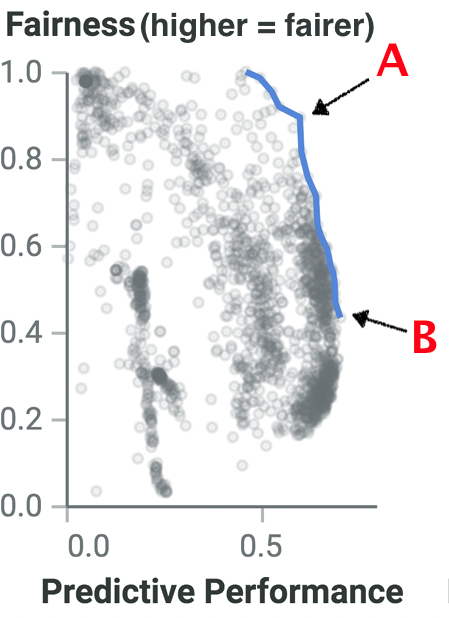
\includegraphics[width=1.5in]{fig/aof.png}}
\caption{Effect of 10,000   tunings
on predicting \underline{\em account opening fraud}.
X-axis= accuracy.
Y-axis= ratio of false positives   men:women.
Learners=
random forest;   regression;   boosted trees; simple decision trees;  a feed-forward NN.
From~\cite{F_Cruz_2021}.}\label{one}\end{wrapfigure}
In many ML models, performance bugs in models learned via machine learning can be addressed via tuning
the control parameters of that model\footnote{For neural networks, those learners can tune many parameters including the
sample shown in 
in Table~\ref{cnn1}.B}
\footnote{For nearest neighbor classification, those algorithms have many tuning options
including (a)~how   to measure
distance; (b)~how many neighbors to consider; (c)~how to combine the influences of those neighbors;
(d)~how (or if) to pre-cluster
the data (in order to optimizer the neighborhood lookup); etc.} 
\footnote{For Random Forests,   those   learners
can tune
(a)~how many $T$ decision trees to build (e.g. $T\in \{10,20,40,80,160\}$); (b)~how many features $F$
to use for each tree (e.g. $F \in{2,4,10,20,
\mathit{sqrt}, \mathit{log2}, \mathit{all}}$);
(c)~what voting measure should be used to poll the whole forest (e.g. {\em majority} or {\em weighted majority}); 
(d)~what impurity measures (e.g. {\em gini} or {\em entropy} or {\em log.loss}); (e)~what is the minimum examples needed to branch a sub-tree
(e.g. {\em min}$\in \{2,5,10,20,50,100\}$; (f)~should branches be {\em binary} or {\em n-arty}.
In all, this gives us
$5*7*2*3*6*2 > 2,500$ different ways, just to configure one   learner in Figure~\ref{one}. }.
For example, see PI Menzies' FSE'20 paper~\cite{Chakraborty_2020} that studied the data used to train a COMPAS-like model. That approach found that false alarm unfairness could be significantly reduced  while  maintaining the same levels of recall on actual recidivism.
 For another example, see 
Figure~\ref{one} comes from Cruz et.al.'s 2021 ICDM paper. 
 %
% In {\em Algorithms of Oppression}, Nobel~\cite{noble2018algorithms} warn us that unfairness 
% cannot be solved merely by looking at   algorithmic details. 
% She argues that ML-software, like any other technology, is   generated in a context that    favors the ruling elite.
% In that view, algorithms
% are as inherently as bad (racist, sexist, extremist, misinforming)
% as anything else selected by their social context.
% Hence, in that view, there is no value in fixing algorithms until we first  fix the society that selects and deploys them. 
%
% While we endorse much of what Nobel says, in this regard,   her viewpoint might be incomplete.
% Just as algorithms designers need to know more the broader
% social issues of their work, so to do social theorists need to know about algorithms.
% For example, 
% consider what the algorithmic perspective can offer the problem of unfairness mitigation.
That figure shows 10,000 different {\em tuning} options on five
machine learners
 As seen in that figure, tunings  drive the
learners from   low to   high accuracies and fairness (measured as the ratio of false positives between men:women).
% Given recent work in {\em hyperparameter optimization} (i.e. automatic tuning algorithms~\cite{lustosa20,lustosa21}),
% it is now possible to efficiently search a large space of options to find (e.g.) the point
% \textcolor{red}{\bf A} in Figure~\ref{one} that offers nearly optimum accuracy and also very good fairness.
Figure~\ref{one} tell is that despite the
external cause of  bias (e.g.   sociological or political), it is still possible to at least partially
mitigate that bias using tuning  algorithms
(as done in~\cite{F_Cruz_2021,Chakraborty_2020}).

There are two issues with tuning: {\em selection preference} and {\em long runtimes}.
 {\em Selection preference},
tuning means making choices about what goals are most desirable.  Consider 
the tuning options shown as points \textcolor{red}{\bf A} 
and
\textcolor{red}{\bf B} in Figure~\ref{one}. If this model was reviewed by a male stakeholder unconcerned with gender
issues, they might select  point \textcolor{red}{\bf A}  since it has higher accuracy. A very different conclusion
might be reached by a female stakeholder who might prefer point \textcolor{red}{\bf B} since that point has nearly highest accuracy, but also very high fairness.  In this proposal, we use multi-objective Pareto frontier techniques
to negotiate trade-offs between the preferences of different stakeholders.

As to {\em long runtimes}, when models are slow to train (e.g. deep learners), it can be impractical
to try 10,000 different tunings (as done in   Figure~\ref{one}). Recently, PI Menzies with his graduate student
Mr. Andre Lustosa, have had   success reducing those runtimes
with semi-supervised learners that explored the tuning options~\cite{lustosa22,lustosa2021preference}.   
SNEAK is a search-based optimization algorithm that inputs thousands of of unevaluated tuning options
(technical note: ``evaluating a tuning option'' means running a learning with those options). 
 SNEAK runs in two passes. In Pass1,   the options are
recursive bi-clustering  by  dividing the 
\begin{wraptable}{r}{4.3in}
\footnotesize
\begin{minipage}{2.5in}
 \hspace{1in} {\bf Table~\ref{cnn1}.A}
\end{minipage}~~\begin{minipage}{1.5in}
  \hspace{.6in} {\bf Table~\ref{cnn1}.B }
\end{minipage}\\~\\
\begin{minipage}{2.5in}
 \begin{tabular}{r|rr}
\rowcolor{blue!10} Optimizer	&Accuracy&	Evaluations\\\hline
Keras Tuner	&89\%&	5\\
Default	&92\%	&0\\
Keras Tuner	&93\%	&50\\
 SNEAK (pass1)&	96\%&	62\\
Keras Tuner&	97\%&	500\\
 SNEAK (pass 2)&	98\%&	130\\
OPTUNA&	98\%	&3500
\end{tabular}
\end{minipage}~~\begin{minipage}{1.5in}
\begin{tabular}{r@{~}|r@{~}|r@{~}|r}
\rowcolor{blue!10}  &	& Batch  	& Dropout  \\ 
\rowcolor{blue!10} &Epochs &	  Size	&   Rate\\\hline
Min &	5&	32	&0\\
Max&	40&	1024&	0.5\\
Step	&1	&32	&0.01\\
\end{tabular}
~\\~\\~\\
\end{minipage} 


 
\caption{For CNN on   Fashion MNIST
(a MNIST-like dataset of 70,000 28x28 labeled fashion images),  Table~\ref{cnn1}.A shows results from hyperparameter optimization of the tuning options of Table~\ref{cnn1}.B. In this study, KERAS~\cite{chollet2015keras} was run three times, with different evalution budgets. OPTUNA~\cite{akiba2019optuna} was executed using its default settings.}\label{cnn1}
\end{wraptable}
tuning options according to each option's
distance to two distant options $X_i,Y_i$ (where distance is measured by a Euclidean measure). SNEAK then reflects over the whole cluster tree to select the split {\em best} that most
reduces the tuning option entropy (from the parent node to its two children). The $X_{\mathit{best}},Y_{\mathit{best}}$   options associated
with that {\em best} split  are then evaluated and SNEAK prunes the sub-tree data associated with the worst of $X_{\mathit{best}},Y_{\mathit{best}}$.
The options surviving Pass1 are   explored in Pass2 by a top-down greedy search that repeats the bi-clustering, but at each stage it just recurses into the better half.
Assuming clustering stops at $\sqrt_N}$ options,  Pass1 and Pass2 explores $N$ tuning options after evaluating just   $O(log_2(N))$ options.

 Table~\ref{cnn1} shows a study    tuning convolutional neural networks where SNEAK's performance was compared
 to a sequenial model-based optimization method (OPTUNA~\cite{akiba2019optuna}) and the standard tuner from Keras~\cite{chollet2015keras}. Note that Pass1 of SNEAK, after 62 options, performed nearly as well as the best
 optimiser, but did so in $\frac{1}{50}$ of the time required for OPTUNA's  3500 evaluations.
 In other   with a dozen SE models, SNEAK found tunings within 1\% to 3\%
of optimum after evaluationg  10 to 100 options while a  prior state-of-the-art
tool~\cite{araujo2017architecture}
(which used stochastic evolutionary   algorithms) needed $1,000$ to $100,000$ questions to get equivalent
results). 
Interestingly, the decisions found by SNEAK out-performed state-of-the-art optimisers such as 
FLASH, HYPEROPT and OPTUNA~\cite{bergstra2015hyperopt,nair18,akiba2019optuna}. We conjecture that those
other optimisers performed worse
since they used a somewhat uninformed
search based on  random mutations.
On the other hand, 
SNEAK did well
 since it reflected on the shape
of the data before deciding what to go next.

XXX bridge para. need to extend sneak for deep elarning.

% That said, rather that patch an unbias algorithm,
% it would be better to eliminated   bias before deployment. How?
% Turning back to Nobel, she notes that if disempowered groups are empowered to participate in the design process, then the odds of generating a biased system are decreased. We hence recommend that AI development models
% are augmented by {\em ocassional audits} where  statkeholder teams
% representing a wide range of  social interests. This proposal discusses some that participation process in the context of   deep learning for CSIRO missions. We will:
% \bi
% \item Define some {\em properties of participation} 
% \item Show how  those {\em properties of
% participation} defeat state-of-the-art hyperparameter tuning optimizers   (in summary, the  search space is too large);
% \item Propose  a new kind of tuning algorithm that is a novel combination of semi-supervised learning, multi-objective optimization, landscape analysis, and deep learner knowledge distillation  (and this new tuner is needed since it divides the search space before exploring it).
% \ei
% To be sure, our approach is mostly algorithmic (so Nobel may not be impressed). But we seek   a ``two-way street'' between what we might call the {\em humanities view} (which is light on CS knowledge) and the {\em computer science view} (which is light on knowledge of the broader social context).
% For example, 
%  consider Timnit Gebru vision of  a future for smart, ethical AI where
%   regulation requires    ``corporations   to show that their technologies are not harmful before they deploy them''~\cite{adams21a}.
% Implementing that requirement, for large institutions, would
% require many things including the automatic algorithms  discussed here.



\section{Alignment with  CSIRO Missions}
Our goal with {\IT} the creation of tools that let any social group appoint some committee to
review a deep learner, and then let that committee have a meaningful interaction with the model (i.e. that group can 
quickly review and  fault,
or  certify, that model). This technology could be used just as well by committees representing different genders or races (in the examples
of our introduction) or committees representing farmers or suburban dwellers, in the examples of Table~\ref{tab:existing}. 

  Table~\ref{tab:existing}  is based on  briefing notes offered to USA researchers on this research proposal,Aug 8, 2022.
  That sessions listed several {\em CSIRO mission related
uses cases} which we
  mapped onto the
the kinds of data sets we are exploring in this area. There are many ways the decisions of these ML-models could make decisions that
unfairly disadvantage different social groups:
\bi
\item
Consider the  suburban dwellers who appear twice times in the {\em Stakeholder} column of Table~\ref{tab:existing}. 
If 
 better water supplies go to   established suburbs with higher rents and house prices, 
 then that would  discriminating against poorer people (who cannot afford to live in those suburbs).
\item
Consider the farmers who appear twice times in the {\em Stakeholder} column of Table~\ref{tab:existing}.     Many farmers 
live geographically distant from government policy makers. Those farmers rarely get to influence the people that make the policy decisions
that effect their lives and livelihood. Hence, their concerns can get overlooked by policy makers.
\ei
The rest of this proposal discusses methods by which  the social groups discussed in the introduction,  or in Table~\ref{tab:existing}, 
can review complex deep learning models.

\begin{table}[!t]
  
 \caption{Deep learning applications applied to   CSIRO missions (https://www.csiro.au/missions), and some key stakeholder concerns. The lesson of this table is that 
    the stakeholder review tools explored in this proposal are a cross-cutting concern applicable to many CSIRO missions.
    Aside: we do not suggest that the list of stakeholders, and their concerns is complete. That said, the current list does
    illustrate how models can make decisions that effect a large group of stakeholders interested in CSIRO's mission}\label{tab:existing}
   
\footnotesize
%fix the table
 \begin{threeparttable}
    \begin{tabular}{p{1in}p{2cm}p{2.6cm}p{3in}}
        \toprule
        \ \textbf{Mission } &  \textbf{Data} & \textbf{Deep Learner}  &  \textbf{Stakeholders} \\
        \midrule
          Drought resilience                 & RecycleNet~\cite{trashnet}                      & ResNet+Attention~\cite{RecycleNet_trash_images} & Farmers (preferring more damns with more water)\\ \cline{4-4}
                                            &                                                   &                                                & Developers wanting less damns (more  real estate space)\\\hline
         Food supply chain supporting        & Traffic prediction dataset~\cite{KaggleTraffic} & GRU~\cite{chung2014empirical}                   & Agribusiness owners (who want to hide predictions, to garner competitive advantage) \\\cline{4-4}
                                            &                                                   &                                                & Farmers (who want access to predictions to plan harvesting and shipping to market) \\  \hline
          AI for health \newlinesurveillance          & Physionet 2017 dataset~\cite{clifford2017af}    & ResNet~\cite{hannun2019cardiologist}           & Doctors (who want to avoid over-treating, least that breeds new strains of resilient bacteria) \\\cline{4-4}
                                              &                                                 &                                                & Potential patients (who, when sick,  demand to be treatment)\\\hline
          AI for flexible\newline  electricity systems & Deep-forecast~\cite{ghaderi2017deepforecast}    & DL-STF\tnote{1}~\cite{ghaderi2017deepforecast} & Power generators (who want to minimize cost of operation from unsold stand-by generation)\\\cline{4-4}
                                               &                                                 &                                               & Suburban dwellers (seeking stand-by power, just in case)\\\hline 
          Water quality\newline forecasting           & Water Quality Data~\cite{zhang2019ssim}         & Dual HeadSSIM~\cite{zhang2021dual}              &  Suburban dwellers (who prefer better sewerage treatment)\\\cline{4-4}  
                                               &                                                 &                                               & State officials (who are reluctant to spend limited budgets funds on capital works)\
        \bottomrule
        
    \end{tabular}
    \begin{tablenotes}
    \item[1] DL-based Spatio-Temporal Forecasting (DL-STF) denotes the spatio-temporal recurrent neural network in~\cite{ghaderi2017deepforecast}.
  \end{tablenotes}
    \end{threeparttable}

\end{table} 

  



\section{US-Australian Team}
The origins of this proposal was a discussion between PI Menzies (USA) and PI Sui (Australia) where we realized that, combining
our   research work, we could   could actual   create  an ethical problem.   This proposal is our  proposed solution
to that ethical problem.

PI Sui is an expert in dividing up the internal state space of a deep learners. Apart from several explorations in knowledge
distillation\footnote{Knowledge distillation transfers knowledge from   large models to  one smaller one~\cite{yim2017gift}.}
and knowledge modulariztion\footnote{The division of one deep learner into several smaller ones~\cite{Tduan2021modularizing}.},
he has also been applying static code analysis methods to deep learners. 
Static code analysis treats programs as a directed graph of connections. By traversing those connections, algorithms
can summarize the important regions in code as well as accumulating the constraints required to reach those regions.
 While the connections
inside a DL may be more plentiful that in source code, those connections are less complex than source code
(since they do not contain loops)
Hence PI Sui found that static code analysis methods  can be used to extract constraints from deep learners.

While PI Sui looks "inside the box", PI Menzies treats the models as black-boxes which he needs to optimize.
A black-box model $f$ converts inputs to outputs using $y=f(x)$. In the general case, models produce multiple outputs
(where $y=\{y_1,y_2,...\}$) so some multi-objective optimizer is required to trade-off between any competing goals.
That trade-off process can be very slow. Returning to Figure~\ref{one}, for example, we see XXX


For example, for optimizing via genetic algorithms, Holland recommends mutating
100 individuals for 100 generations. When applied to a deep learner, that implies running the deep learner for 100*100=10,000
different tuning options~\cite{holland1992genetic}. Given the long training times of these learners, this can be impractical.
Hence PI Menzies explores the use of {\em approximate surrogate models} that (a)~can be built rapidly using just a  few exampples
which (b)~can be used instead of a slow deep learner to evaluate a tuning option. Recently that work has used
semi-supervised learning to implement an approximate landscape analysis which indicates regions of most information~\cite{lustosa21,lustosa22}. By jumping
around the search space only to those most informative regions, PI Menzies' algorithms 
find optimizations that are competitive the 
state-of-the-art   optimizers (e.g.
FLASH, HYPEROPT and OPTUNA~\cite{bergstra11TPE,nair2018finding,akiba2019optuna}) and do so
one to  two orders of magnitude faster.


In summary, PI Sui knows how to explicate structures ``inside the box'' of a deep learner while PI Menzies knows how to reason
``outside the box''. We conjecture that if PI Menzies' algorithms were given access to the internal structures found by PI Sui,
tthen XXXX

XXX add in andre's table here

but what's the problem? well...

% Consider how those missions   benefit from machine learning:
% \bi
% \item
% {\em drought resilience} teams using   learn classifiers that report at-risk crops; 
% \item
% {\em future protein capture}  using
% predictors for  market trends or
% recommender systems that suggest interventions for precision fermentation; 
% \item
% {\em infections disease
% resilience} using anomaly detectors   offeringearly warnings on the arrival of new diseases;
% \item 
% {\em minimising antimicrobial resistance} 
%  preventing super-resistant strains
% by planning minimal antibody interventions. 
% \ei
% Note that all these models have stakeholders with competing goals. 
% To ensure that this work finds relevance for CSIRO missions, we will work with data sets relevant to those missions.  lists the current data sets we are exploring with deep learning.
% That table also  shows how that data relates to CSIRO missions  We envision that as this proposal progresses, we willbe able to access a longer list of data sets that are CSIRO-related.


% \section{Properties of Audits}

% This proposal seeks to support the following {\em properties of audits} that would allow more effectuve auditing. We make the following assumptions:
% \be
% \item
% Such audits are conducted by {\em stakeholder} committees; i.e. teams that champion different   social groups.
% \item
% Stakeholders have different, possible competing {\em goals}; i.e. they must find compromises between  goals.
% \item
% Stakeholders may    not understand the details of AI algorithms; i.e. the audit must be based on their knowledge of the data,
% and not how that data is processed by  AI tools.
% \item
% In our experience, the  personnel recommended to serve on these audit committees are experts in their field-- which means
% that their services are required on multiple tasks (not just auditting). Hence, 
% {\e, audits only occur occasionally| (at  some frequency $T_2$; e.g. weekly, monthly, annually) when those experts can find time
% away from their other commitments.
% \item
% Given recent advances in hyperparameter-optimization (automatic tuning algorithms that adjust the control parameters of a learner\footnote{For nearest neighbor classification, those algorithms have many tuning options
% including (a)~how   to measure
% distance; (b)~how many neighbors to consider; (c)~how to combine the influences of those neighbors;
% (d)~how (or if) to pre-cluster
% the data (in order to optimizer the neighborhood lookup); etc.} 
% \footnote{For Random Forests,   those   learners
% can tune
% (a)~how many $T$ decision trees to build (e.g. $T\in \{10,20,40,80,160\}$); (b)~how many features $F$
% to use for each tree (e.g. $F \in{2,4,10,20,
% \mathit{sqrt}, \mathit{log2}, \mathit{all}}$);
% (c)~what voting measure should be used to poll the whole forest (e.g. {\em majority} or {\em weighted majority}); 
% (d)~what impurity measures (e.g. {\em gini} or {\em entropy} or {\em log.loss}); (e)~what is the minimum examples needed to branch a sub-tree
% (e.g. {\em min}$\in \{2,5,10,20,50,100\}$; (f)~should branches be {\em binary} or {\em n-arty}.
% In all, this gives us
% $5*7*2*3*6*2 > 2,500$ different ways, just to configure this one learner.}), AI models can be
% audited some frequency $T_1 \ll T_2$ (e.g. ever minute, hour, day). That is to say,   
% {\em model updates can be more frequent than audits}. 
% \ei
% These five assumptions lead to two goals listed in the introduction: 
% \bi
% \item[Goal1]: Test if a  model can be fair on {\em past cases}; i.e.  (a)~tune the learners  to optimize for multiple stakeholder goals; (b)~compare the tuned learner to the original learner looking for cases what
%  performed poorly on the original learner, but significantly better on the tuned learner.
% \item[Goal2]: 
% Given the tunings from step1, generate {\em worst-case counterfactuals}; i.e. the least changes to current data that most degrade the optimized
% results.  
% \ei

\subsection{Related Work}

{\textbf{DNN robustness issues.}}
Existing studies mostly focus on data factors affecting the robustness of DNNs. Tripuraneni \textit{et al.} \cite{tripuraneni2021overparameterization} study the high-dimensional asymptotics of random regression under covariate shift; Zhang \textit{et al.} \cite{zhang2020familial} investigate the negative effects of weakly-labelled samples for clustering and proposed a new hybrid representation strategy for familial clustering; Tu \textit{et al.} \cite{tu2020better} found that automatic keyword labelling suffers weakly-labelled issue in bug-fixing commits and recommended to label commits through human+artificial expertise; Shu \textit{et al.} \cite{shu2022omni} argue that well-crafted adversarial samples heavily decrease the identification performance of DNN models and proposed a new Omni solution with multi-model ensemble. 
Some recent studies also explore other factors affecting robustness. For example, Xiao \textit{et al.} \cite{xiao2021nondeterministic} study the impacts of CPU multithreading on DNN systems; 
Pham \textit{et al.} \cite{pham2020problems} explored the performance of identical models with random seeds and nondeterminism-introducing factors under different training runs. These recent approaches provide some insights to understand the impacting factors on DNN robustness. 
In this proposal, we aim to systematically study a wider range of impacts of the data and software implementation and configurations, which will guide our later tasks in on-demand mitigating and repairing robustness issues of the state-of-the-art (SOTA) DNNs. 

{\textbf{Data augmentation and adversarial training.}}
Existing robustness enhancement typically can be done through two main directions: data augmentation and adversarial training.
Data augmentation is usually hinged due to the expensive collection and labelling. To solve this problem, self-supervised or semi-supervised learning methods have been developed to learn feature representations without labelling. 
Among them, the contrastive learning approach SimCLR~\cite{chen2020simple} aims to identify low-dimensional patterns through contrastive learning on two datasets with the same original data and different augmentation methods. 
Unlike SimCLR, MOCO~\cite{he2020momentum} and PIRL~\cite{doersch2015unsupervised} learn the occlusion representations extended from original data to improve precision. 
However, contrastive data augmentation cannot capture the viewpoints of humans and distinguish invariances from the data which are crucial to adversarial training. DebtFree~\cite{tu2022debtfree} applies active learning to discriminate a small amount of representative data by human experts. 
%Familial Clustering~\cite{zhang2019familial} initially takes outlier-aware clustering data and supervised learning methods to automatically classify the unlabelled data.  
Among the existing adversarial training (AT) strategies, GoodFellow \textit{et al}~\cite{goodfellow2015explaining} enhance the generalization of the model through adversarial learning with their proposed simple but efficient method to generate adversarial samples. 
Huang \textit{et al}~\cite{huang2015learning} minimize the classification error against the adversarial samples. 
Zhang \textit{et al.} \cite{zhang2022robustness} propose a CARROT framework to generate adversarial samples through hill climbing. However, these existing methods are still inefficient and/or ineffective in large-scale adversarial training, particularly in the presence of imperfect data and software configurations, which are rarely studied so far. 
In this proposal, we will investigate new active-contrastive-based adversarial training techniques to cope with imperfect data and software configurations in order to mitigate the robustness issues of large-scale DNNs.

{\textbf{Training acceleration.}}
Large neural networks are always resource-intensive and time-consuming in the training stage. Further, these networks cannot be deployed in the inference stage under resource constraint circumstances. Recently, several techniques have been proposed to boost the training efficiency including data quantization and network pruning. 
Data quantization~\cite{wang2020apq} has been deployed to coarsely chop the numerical real numbers to a quantized fixed-bits representation. 
Once For All (OFA)~\cite{cai2020once} supports diverse deployment on various edge devices without an extra training process. 
Joint Search for Network Architecture, Pruning and Quantization Policy (APQ)~\cite{wang2020apq} trains an optimization model by jointly using network architecture pruning and quantization. APQ obtains SOTA efficiency according to the comparisons with the top-ranking methods.
%FlexFlow \cite{Jia2019ParaforDNN} aims to find a fast parallelization optimization strategy to accelerate the training process through the guided random search on the Sample-Operation-Attribute-Parameter (SOAP) space. 
% ByteScheduler \cite{Peng2019DNNaccelerate} accelerates the DNN training process through partitioning and rearranging the tensor transmissions. 
Most of these existing efficiency-driven optimisation (e.g., quantization and pruning) affect the robustness of DNNs. 
In this proposal, we aim to develop a new robustness-preserving model reduction technique to significantly boost the training efficiency while maintaining the model's robustness.

{\textbf{Robustness Certification.}} Robustness~\cite{carlini2017towards} is arguably the most important property to evaluate the reliablity and security of DNNs  ~\cite{NIPS2018shiqi}.
Robustness verification aims to check if any small adversarial  changes to the input can change the output of a DNN. 
In the literature, robustness boundary verification approaches based on formal methods include the exact methods and the approximate methods. 
For the exact method, Reluplex\cite{katz2017reluplex} represents an example of the SMT methods. Tjeng \textit{et al.}~\cite{tjeng2017evaluating} propose a mixed integer programming (MILP) method. These two methods are traditional verification approaches. P{\u{a}}s{\u{a}}reanu \textit{et al.}~\cite{puasuareanu2020probabilistic} propose a method of concolic verification by combining  concrete testing and symbolic execution.
For the approximate method, AI2 \cite{AI2} uses abstract interpretation to certify neural networks. ReluVal\cite{ReluVal} is an interval boundary propagation method, and convex relaxation is a direction such as GeoCert\cite{NEURIPS2019_GeoCert}. 
Exact methods can verify the neural networks precisely but can only verify small-sized DNNs. Approximate methods can approximate the model’s robustness bounds in order to scale the verification for large-size DNNs by sacrificing the verification precision. 
This proposal aims to balance the the exact and approximate methods by proposing a quantitative robustness verification approach based on symbolic execution and constraint solving of DNNs to report not only whether the robustness properties are satisfied, but also indicate where and how many inputs violate them.

{\bf Multi-objective optimization}

{\bf Semi-supervised learning}

{\bf Landscape analysis}

{\bf Knowledge distilation}

% \section{intergration plan}
% \section{Properties}
% unfair is relative

% Cant ask community groups to delve deeply into the algoruthm . e.g. imagine trying to train a bsy lawyer in the  shattered sets of  Vapnik–Chervonenkis theory (and how they apply to SVMs). XXX not going to happen. how to sample i/o pairs.

% Nevertheless, Nobel's warnings do motivate us to ask


% They argue that the root cause of such unfairness are political and social pressures
%  which, for centuries, have systematically blocked dispempowered social groups from influencing the creation and deployment of the systems that control their lives.    
 
% like 

% This issues with  ML-decision models can only get more common.  Many organizations, including the Australian governments CSIRO research group, can use ML-generated models to achieve their goals.
% For example, for CSIRO,  

 


% Consequently, many groups      demand   AI software be    engineered differently in order to   achieve ethical goals~\cite{Gotterbarn} such as 
% the CSRIO~\cite{Zhu2022}, the IEEE \cite{IEEEethics}, the  European Union \cite{EU} and Microsoft \cite{MicrosoftEthics}.
% % This paper discusses how to build software to better address those goals.
% % By  refactoring   recent results in SE,  we can find   data structures and algorithms
% %  that are shared by multiple research results;
% %  and that contribute to multiple ethical goals such as   inclusiveness, transparency, oversight, accountability, privacy, security, reliability, safety, diversity and fairness \cite{ASEGitHub}.
% %Also, there is much recent interest in ethics and software engineering.
% %For example, like us Thomson et al. \cite{THOMSON200185} 
% %stress the   importance of software ethics. 
% %Also, Boland and other researchers \cite{boland2010toward} worked on measuring the trustworthiness of software.
% Entire conference series are now dedicated to this topic: see the ACM FAccT conference    \cite{FAT}   (fairness, accountability, and transparency); 
%  the ``Fairware'' series: https://fairwares.github.io/ (co-organized by co-PI Menzies); and the Software Engineering for Responsible Artificial Intelligence series~\cite{}.

 



% What does it mean to use these models in a {\em responsible} way? Many organizations offer differing definitions on that question. For example,
% if we read the 
% For all these CSIRO missions, and the missions of many other organizations,
% a growing concern in responsible AI
% is {\em procedural justice};
% i.e. procedural justice requires not only fair results but also transparency of the decision-making process such that ones can verify whether the procedure guarantees fairness. O


% \cite{F_Cruz_2021}
% Many methods 
% For the missions of CSIRO,
% and many other
% organizations,
% a cross-cutting concern across many of its  is {\em tuning} the learners in a {\em responsible} way.  
% To understand the
% problems raised by tuning, consider Figure~\ref{one}.
% In this figure,
% hundreds of different tuning options\footnote{
% Examples of tuning parameters include the CNN control parameters of Table{cnn} or, for Figure~\ref{one} the $k,F,p,\epsilon,\mathit{min}$parameters that control the nearest neighbor process.
% After considering $k$-nearest neighbors, such 
% classifiers
% use some kernel function $F$  to sum   the influences of $k$ nearest neighbors (where "near" might be defined using a Minkowski($p$),
% where $p=2$ means "Euclidean). To optimize those distance, calculations, some clustering pre-processor might be applied such as DBSCAN which, in turn has its own tuning parameters such the radius the "local" space $\epsilon$ or the $\mathit{min}$imum allowed size of a cluster.}

% metric controoled by a  o

% once tuning parameter is $k$; i.e. how many neighbors to consider. Once }
% have been applied to a nearest neighbor 
% classification algorithm 

% Why do we say this?
% What is tuning?


% We study tuning since (a)~tuning can dramatically effect the performance of a learner across a range of goals and, (b)~recently, we have had much success with speeding up tuning by an order of magnitude (or via) via landscape analysis.
% That tuning research continues and we foresee
% further speeds up in the near future. Hence we predict that our work, and that of many other resaerchers, will result in highly variable


% tuning
% future speed ups.

% \bi
% \item
% The faster we can tune these learners, the more we can alter their behavior to satisfy different goals.
% \ei

% Responsible-AI means many things~\cite{lu2022softwae}. In this proposal we focus on tools  that {\em let community groups to (a)~review a complex ML model and (b)~certify that it will   will continue to produce ``good'' outputs}
% (where
%  ``good'' is defined by the goals of a particular user group). That is to say,
%  our ML models are ``responsible'' when they  responsive to the needs of those with a stake
%  in the performance of a system.

% There are four main challenges with this goal.
% Firstly, many  goals
% secondly different goals
% thirdly, internal complexity of the models
% fourthly wide space of future tunigns
% fifthly, the alarge earch space
 
%  stakeholders.

% Our recent successes with speeding up tuning by orders of magnitude~\cite{lustosaXX}, described below, show that the behavior of a learner can be altered, very quickly, by 

% By "tunig"


Machine learning models, such as deep neural networks (DNNs), are widely used in many industries and businesses such as supply chain, image  recognition, medical diagnosis and autonomous driving. Significant progress has been made by improving the accuracy of DNN models to boost their productivity. 
However, prior work has shown that high accuracy of a model does not imply high robustness (i.e., consistent performance while being tested on new and future datasets). This is because the input data and the external environment (e.g., software and hardware configurations) for a deployed model are constantly changing. 
Hence, ensuring robustness and trustworthiness of deep learning is not an option but a priority to enhance business and consumer confidence.
The results from our previous work have shown that class imbalance~\cite{shumsr22}, data drifting~\cite{majumder2022methods} and software configurations~\cite{xiao2021nondeterministic} can have significant impacts on the robustness and resilience of a model. Our pilot study in Table~\ref{fig:motivation} also conforms that a variety of factors can yield big performance variances when training AI models, which can  impact many CSIRO's missions~\cite{csiromission}.

Our previous efforts in efficiently finding best models (e.g., Dazzle~\cite{shumsr22} to tackle data imbalance and FLASH~\cite{nair2018finding} to tackle highly configurable systems), have paved the way for the understanding of model robustness, however, they are still insufficient in the presence of dynamically changing data and external environments.
Any trusted and accurate model $f$ trained in the past may not be resilient to accurately predict the unseen future data. 
Given a DNN model $\mathbb{Y} = f_\theta(\mathbb{X})$ which is trained to capture relations between the existing data $\mathbb{X}$ and their labels $\mathbb{Y}$ under a particular model configuration $\theta$, the model $f$ together with its configuration (e.g., hyperparameters) needs to be constantly updated to determine the best possible decision boundary by recognizing new data to maintain its best performance.
Unfortunately, retraining the entire model using new and existing data is very costly, while configuration updates are much cheaper to adjust the model performance.

The previous approaches have been exclusively focusing on either data or model configurations to discover issues in learning models, and the structure of DNNs are often ignored (treated as a blackbox) when pinpointing issues or mitigating variances.
In this proposal, we aim to investigate a holistic approach by providing mitigation choices of robustness issues for end-users. For example, stressing more updating configuration $\theta$ than updating data $\mathbb{X}$ by exploring internal structure of DNN using static symbolic techniques to find the sweet spot for updating model in the presence of dynamically  changing data. 

This proposal will allow AI practitioners and domain experts/researchers to build a predictive and responsible foundation by testing, mitigating, and certifying deep learning models in the presence of dynamically changing data. 
%Our previous approach which treats the model as a black box for searching and mitigating model performance fails to examine the internal structure of DNN models, hence can not provide precise predictive robustness and fine-grained robustness guarantee.
Our approach called \mbox{AIEnvelope} aims to develop (1) a predictive foundation to discover emerging robustness issues by considering both data and model configurations.
(2) mitigation methods to repair robustness issues by supporting less-but-high-quality adversarial data to the best possible configurations.
(3) robustness-preserving model reduction approach to reduce high-cost of robust training and (4) quantitative robustness certification with static symbolic techniques to provide quantitative robustness guarantee.
To explore this type of predictive robust learning and its mitigation techniques, we will need to achieve the following goals. 
%robustness is a negoiatble design construct
%offer choices of variance and 
%These deep learning models in the downstream tasks are so pervasive that we are often unaware of their presence until bugs occur. A single defect or robustness issue can cause fatal errors in safety-critical systems, such as autonomous driving and medical diagnosis.  

%However, many current DNN models are found to have robustness issues, can be unsatisfiable to user expectations, or are susceptible to cybersecurity attacks~\cite{shu2020omni}. Prior work has shown that these AI systems are vulnerable and suffer from reliability issues (e.g., incorrect recognition results), fairness concerns (e.g., bias against underrepresented groups) or lacking user privacy protection (e.g., privacy leakage). 
%This proposal will study the robustness (e.g., accuracy variance) of deep neural network models and their impact on downstream learning tasks. 
%We will investigate mitigation techniques for vulnerable DNNs through generating adversarial data and software configurations using active semi-supervised learning. The repaired DNN model will then be optimized via robustness-preserving optimization to reduce training cost and certified via symbolic verification techniques to provide a quantitative robustness guarantee.

\begin{formal}\noindent
{\bf Goal 1:} Predictive robust deep learning with future data and configurations.\label{goal1}
\end{formal}
\noindent
Robustness is the most noteworthy, well-defined correctness property for reliable and responsible DNNs, i.e., minor modifications to the (future) inputs of DNNs must not alter its outputs. Assuring robustness is critically important to prevent AI systems from environmental perturbations and adversarial attacks.
DNNs are imperfect and existing learning models often yield imprecise or incorrect outputs for real-world applications~\cite{pham2020problems,xiao2021nondeterministic}. 
For example, multiple identical training procedures can generate different models with different accuracy variances in the presence of various factors including imperfect data~\cite{zhang2019familial,menzies2012promise,shu2020omni} (e.g., limited, weakly-labelled and concept-drifting training samples) and variance caused by software implementation and configurations  (e.g., nondeterministic DL layers, and random weight initialization and floating-point imprecision). 
We aim to understand and assess a range of factors that affect the robustness of DNNs and provide guidelines for later mitigation and repair: 

\begin{formal}\noindent
{\bf Goal 2:} Harnessing imperfect data and configuration to improve robustness.
\end{formal}
\noindent
The objective is to investigate robust adversarial training with data and software configuration augmentation techniques through semi-supervised contrastive-active learning. 
Obtaining high-quality training data is the first step to build a robust deep learning model. Based on different robustness impacting factors studied in \textbf{Goal 1}, we will harvest the imperfect training data using a new contrastive-active learning approach to iteratively select unlabelled program samples with distinctive features. This enables automatic or fast semi-automatic labelling, hence significantly reducing
manual labelling costs and improving data quality and quantity. This goal enhances the accuracy and robustness of the underlying model, however, the overhead incurred to the iterative adversarial training can be high if the network structure is large. Improving training efficiency for large-scale real-world data is crucial to obtain a more robust model under the same training time constraint. This leads to our next goal to improve training efficiency:


\begin{figure}[t]
    \centering
    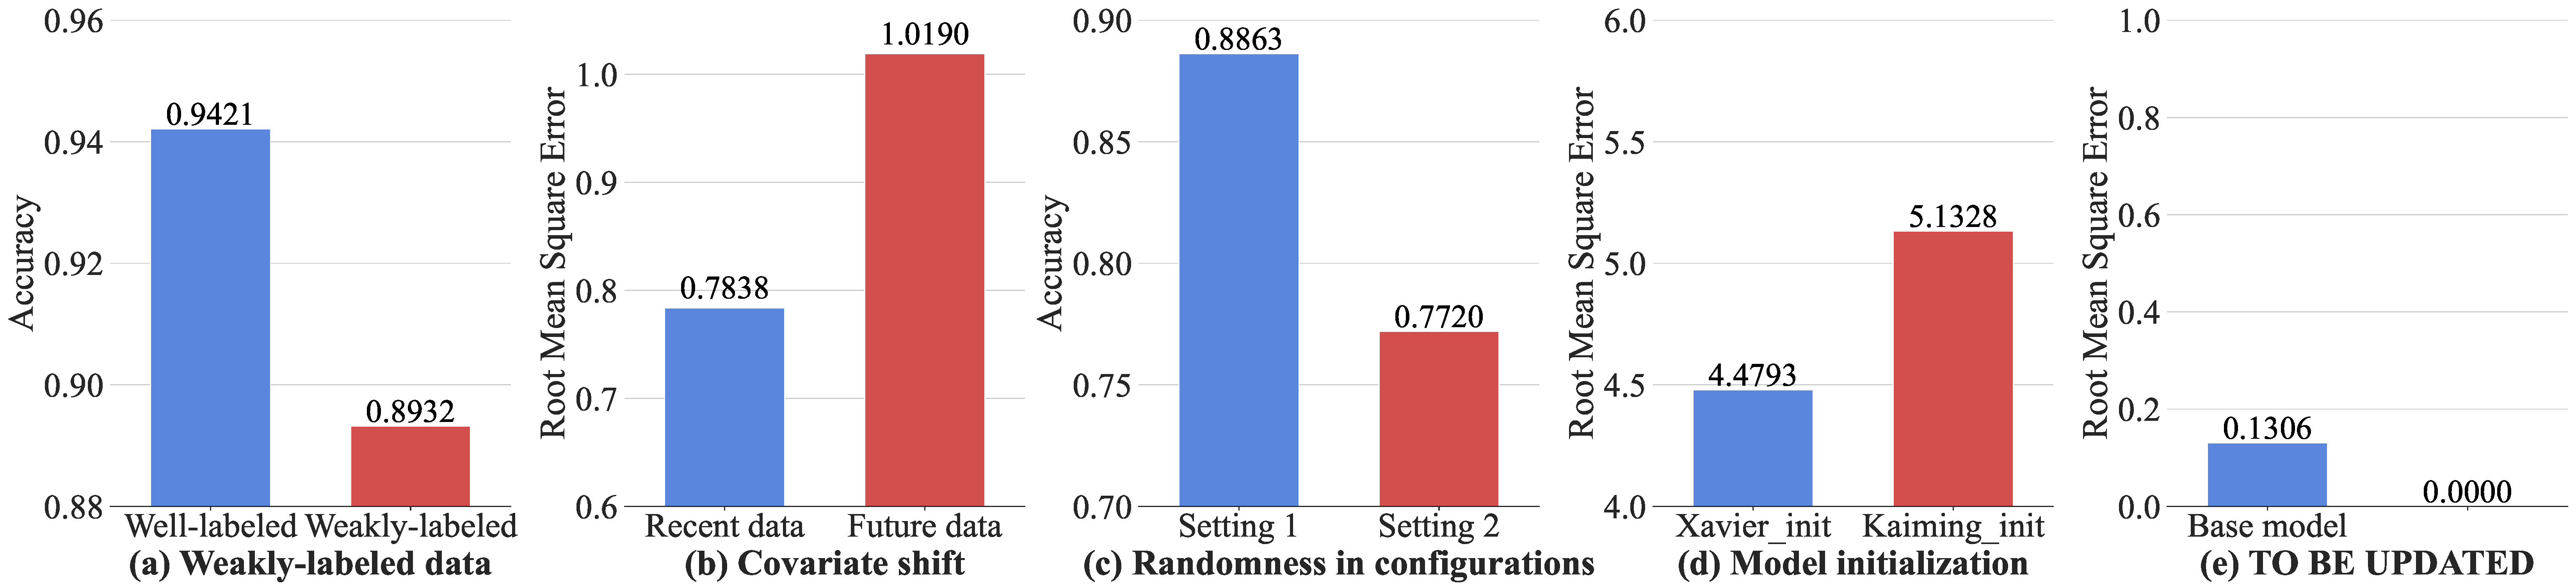
\includegraphics[width=\linewidth]{fig/factors.pdf}
    \caption{Various factors affecting the robustness of deep learning impacting on many of the CSIRO's missions  }
    \label{fig:motivation}
\end{figure}

\noindent
\begin{formal}
{\bf Goal 3:} Model reduction and optimization to  improve training efficiency.
\end{formal}
\noindent
Deep learning models often suffer from redundancy in their network structure, which affects their training efficiency. For example, the over-fitting issue in DNNs~\cite{denil2013predicting} has shown that a large proportion of the configuration parameters are not contributed to the model robustness. 
In this goal, we aim to perform model reduction and optimization to improve training efficiency. Specifically, our novelty lies in robustness-preserved structure transformation to perform network pruning~\cite{han2015learning,luo2017thinet} and  quantize~\cite{ullrich2017soft} through hyperparameter tuning, quantization, parallelism.
The model is reduced and optimized where necessary but preserving the same robustness to boost the adversarial training in \textbf{Goal 2}. Though model reduction (\textbf{Goal 3}) and robustness repair (\textbf{Goal 2}) complement each other, they can be conducted iteratively with one's output as the other's input to continuously improve the overall robustness.
With all that done, we will conduct the final verification to qualitatively certify the underlying DNN model: 
  \noindent
\begin{formal}
{\bf Goal 4:} Quantitative robustness certification of DNN models. 
\end{formal}
\noindent  
Given a repaired and reduced DNN model from \textbf{Goal 2} and \textbf{Goal 3}, our final aim is to conduct precise verification of DNNs using symbolic quantitative certification for the robustness property of the model. 
In the verification of neural networks, a simple yes/no to a verification result about the robustness cannot demonstrate the confidence of the model (e.g., how many perturbed inputs change the model and how much of the deviation of the model has changed). To quantitatively measure and compare the performances of the models by giving in numerous domains would extend the measurement, compared with a threshold deemed with a certain region in a confidence interval. 



%
\section{
Relevance to Responsible AI (material required by solicitation)} 
\subsection{Clear and concise description of the threat model(s)}
\bi
\item
This work assumes that an {\em adversary's goal} is to impact target model’s prediction performance by causing its misclassification in the testing phase, thus 
allowing a malicious payload not being detected.
\item
Also, as to the {\em adversary's knowledge},
we assume a whitebox agent that has access to      knowledge of the defender model as well
as the examples used to train the defender. 
\item
As to the 
{\em adversary’s capability},  we assume adversarial attacks are carried out at the inference time (i.e., testing time), which means the attackers are only able to perturb the immediate inputs, while not be able to manipulate the training dataset. 
\ei
\subsection{Discuss the generalizable theories and research methods that will be developed.} {\bf GOAL5} is
a very general point that speaks to core nature of machine learning.

As to generality of what OMNI-2 can recommend for different data sets, this work will be tested
on a wide range of data sets (including Table~\ref{tbl:securityDataset}, and  other data we   find 
during the course of this research).


Another generalizable result is what this says about  
 ensembles, and their value for  defending against attackers. Ensemble defences has is proponents~\cite{kariyappa2019improving,biggio2010multiple,DBLP:conf/iclr/TramerKPGBM18,smutz2016tree,kantchelian2016evasion} and it detractors~\cite{zhang2020decision,zhang2018gradient,he2017adversarial,DBLP:conf/iclr/TramerKPGBM18,DBLP:journals/corr/PapernotMG16}. 
 We argue here before we can use ensembles to defend against attackers, we need to change the way we build and use ensembles.  
Instead of averaging out multiple conclusions, OMNI  uses conclusions
from a large number of learners {\em all of which are  very
different from each other}\footnote{For an operational definition of ``very different'', see page \pageref{definititions}
of this proposal.}.
That is to say, 
 OMNI's conclusions come from exploring the 
 {\em far corners of a very large ensemble}, rather than just the center
of a   small ensemble. 

\subsection{Discuss the trade-offs and risks involved in the research plan}
See our research plan, below, in
\S\ref{r1}, \S\ref{r2}, \S\ref{r3}, \S\ref{r4} and \S\ref{r5}.

 
\section{Related Work}\label{back}

\subsection{Motivation}

DNNs can be seen as 'programs' composed of training the model parameters (e.g., weights in the networks) from the data. Unlike the hand-written programs by software developers, neural networks lack well-specified requirements and are almost inexplicable, making it challenging to test, analyze and verify their properties (e.g., robustness).

Although DNNs have attained success in real-world complicated tasks such as self-driving systems, malware detection and medical diagnosis, previous research has revealed that a DNN model with high accuracy cannot be guaranteed high  robustness~\cite{ICSE2020W_B_Fairness_Test_Adversarial_Sampling,juuti2019prada,shi2020adaptive,tsipras2018robustness}. This raises reliability and security concerns when applying 
exiting DNN models, especially for mission- and safety-critical scenarios. For example, AdvHat~\cite{AdvHat} uses a simple sticker to fool the face recognition system. Autopilot embedded the DNN models on Tesla vehicles has been involved in around over 200 crashes reported in  2021~\cite{wang2019security}. The vulnerability of DNNs to adversarial attacks has been claimed fatal error in the classification of skin cancer, pneumonia and other diagnoses, a \$250 billion medical industry~\cite{finlayson2019adversarial}. 
There is an increasing demand for responsible AI solutions (e.g., US National AI research and development strategic plan and missions proposed by Australia's CSIRO) because more robust AI models can enhance business and consumer confidence and their productivity by tackling the challenges in a wide variety of domains such as food quality, environmental protection, low carbon industry and etc. For example, responsible AI models can be used to support trusted food supply chain by correctly monitoring and recognizing the quality of food, and more precise recognition for rubbish classification, and even better scheduling of usages of renewable energy~\cite{csiromission}.
%Google searches of the first name of black people are 25\% more than the criminal records search of those of white-identified names~\cite{crawford2016there}. 


Fig.~\ref{fig:motivation} demonstrates a few factors including data and configuration factors that affect the performance of DNNs based on our empirical study.
We briefly describe the following four representative DNNs projects, which yield large performance (accuracy on classification  and regression tasks) variances under four different impacting factors.

\bi
\item {\textbf{(a) Weakly-labelled data}} which contains incomplete or partially labelled training samples can adversely affect the accuracy of the trained DNN models. 
Fig.~\ref{fig:motivation}(a) shows the impacts of weak-labelled data using the widely-recognized RecycleNet~\cite{bircanouglu2018recyclenet} with the TrashNet dataset~\cite {DataTrashNet}, in which the images between plastic bottles and glass bottles are sometimes incorrectly labeled. This  affects the accuracy prediction for the waste classification, which can decrease the classification accuracy by 2.75\% due to weakly label samples in the training set.
%Here, 5\% of samples belonging to plastic and glass are exchanged to simulate the mislabelling process. The simulation results show that the accuracy decreases by 2.75\% due to weak labels.

\item {\textbf{(b) Covariate shift}} which is a distribution  shift among different segments of time periods. This data shifting issue challenges the robustness of the deep learning models like deep Recurrent Neural Network (RNN). 
Fig.~\ref{fig:motivation}(b) shows the large variance of Root Mean Square Error (RMSE) when using two RNN models~\cite{KaggleTraffic} trained with two different temporal data (i.e., 2016.11.1-2017.2.29 and 2017.3.1-2017.6.30) to mitigate the traffic (supply chain) congestion problem. 
%Fig.~\ref{fig:motivation}(b) shows Root Mean Square Error (RMSE) , which are 0.7838 and 1.0190 referred from the recent data (2016.11.1-2017.2.29) and future data (2017.3.1-2017.6.30), which reveals that the unstable prediction performance of the RNN model.
%with the same model configurations

\item {\textbf{(c) Randomness in configurations}} which introduces nondeterminism during the training of DNNs when the stochastic algorithms are used.
%e.g., simulated annealing and stochastic gradient descent. 
Fig.~\ref{fig:motivation}(c) shows the accuracy difference between two training jobs for the DNN-based recognition of  electrocardiograms (ECGs) in cardiac arrhythmia diagnosis~\cite{hannun2019cardiologistlevel,wang2020deep}.  
This critical diagnosis utilizes ResNet~\cite{hannun2019cardiologistlevel} as the default training dataset. We conducted 30 training jobs with random seeds (other settings are the same). The variance of the resulting models can be over 10\%.

\item {\textbf{(d) Model initialization}} which can cause DNN instabilities varied in different initialization methods. We performed the experiments with the same dataset and implementation, except for the weight initialization in the wind speed forecasting project~\cite{ghaderi2017deep}. 
Fig.~\ref{fig:motivation}(d) depicts the RMSEs of the experiments with Kaiming \cite{he2015delving} and Xavier initialization \cite{glorot2010understanding} methods. It can yield a difference of 0.6535 in RMSE.

\ei

\subsection{Related Work}

{\textbf{DNN robustness issues.}}
Existing studies mostly focus on data factors affecting the robustness of DNNs. Tripuraneni \textit{et al.} \cite{tripuraneni2021overparameterization} study the high-dimensional asymptotics of random regression under covariate shift; Zhang \textit{et al.} \cite{zhang2020familial} investigate the negative effects of weakly-labelled samples for clustering and proposed a new hybrid representation strategy for familial clustering; Tu \textit{et al.} \cite{tu2020better} found that automatic keyword labelling suffers weakly-labelled issue in bug-fixing commits and recommended to label commits through human+artificial expertise; Shu \textit{et al.} \cite{shu2022omni} argue that well-crafted adversarial samples heavily decrease the identification performance of DNN models and proposed a new Omni solution with multi-model ensemble. 
Some recent studies also explore other factors affecting robustness. For example, Xiao \textit{et al.} \cite{xiao2021nondeterministic} study the impacts of CPU multithreading on DNN systems; 
Pham \textit{et al.} \cite{pham2020problems} explored the performance of identical models with random seeds and nondeterminism-introducing factors under different training runs. These recent approaches provide some insights to understand the impacting factors on DNN robustness. 
In this proposal, we aim to systematically study a wider range of impacts of the data and software implementation and configurations, which will guide our later tasks in on-demand mitigating and repairing robustness issues of the state-of-the-art (SOTA) DNNs. 

{\textbf{Data augmentation and adversarial training.}}
Existing robustness enhancement typically can be done through two main directions: data augmentation and adversarial training.
Data augmentation is usually hinged due to the expensive collection and labelling. To solve this problem, self-supervised or semi-supervised learning methods have been developed to learn feature representations without labelling. 
Among them, the contrastive learning approach SimCLR~\cite{chen2020simple} aims to identify low-dimensional patterns through contrastive learning on two datasets with the same original data and different augmentation methods. 
Unlike SimCLR, MOCO~\cite{he2020momentum} and PIRL~\cite{doersch2015unsupervised} learn the occlusion representations extended from original data to improve precision. 
However, contrastive data augmentation cannot capture the viewpoints of humans and distinguish invariances from the data which are crucial to adversarial training. DebtFree~\cite{tu2022debtfree} applies active learning to discriminate a small amount of representative data by human experts. 
%Familial Clustering~\cite{zhang2019familial} initially takes outlier-aware clustering data and supervised learning methods to automatically classify the unlabelled data.  
Among the existing adversarial training (AT) strategies, GoodFellow \textit{et al}~\cite{goodfellow2015explaining} enhance the generalization of the model through adversarial learning with their proposed simple but efficient method to generate adversarial samples. 
Huang \textit{et al}~\cite{huang2015learning} minimize the classification error against the adversarial samples. 
Zhang \textit{et al.} \cite{zhang2022robustness} propose a CARROT framework to generate adversarial samples through hill climbing. However, these existing methods are still inefficient and/or ineffective in large-scale adversarial training, particularly in the presence of imperfect data and software configurations, which are rarely studied so far. 
In this proposal, we will investigate new active-contrastive-based adversarial training techniques to cope with imperfect data and software configurations in order to mitigate the robustness issues of large-scale DNNs.

{\textbf{Training acceleration.}}
Large neural networks are always resource-intensive and time-consuming in the training stage. Further, these networks cannot be deployed in the inference stage under resource constraint circumstances. Recently, several techniques have been proposed to boost the training efficiency including data quantization and network pruning. 
Data quantization~\cite{wang2020apq} has been deployed to coarsely chop the numerical real numbers to a quantized fixed-bits representation. 
Once For All (OFA)~\cite{cai2020once} supports diverse deployment on various edge devices without an extra training process. 
Joint Search for Network Architecture, Pruning and Quantization Policy (APQ)~\cite{wang2020apq} trains an optimization model by jointly using network architecture pruning and quantization. APQ obtains SOTA efficiency according to the comparisons with the top-ranking methods.
%FlexFlow \cite{Jia2019ParaforDNN} aims to find a fast parallelization optimization strategy to accelerate the training process through the guided random search on the Sample-Operation-Attribute-Parameter (SOAP) space. 
% ByteScheduler \cite{Peng2019DNNaccelerate} accelerates the DNN training process through partitioning and rearranging the tensor transmissions. 
Most of these existing efficiency-driven optimisation (e.g., quantization and pruning) affect the robustness of DNNs. 
In this proposal, we aim to develop a new robustness-preserving model reduction technique to significantly boost the training efficiency while maintaining the model's robustness.

{\textbf{Robustness Certification.}} Robustness~\cite{carlini2017towards} is arguably the most important property to evaluate the reliablity and security of DNNs  ~\cite{NIPS2018shiqi}.
Robustness verification aims to check if any small adversarial  changes to the input can change the output of a DNN. 
In the literature, robustness boundary verification approaches based on formal methods include the exact methods and the approximate methods. 
For the exact method, Reluplex\cite{katz2017reluplex} represents an example of the SMT methods. Tjeng \textit{et al.}~\cite{tjeng2017evaluating} propose a mixed integer programming (MILP) method. These two methods are traditional verification approaches. P{\u{a}}s{\u{a}}reanu \textit{et al.}~\cite{puasuareanu2020probabilistic} propose a method of concolic verification by combining  concrete testing and symbolic execution.
For the approximate method, AI2 \cite{AI2} uses abstract interpretation to certify neural networks. ReluVal\cite{ReluVal} is an interval boundary propagation method, and convex relaxation is a direction such as GeoCert\cite{NEURIPS2019_GeoCert}. 
Exact methods can verify the neural networks precisely but can only verify small-sized DNNs. Approximate methods can approximate the model’s robustness bounds in order to scale the verification for large-size DNNs by sacrificing the verification precision. 
This proposal aims to balance the the exact and approximate methods by proposing a quantitative robustness verification approach based on symbolic execution and constraint solving of DNNs to report not only whether the robustness properties are satisfied, but also indicate where and how many inputs violate them.









 

 \section{Our Approach}\label{back}
Figure~\ref{fig:figure1} introduces our holistic approach for understanding, repairing and verifying robustness issues in deep neural networks. 
Our proposed framework consists of four major tasks (\textbf{Tasks 1-4}) corresponding to the aforementioned four goals (\textbf{Goals  1-4}). 
Given a DNN model together with its training data and software configurations (e.g., hyperparameters and various training settings), \textbf{Task 1} aims to first study the training factors affecting the model's  robustness e.g., minor perturbations to the data and software configurations of the DNN, which cause to alter its outputs. We aim to capture the correlation between various robustness factors and actual model's behaviour for later mitigating and repairing robustness issues. Subsequently, our \textbf{Task 2} then aims to develop adversarial training to repair robustness issues by harness the imperfect data and various software configurations (studied in Task 1) through semi-supervised active-constrastive learning.

In order to boost efficiency of adversarial training, \textbf{Task 3} aims to develop a robustness-preserving model reduction approach to optimize the DNN structure by pruning the network parts which do not affect the robustness of the DNN. 
Our framework allows \textbf{Tasks 2 and 3} to be performed iteratively, thereby providing increasingly improved robustness and refined model structure for both training accuracy and efficiency.
In \textbf{Task 4}, we will investigate symbolic techniques to qualitatively measure the robustness property of the resulting model from Task 3. Finally, we will certify the robustness of a model \emph{w.r.t}  a lower robust bound (the perturbation distance under which a neural network is proved robust against any allowable perturbation) to  guarantee the model's robustness under an explicit condition. 

\begin{figure}[!t]
    \centering
    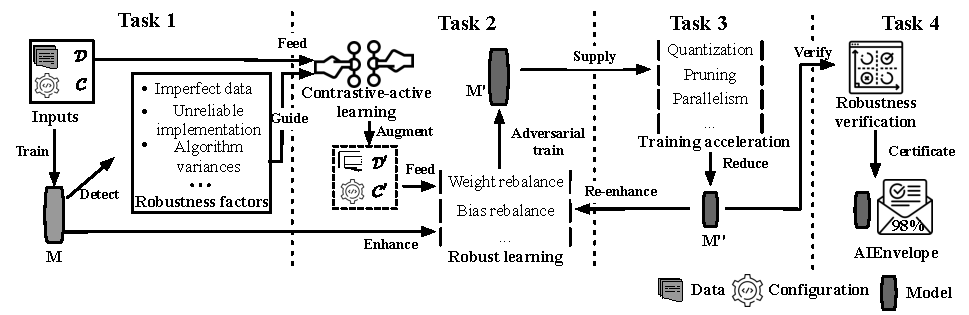
\includegraphics[width=\linewidth]{fig/approach-1.pdf}
    \caption{\mbox{AIEnvelope} framework}
    \label{fig:figure1}
\end{figure}


\section{Research Plan}\label{plan}
Given the aforementioned overall framework, this section details the plan we would like to conduct for each proposed task.
Before we describe each part of our research task (\textbf{Tasks 1-4}), we first formalize the definition of the robustness of DNNs and generalize the four types of problems for robustness measurement, testing and verification. 

{\textbf{DNN robustness formalization.}} A DNN model can be represented as a function $f_{\theta}:\mathbb{X}\rightarrow\mathbb{Y}$, which accepts an input $x\in \mathbb{X} \subseteq \mathbb{R}^n$, and returns an output $y\in \mathbb{Y} \subseteq \mathbb{R}^m$, where $\theta\in\Theta$ denotes the model parameter/architecture configuration, and $\mathbb{X}$ and $\mathbb{Y}$ are the inputs and outputs in the real number domain with $n$ and $m$ dimensions, respectively. A robust DNN is expected to be resilient to a small perturbation on data $(x,y)$ and configuration $\theta$, that is the model (1)  always yields the same output given the same input; (2) is able to identify irrelevant inputs; (3) produces accurate results in the presence of noisy labels, and (4) is stable for accuracy given perturbed model configurations. 
The following formally defines these four aspects for the DNN robustness w.r.t data and configuration.

\bi
\item{\textbf{Data}:} For supervised learning, a DNN model predicts the label of a sample through the trained model which captures the pattern between training data and their pre-defined labels. A trained DNN model $f_{\theta}$ is treated as robust if any input-output relation ($x,y$) always holds under perturbed inputs and outputs.
% input perturbation, irrelevant inputs and noisy labels.

\begin{itemize}[leftmargin=.2in] 

    \item \textbf{Perturbed inputs}: During the training period, perturbed inputs are commonly imposed and can mislead the learning process. In response to the perturbations, a robust DNN can be formalized as:
    \begin{equation}\label{eq1}
    \forall x\in \mathbb{X}, \hat{x}\in \mathbb{X}, \|x-\hat{x}\|_\mathtt{p} < \epsilon \Rightarrow {f_{\theta}(\hat{x})}=y\in \mathbb{Y},
    \end{equation}

where $\hat{x}$ denotes the perturbed inputs under $\mathtt{p}$ normalization with $\epsilon$ distance (the degree of perturbations) to the original input $x$. $\hat{y}$ denotes the corresponding predicted output. 
%To tolerate input perturbations, a robust DNN typically has large decision boundaries. 

    % \item \textbf{Irrelevant inputs}: During the prediction/inference period, there is a common situation of seeking for the classification on a new sample $\hat{x}$ out of the training distribution. In response to this condition, a robust model should give a reliable decision that the predicted result $\hat{y}$ is not classified into any category in $\mathbb{Y}$:
    % \begin{equation}\label{eq2} 
    % \forall \hat{x}\notin \mathbb{X}, \hat{y} = f(\hat{x}) \Rightarrow  \hat{y} \notin \mathbb{Y}.
    % \end{equation}

    \item \textbf{Perturbed outputs}: If the training dataset contains corrupted or imprecise labels ($\hat{y}$) under $\delta$ distance to the human-desired labels ($y$) and deviated by $\tau$ times to the inference result, a robust model $f_{\theta}$ can still output the correct $y$:
%clustering center
    \begin{equation} \label{eq3} 
    \forall (x, \hat{y})\in( \mathbb{X}, \mathbb{Y}), \hat{y} = \tau \cdot f_{\theta}(x), \  \|f_{\theta}(x)-\hat{y}\|_\mathtt{p} < \delta  \Rightarrow f_{\theta}(x) = y\in \mathbb{Y}.
    \end{equation}
\end{itemize}

\item{\textbf{Configurations}:} In addition to data factors, the training variance from configurations (e.g., model initialization and hyperparameters) is another reason for the robustness issues of DNNs. A trained DNN is said to be robust if prediction variance is less susceptible to configuration perturbations:
    \begin{equation}\label{eq4}  
   \forall  x\in \mathbb{X}, \theta \in \Theta, \hat{\theta} \in \Theta, \|\theta-\hat{\theta}\|_\mathtt{p} < \eta \Rightarrow f_{\theta}(x)=f_{\hat{\theta}}(x)=y\in \mathbb{Y},
    \end{equation}
where $\hat{\theta}$ denotes the configuration under $\mathtt{p}$ normalization with $\eta$ distance (configuration differences) to the configuration $\theta$.



\ei

 \subsection{Task 1: Study and understand the robustness factors of deep neural networks.}\label{4.1}


Previous efforts have focused on the data impacts of DNN robustness, however, fewer studies towards a holistic understanding of a wider range of configurations (e.g., model parameters and structure) and their coalesced effects with imperfect data for DNN robustness. 
In this task, we aim to systematically analyze the influence of each factor and their combinations (composition effects) on the robustness of DNN model in a range of downstream domains including image classification, video motion recognition, and medical diagnosis in Table~\ref{tab:existing}. 

In Table~\ref{tab:factors}, we consider the perturbation surface (i.e., data ($F_D$) and configuration ($F_C$)) and their specific modification targets, i.e., input, output, model parameter and structure. 
For each factor $F_i \in $ \{ $F_1$, $\dots$, $F_N$ \}, 
it has a set $T_{F_i}$ of modifications, including changing inputs, outputs and configurations to different pre-defined values. 
We use $\omega \subseteq T_{F_1}\dots\times T_{F_i}\dots \times T_{F_N}$ to represent a \emph{perturbation strategy}, which is a subset of all modifications given all factors combined. Hence we can train and produce different DNN models (e.g., $\mathcal{M}$) based on individual strategies (e.g., $\omega$) 

\begin{equation}
\label{eq:perturb_train}
    \mathcal{M}=train(\hat{\mathbb{X}},\hat{\mathbb{Y}}, \hat{\Theta}), \quad  s.t. \ \
    \hat{\mathbb{X}},\hat{\mathbb{Y}}, \hat{\Theta} = perturb_{\omega}(\mathbb{X},\mathbb{Y},\Theta),
\end{equation}
where $\hat{\mathbb{X}}, \hat{\mathbb{Y}}, \hat{\Theta}$ are modified inputs, outputs and configurations based on the strategy $\omega$.

\begin{wraptable}{r}{9.7cm}
\vspace{-5mm}
     \caption{\footnotesize Robustness affecting factors}
     \footnotesize
    \begin{tabular}{llc}
    \toprule
        \textbf{Surface} & \textbf{Factor} & \textbf{Modification Target}\\\midrule
        \multirow{3}{*}[-0.5\dimexpr \aboverulesep + \belowrulesep + \cmidrulewidth]{Data ($F_D$)} & $F_1$ Adversarial attack &  Input $\mathbb{X}$ \\\cline{2-3}
                        &$F_2$ Label flipping attack & \multirow{2}{*}[-0.5\dimexpr \aboverulesep + \belowrulesep + \cmidrulewidth]{Output $\mathbb{Y}$} \\ 
                        &$F_3$ Label noise injection  \\ \midrule
        \multirow{4}{*}[-0.5\dimexpr \aboverulesep + \belowrulesep + \cmidrulewidth]{ Configuration ($F_C$)}& $F_4$ Weight perturbation   & \multirow{4}{*}{Model $\Theta$ } \\ 
                       & $F_5$ Bias perturbation  &        \\
                       & $F_6$ Conv layer modification\tnote{1}&  \\
                       & $F_7$ FC layer modification\tnote{2} & \\
                        $\ldots$ &$\ldots$ &$\ldots$ \\
   \bottomrule
    \end{tabular}
    \label{tab:factors}
\end{wraptable}

Given $N$ factors with each having $T$ modifications, we will have combinations of $2^{T*N}$ perturbation strategies to exercise and test the robustness of a DNN model during its training. This search space is huge when trying to determine which strategy is more effective to degrade the robustness of the model, while the exhaustive enumeration in this search space by using the traditional methods (e.g. grid search) is time-consuming and labor-intensive. 
To alleviate the combinatorial explosion problem, we will investigate a differential evolution (\textbf{DE}) approach to capture cumulative confidence decision boundary (\textbf{C-CDD}) by selectively and iteratively searching the top-$Q$ most influential perturbation strategies.

\begin{wrapfigure}{l}{9.5cm}
    \centering
        \vspace{-3mm}
    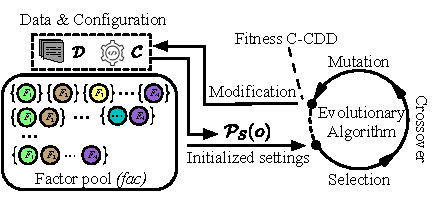
\includegraphics[scale=1]{fig/Task1.pdf}
    \vspace{-3mm}
    \caption{\footnotesize Differential Evolution Configuration}
    \label{fig:task1frame}
\end{wrapfigure}


\textbf{C-CDD.} Deep learning aims to predict the class of a sample $x\in\mathbb{X}$ by estimating the probability $p_{\mathcal{M}}(y\ |\ x)$ on each class by a model $\mathcal{M}$ which is trained based on Equation~\ref{eq:perturb_train}. \emph{Cumulative confidence decision boundary} (C-CDD) as defined in Equation~\ref{eq:cumlativeCDD} is used to estimate $\mathcal{M}$'s robustness by measuring the confidence of all predicted samples in $\mathbb{X}$. 
C-CDD reflects the relative distance of the inputs from the decision boundary to the human desired classes. 
A lower C-CDD score indicates that the model potentially has higher uncertainties (less robust) in its predictions. 
%To further shrink the search space, smaller modifications from fewer factors are always preferable if it has a similar C-CDD score as that of more modifications. 

\begin{equation}\label{eq:cumlativeCDD}
  \text{C-CDD} (\mathbb{X}, \mathcal{M})=  \mathbb{E}_{x\in\mathbb{X}}(p_{\mathcal{M}}(i\ |\ x)-p_{\mathcal{M}}(j\ |\ x)),
\end{equation}
where $\mathbb{E}$ denotes the expectation operation, $i$ denotes the human desired class and $j$ is the predicted class with the maximum prediction probability. 


\textbf{DE.} \emph{differential evolution} (DE)~\cite{DBLP:conf/ijcai/AwadMH21} is a fast global optimization algorithm to guide the search of the optimal perturbation strategies that perturb the DNN model effectively. 
Initially, we randomly generate a population of $Q$ strategies as the first generation. 
$\omega_i^g$ denotes $i$-th ($1 < i \leq Q$) strategy in the $g$-th generation. 
DE aims to optimize and mutate the $Q$ strategies in multiple generations in an evolutionary manner with a gradually reduced C-CDD score until a generation that produces the model has the lowest or a pre-defined C-CDD score. 


% \begin{figure}[!h]
%     \centering
%     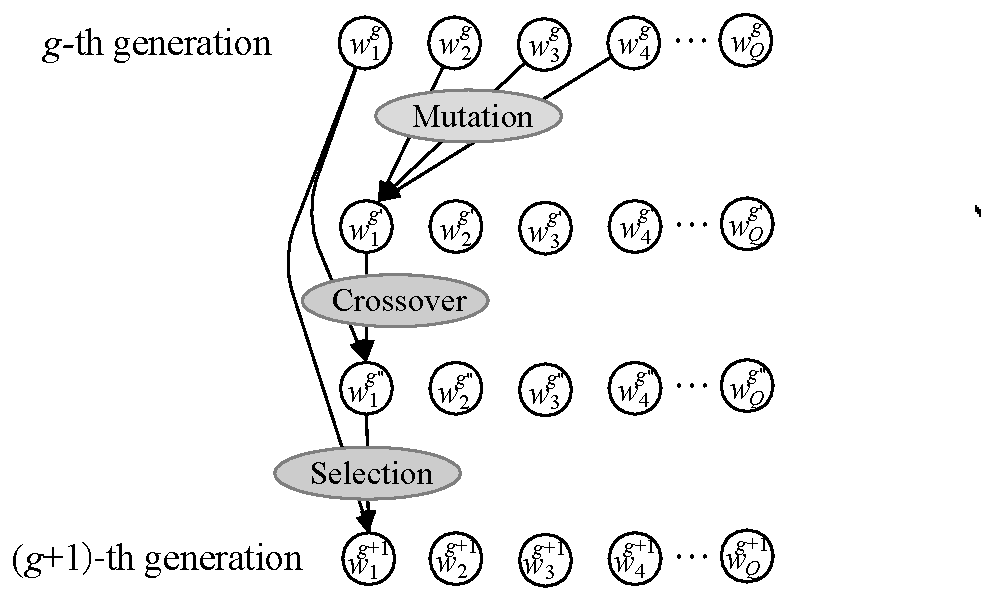
\includegraphics[width=9cm]{fig/DE.pdf}
%     \caption{population generation in DE.}
%     \label{fig:goal2}
% \end{figure}

For $\forall \omega_i^{g+1}$ in $(g+1)$-th generation, DE conducts the following four steps in order: 
\begin{enumerate}
    \item Generate. Three strategies $\omega_{r_1}^g$, $\omega_{r_2}^g$, $\omega_{r_3}^g$ are randomly selected from the population in $g$-th generation. The generated indexes must be distinct from each other and also different from the strategy index $i$ in $(g+1)$-th generation, i.e., $r_1 \neq r_2 \neq r_3 \neq i$.
    \item Mutate. The strategy for the $(g+1)$-th generation in the population is mutated by $\omega_i^{g+1} = \omega_{r_1}^g + \epsilon (\omega_{r_2}^g-\omega_{r_3}^g)$, where $\omega_{r_1}^g$, $\omega_{r_2}^g$, $\omega_{r_3}^g$ are generated from Step 1, and $\epsilon\in(0,1]$ denotes a scaling coefficient.
    \item Crossover. The strategy can be treated as a $K$-length vector that contains a sequence of  modification methods. Let $\omega_i^g[j]$ denote the $j$-th ($1\leq j \leq K$) modification in the perturbation strategy. 
    The crossover follows a random probability value from the uniform distribution, i.e., $r_i^{g}[j] \sim U(0,1)$. The $(g+1)$-th generation of each particular modification in the perturbation strategy can be obtained as: 
    \begin{equation}
    \omega_i^{g+1}[j] = \left\{ 
     \begin{array}{ll}
           \omega_i^{g}[j], & if\ r_i^{g+1}[j] < p_r \\ 
           \omega_i^{g+1}[j],& otherwise
     \end{array}
     \right. 
    \end{equation}
    Here, $p_r$ is a user-specified replacement rate (e.g.,  $0.9$).
    
    \item Select. For each newly generated strategy $\omega_i^{g+1}$, we produce a different DNN model by Equation~\eqref{eq:perturb_train} and select between $\omega_i^{g}$ and $\omega_i^{g+1}$ based on a lower C-CDD score calculated by Equation~\eqref{eq:cumlativeCDD}. 

\end{enumerate}

Given the top-$Q$ strategies and their trained models produced by DE, we will exploit effective methods of robustness enhancement in the \textbf{Task 2}.

\subsection{Task 2: Harnessing imperfect data and configuration to improve robustness.}

Regarding the identified robustness issues found in \textbf{Task 1}, we plan to improve the robustness of the trained model $\mathcal{M}$ on the top-$Q$ perturbation strategies via contrastive robust learning (CRL). In this project, CRL aims to learn the robust representation by contrasting similar (positive) and dissimilar (negative) objects instead of learning to recognize them individually. We intend to extend the contrastive learning paradigm into three imperfect DNN scenarios: perturbed inputs, perturbed outputs, and configuration variance. 

Regarding the scenarios with different perturbation strategies, the given target data are applied to its fitted contrastive loss: 
(1) Adversarial loss is addressed in the perturbed inputs scenario that the contrastive pair is the target inputs and their following perturbed inputs which can be viewed as positive pairs; 
(2) Label-flipping loss is computed on the variations of the noisy labels to reduce the effects of imprecise labels, by which the ground-truth labels and noisy labels can be viewed as negative pairs; 
(3) Configuration loss is utilized to update our target model to be trained dissimilar to the perturbed model which is proven to be less robust.
Furthermore, we propose a $mixture-loss$ for CRL, which is a concise loss function to enhance the robustness of the model in addressing the three scenarios together.

\begin{figure}[!h]
    \centering
    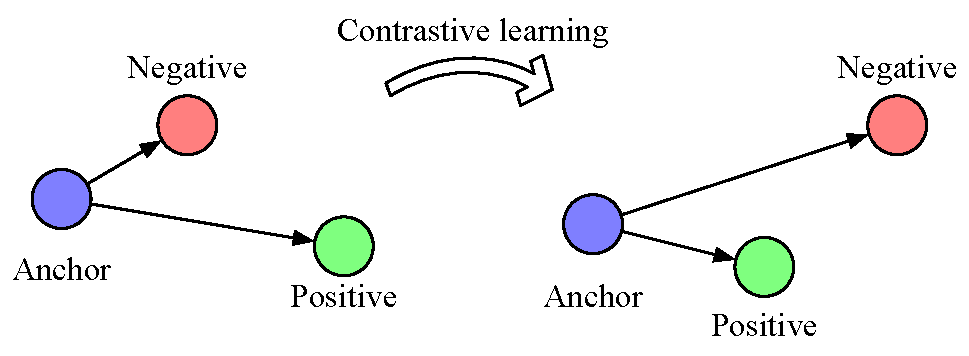
\includegraphics[width=9cm]{fig/contra.pdf}
    \caption{Contrastive learning}
    \label{fig:goal2}
\end{figure}

\textbf{Contrastive loss} Following the above definition of the model $f_{\Theta}: \mathbb{X} \rightarrow \mathbb{Y}$, the loss function quantifies the differences between the expected outcome and the model produced one. Contrastive loss obtains the outputs of the network for the positive (similar) examples of the same class, which is expected to be minimized, and contrasts that with the distance to negative (dissimilar) examples, which is expected to be maximized. Formally, the contrastive loss is present for the similar and dissimilar cases in Equation~\eqref{eq:contra}:
\begin{equation}\label{eq:contra}
    \mathcal{L}_{ct}(x_i,x_j) = \left\{\begin{matrix}
                          \|f_{\theta}(x_i)-f_{\theta}(x_j)\|_{\mathtt{p}} + \gamma,    & ct=+ \\
                          - \|f_{\theta}(x_i)-f_{\theta}(x_j)\|_{\mathtt{p}} + \gamma,  & ct=-
    \end{matrix}\right.
\end{equation}
where $\gamma$ is a hyper-parameter that is configured for the offset to the distances of a positive ($ct=+$) or negative ($ct=-$) pair, and the $x_j$ and $x_i$ are sampled from or generated by the strategies in $\mathbb{X}$ or $\hat{\mathbb{X}}$. 

\textbf{Adversarial loss} Given one target training input (anchor input) $x\in\mathbb{X}$, we can generate the corresponding perturbed input $\hat{x} \in \hat{\mathbb{X}}$ via the perturbation strategy $\omega$. 
Following the Equation~\eqref{eq:contra}, in Equation~\eqref{eq:adv}, we set every original input and its perturbed one as a positive pair ($x_i,\hat{x_i}$); we set original data from dissimilar classes ($x_i,x_j$), the original data from perturbed dissimilar classes ($x_i,\hat{x_j}$) and two perturbed dissimilar data ($\hat{x_i},\hat{x_j}$) as negative pairs. And we aim to find the model configuration ($\Theta$) for achieving the guaranteed robustness to the perturbed inputs.

\begin{equation}\label{eq:adv}
    \mathcal{L}_{adv} = \mathcal{L}_{+}(x_i,\hat{x_i}) + \mathcal{L}_{-}(x_i,x_j) + \mathcal{L}_{-}(x_i,\hat{x_j})  + \mathcal{L}_{-}(\hat{x_i},\hat{x_j}) 
    % \sum_{(x,y) \in (\mathbb{X},\mathbb{Y})}\max (0, \mathcal{L}(f_{\Theta}(x),y)-\mathcal{L}(f_{\Theta}(\hat{x}),y))
\end{equation}

\textbf{Label-flipping loss} Given one target training output (anchor output) $y\in\mathbb{Y}$, we can generate the corresponding perturbed output $\hat{y} \in \hat{\mathbb{Y}}$ via the perturbation strategy $\omega$. In practice, it is difficult to distinguish all noisy labels in a large dataset. $\mathcal{L}_{flip}$ is trying to reduce the contribution of noisy label ($\hat{y}$) to the model. The term in Equation~\eqref{eq:flip} is a negative pair, where $\lambda$ provides benefits for training with a noisy label that makes it hard to map with the noisy pattern. 
\begin{equation}\label{eq:flip}
    \mathcal{L}_{flip} = \sum_{(x,y) \in (\mathbb{X},\mathbb{Y})} \max (0, \mathcal{L}(f_{\theta}(x),y)-\mathcal{L}(f_{\theta}(x),\hat{y}))\\ 
\end{equation}

\textbf{Configuration loss} Given the less robust model ($\hat{\mathcal{M}}$) studied and generated from \textbf{Task 1}, intuitively, we cannot linearly calculate which configuration setting is degrading the robustness of the model. $\mathcal{L}_{conf}$ denotes the configuration loss, which contrasts the mapping context, to find the model configuration ($\Theta$) farther apart from the less robust and perturbed model $\hat{\mathcal{M}}$.
\begin{equation}
    \mathcal{L}_{conf} = \sum_{(x,y) \in (\mathbb{X},\mathbb{Y})} \max (0, \mathcal{L}(f_{\theta}(x),y)-\mathcal{L}(f_{\hat{\theta}}(x),y))
\end{equation}

\begin{equation}
    % \mathcal{L}_{mix} = \sum_{(x,y) \in (\mathbb{X},\mathbb{Y})} \max (0, \mathcal{L}(f_{\Theta}(x),y)-\mathcal{L}(f_{\hat{\Theta}}(\hat{x}),\hat{y}))
    \mathcal{L}_{mix} = \mathcal{L}_{adv} - \mathcal{L}^{flip}-\mathcal{L}^{conf}
\end{equation}





% In Figure~\ref{fig:goal2}, contrastive pertaining, which extends from SimCLR, for unsupervised learning 
% We aim to learn the robust feature representation from the data, in which the resulting training mini-batch $\{(x_i,y_i)\}_{i=1}^N$ of the pairs $x_i$ to its label $y_i$ contains $N$ pairs. Each pair of the data is mapped in the latent space as a low-dimensional representation ($z_i$) by learning an encoder ($EC$) and a target model ($\mathcal{M}$), where 
% SSL has been recently studied from multiple domains~\cite{chen2020big} and explored in various strategies (e.g., generative models~\cite{odena2016semi,shu2022reducing}, pseudo-labelling~\cite{arazo2020pseudo}), which benefits both from transductive (i.e., label the unlabelled data to learn) and inductive (i.e., guide the inputs to the outputs as a mapping function with high generality).



% CAP retrieves and discriminates the features from the labelled ($\mathcal{D}^l$) and unlabelled ($\mathcal{D}^u$) data for semi-supervised labelling, which significantly decreases the manually labelling workload and discloses imperceptible patterns by humans. 
% The active sampling is conducted $k$-th iteration with the selected data on top of contrastive un-supervised clustering, which introduces the human intellectual concept to secure the self-supervised contrastive learning model to be more reliable when countering the ambiguous data (i.e., a small amount of the weakly labelled data are assumed to be located on the boundary between two different clusters).
% First, we train the learning model using the existing labelled samples ($\mathcal{D}^l_0$), and for the ($i+1$)-th iteration of data selection, a portion of unlabelled data ($\mathcal{D}^l_{i+1} \subseteq \mathcal{D}^u_{i+1}$), are selected to be automatically labelled by the model that trained at the $i$-th iteration, where $\mathcal{D}^u_{i+1} = \mathcal{D}^u_i \backslash \mathcal{D}^l_i$. The labelled samples during each iteration are incrementally added to the training set (i.e., $\bigcup^i_{j=0}\mathcal{D}^l_j\subseteq \mathcal{D}^l$) to retain the model and continuously improve its performance. 

% Regarding the data issues from Equation~\eqref{eq1} and Equation~\eqref{eq3}, CAP countermeasures are corresponding to \textcolor{red}{(To be extended by equation 1 and 2)}: 
% \begin{itemize}
%     \item Perturbed inputs: Considering benign samples are commonly perturbed as adversarial samples and lucked in the training set, we aim to distinguish the benign samples and adversarial ones through contrastive active learning.
%     \item Noisy labels: we use contrastive active learning to automatically fix the wrong labels. 
% \end{itemize}


\subsection{Task 3: Model reduction and optimization with improved training efficiency.}

From the effort in \textbf{Task 2}, a robust DNN is available for the practical scenarios. However, DNNs in many scenarios, including medical diagnosis and malware detection, sometimes are deployed on memory-restricted edge devices, such as smartphone and wearable devices. In this task, we aim to compress the developed robust DNN through model pruning technique. 

Model pruning reduces the redundancy in deep neural network for deployment on resource-limited devices. Current model pruning focuses on accuracy guarantee via structural pruning and weight pruning techniques. However, few attention has been paid on the model pruning for robust networks. This project aims at structural pruning on the robust model $\mathcal{M}'$ ({\textbf{Task 2}}) via a generic structural pruning framework. 

Notations and definitions for model pruning are provided firstly.  Let $n$ be the total number of layers, $m_i$ denotes the number of neurons in the layer $l^i$, the robust deep learning model $\mathcal{M}'$ can be presented as $\mathcal{M}'=<L, W, b, \Phi>$, where $L=\{ l^{i}|0\leq i\le n \}$ is a set of layers and $l^0$ denotes the input layer, $W=\{w^i|w^i\in\mathbb{R}^{m_{i-1}\times m_{i}}, 1\le i\le n \}$ is the set of weight matrices, $b=\{b^i|b^i\in\mathbb{R}^{m_i}, 1\le i\le n \}$ is the set of bias vectors, and $\Phi=\{\phi^i|1\le i\le n\}$ is the set of activation functions. Given a model $\mathcal{M}'$, the output vector $o^{i+1}\in\mathbb{R}^{m_{i+1}}$ of layer $l^{i+1}$ ($0\le i\le n-1$) can be defined as:
\begin{equation}
    o^{i+1} = \phi^{i+1}(o^{i}\times w^{i+1} + b^{i+1}).
\end{equation}

% More introductions
Structural pruning aims to remove the redundancy structures in a deep neural network. For layer-wise pruning, the target of structural pruning can be formulized to find a pruning mask $a^i=\{a^{i,j}|a^{i,j}\in\{0,1\}\}^{m_i}_{j=1}$ for layer $l^i$ to satisfy Equation~\eqref{eq:l_pruning}:
 \begin{equation}\label{eq:l_pruning}
 o^{i+1}=\phi^{i+1}(o^i\times w^{i+1}+b^{i+1})\simeq \phi^{i+1}(o^i\circ a^i\times \hat{w}^{i+1}+\hat{b}^{i+1}), 
 \end{equation}
 where $\circ$ denotes the Hadamard product, $\hat{w}^{i+1}$ and $\hat{b}^{i+1}$ denotes new weights and bias to be updated after the pruning. Here, the objective for the pruning is:
 \begin{equation}\label{eq:pruning_target}
     \min(\frac{\beta}{2m_{i+1}}\|o^{i+1} - \phi^{i+1}(o^i\circ a^i\times \hat{w}^{i+1}+\hat{b}^{i+1})\|^2_2),
 \end{equation}
 where $\beta$ denotes the scaling factor.
 
  \begin{figure}[!t]
    \centering
    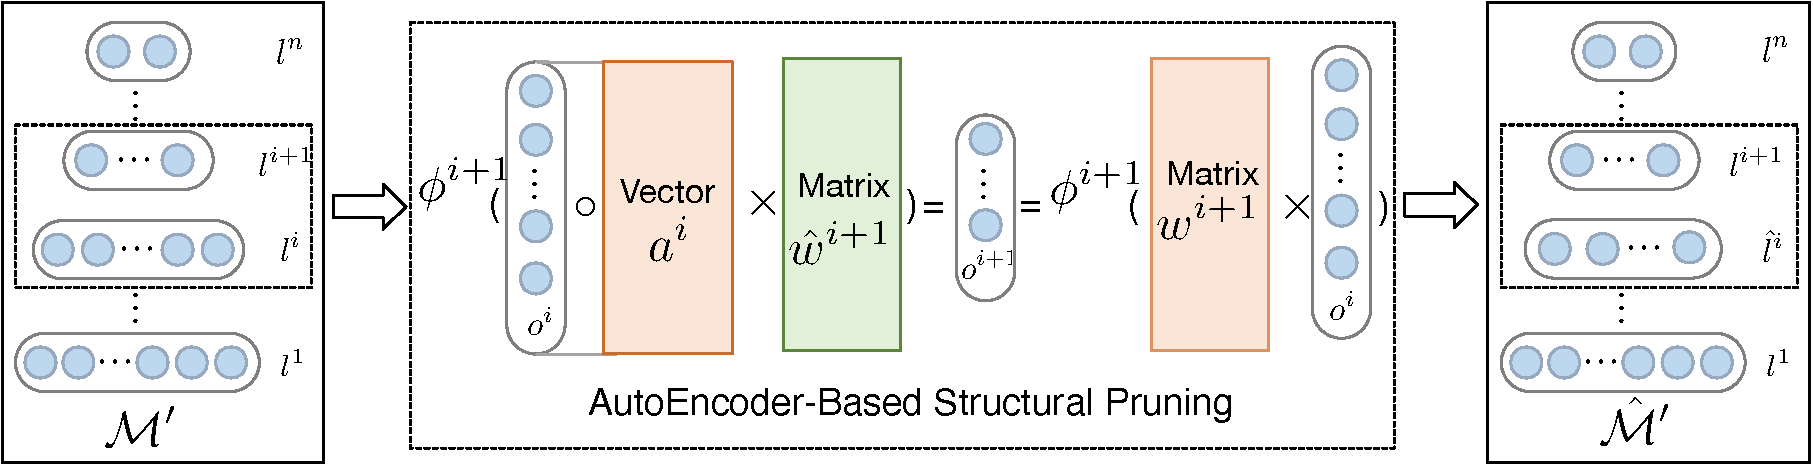
\includegraphics[width=0.9\textwidth]{fig/RP_TASK3_pruning.pdf}
    \caption{Model pruning for robust DNN.}
    \label{fig:task3_pruning}
\end{figure}

 To address the optimization problem in Equation~\eqref{eq:pruning_target}, previous studies~\cite{luo2017thinet, jiang2018efficient} focus on given pruning rates and select the pruning neurons by iteratively updating the binary mask via the greedy selection and weight update. In this project, we propose an auto-encoder-based structural pruning method to learn a binary mask for automatic layer-wise model pruning in Figure~\ref{fig:task3_pruning}. According to Figure~\ref{fig:task3_pruning}, we conduct layer-wise pruning on robust model $\mathcal{M}'$ through the reconstruction of the weight matrix of two adjacent layers. Specifically, motivated by Equation~\eqref{eq:l_pruning}, we use a encoder network to model the mask process and a decoder network to recover the input $o_i$ for layer $l^i$. Here, we iteratively train the binary mask for each layer in model $\mathcal{M}'$ from bottom to top. 
 
 Compared with previous methods, our proposed one enables two advantages: (1) Our method selects the pruning neurons automatically without a specified pruning rate; (2) The by-product of the structure $\hat{w}^{i+1}$ for layer $l^i$ is performance-preserving and no extra fine-tuning process is required. Here, considering the input $a^i$ of this auto-encoder is data-related ($a^0$ in the first layer is actually the input data), the parameters in this autoencoder can be updated by the training set. Regrading the optimization-enabled update process, the objective function is composed of the following parts:
\begin{itemize}
    \item Reconstruction loss. Reconstruction loss aims to guarantee the minimum distance of the outputs of the encoder and decoder. The Reconstruction loss can be presented as:
    \begin{equation}\label{eq:reconstruction_loss}
        \mathcal{L}_{RC} =  
     \frac{\alpha}{2m_{i+1}}\|\phi^{i+1}(o^i\times w^{i+1}+b^{i+1}) - \phi^{i+1}(o^i\circ a^i\times \hat{w}^{i+1}+\hat{b}^{i+1})\|^2_2,
    \end{equation}
    where $\alpha$ denotes the scaling factor.
    \item Maximum pruning loss. Maximum pruning loss aims to remove the weights in a layer to the utmost extent. considering the pruning mask is a binary vector, the maximum pruning loss can be presented as:
    \begin{equation}
        \mathcal{L}_{MP} = \beta \sum_{j=1}^{m_{i+1}} a^{i,j},
    \end{equation}
    where $\beta$ denotes the balancing coefficient.
    \item Performance-preserving loss. To maintain the robustness of the robust $\mathcal{M}'$, the trained encode vector is expected to be close with the initial encoder vector $o^{i+1}$, the loss can be presented as:
    \begin{equation}
        \mathcal{L}_{PP} =  \frac{\gamma}{2m_{i+1}}\|o^{i+1} - \phi^{i+1}(o^i\circ a^i\times \hat{w}^{i+1}+\hat{b}^{i+1})\|^2_2,
    \end{equation}
    where $\gamma$ denotes the scaling factor.
\end{itemize}

Finally, the loss for the optimization $\mathcal{L}_{pruning}$ is:
\begin{equation}
    \mathcal{L}_{pruning} = \mathcal{L}_{RC}+\mathcal{L}_{MP}+\mathcal{L}_{PP}.
\end{equation}

Noted that original binary network is hard to converge, here soft mask technique is utilized ($a^i=\{a^{i,j}|a^{i,j}\in \mathcal{R}^{m_i}_{j=1}, 0\le a^{i,j}\le 1$). In addition, two-step optimization from FISTA~\cite{denton2014exploiting} is introduced to solve the optimization of $a^i$ and $\hat{w}^i$.

After the iteration of the structural pruning, we can obtain a pruned model $\mathcal{M}^{''}$, where the new structure in layer $l^i$ and the corresponding weights $\hat{w}^{'}$ are from the trained auto-encoder. In this project, we will further explore the formal verification techniques in \textbf{Task 4} to verify the preserved robustness of the pruned model $\mathcal{M}^{''}$ and certificate it with a quantified score.
\subsection{Task 4: Quantitative robustness verification of DNN models.}
\textcolor{blue}{From \textbf{Task 3}, we get the neural network model $\mathrm{M}''$ after reduction and optimization. The dataset $\mathcal{D}$ is from \textbf{Task 2}. The neural network is presented as $\langle L,W,B,\Phi \rangle$. $L=\lbrace l^{0},\dotsm,l^{n} \rbrace$ is the set of layers of $\mathrm{M}''$ where $n\in \mathbb{N}$. $l^{0}$ and $l^{n}$ are the input layer and output layer. 
For $k\in\lbrace1, \dotsm,n-1\rbrace, k\in\mathbb{N}, \forall{l_{k}}$ is the hidden layers of $\mathrm{M}''$ with $v_k\in\mathbb{N}^{k}$ dimensions. 
$W=\lbrace w^{1}, \dotsm, w^{n}\rbrace$is the set of weight matrices for layer 1 to \emph{n}. For $\forall k\in\lbrace 1,\dotsm,n\rbrace$, $w^{k} \in \mathbb{R}^{v_k \times v_{k-1}}$ is the weight matrices from $l^{k-1}$ to $l^k$. $w^k_{i,j}$ is the value of \emph{i}-th row and \emph{j}-th column value of $w^k$ where $i,j \in \mathbb{N}$ and $i\in v_k, j\in v_{k-1}$.
$B=\lbrace b^{1}, \dotsm, b^{n} \rbrace$ is the set of bias vectors for each layer, and for $\forall k\in\lbrace 1,\dotsm,n\rbrace$, $b^{k} \in \mathbb{R}^{v_k}$. $b_i^{k}$ is the bias value of \emph{i}-th neuron in \emph{k}-th layer.
$\Phi=\lbrace \phi^{1}, \dotsm, \phi^{n}\rbrace$ is the set of activation functions, such as ReLU, Sigmoid and Softmax, for layer 1 to \emph{n} or $n-1$. 
$z^k_i$ is the neuron value after activation function of \emph{i}-th neuron of \emph{k}-th layer.
}

\begin{equation}
    z^{k}_i=\phi^{k}(w^kz^{k-1}+b^k) = \phi^{k}(\sum_{n-1}w^{k}_{n,i}z^{k-1}_i + b^{k}_{i}), 1 \leq k \leq n.
\end{equation}

The neural networks from \textbf{Task 3} are various based on the requirements of industries and businesses. Due to the differences in neural network structures and analysis components, the verification approaches need to be designed. From the neural networks structure view, there are convolutional neural networks for computation vision and speech recognition, recurrent neural networks for text processing and image tagging, and modular neural networks for video processing. From the analysis components view, the verification works on activation functions, weight, and bias. In \textbf{Task 4}, we will propose several methods to cover the quantitative robustness verification of different kinds of neural networks.

The quantitative robustness verification procedure starts by analyzing the neural network input space and determining the space feature. We will determine the place to insert the perturbation. After these, the fusion of input space and perturbation will generate the unique abstract robustness verification constraints. Optimizing spaces and constraints (such as approximating a finite set of space for required accuracy) improve computational efficiency. Finally, there will be multiple ratios to represent the quantitative robustness.

\begin{table}[!ht]
\centering
    \begin{threeparttable}    
    \caption{}
        \begin{tabular}{p{1.9cm}| p{3.8cm}| p{2.5cm}| p{3.8cm} |p{2.3cm}}
            \toprule
            \textbf{Category} & \textbf{Objective} & \textbf{Method} & \textbf{Approach} & \textbf{Input/Output\tnote{1}}\\ 
            \hline\hline
            \multirow{3}{*}[-0.5\dimexpr \aboverulesep + \belowrulesep + \cmidrulewidth]{Reachability} & \multirow{3}{*}[-0.5\dimexpr \aboverulesep + \belowrulesep + \cmidrulewidth]{\shortstack{Layer-by-layer to \\ compute reachable \\ set $\mathcal{R}\lbrace \mathcal{X},\mathbb{N}\rbrace$} }
                & ExactReach\cite{xiang2017exactreach} & Exact Reachability & HP/HP(bound) \\ \cline{3-5}
            & & AI2\cite{gehr2018ai2} & Split and Join &HP/HP(bound)\\ \cline{3-5}
            & & MaxSens\cite{xiang2018maxsens} & Interval Arithmetic &HP/HP(bound)\\ 
        \hline
            \multirow{3}{*}[-0.5\dimexpr \aboverulesep + \belowrulesep + \cmidrulewidth]{\shortstack{Primal \\ Optimization}} & \multirow{3}{*}[-0.5\dimexpr \aboverulesep + \belowrulesep + \cmidrulewidth]{\shortstack{$\min \limits_{x,y} o(x,y, \mathcal{X}, \mathcal{Y})$, o is \\ the objective function\tnote{2} } }
                & NSVerify \cite{lomuscio2017NSVerify} & Naive MILP & HR/PC         \\\cline{3-5} 
            & & MIPVerify \cite{tjeng2017MIPVerify} & MILP with bounds & HR/PC  \\\cline{3-5}
            & & ILP \cite{bastani2016ILP} & Iterative LP & HR/PC            \\
        \hline
            \multirow{3}{*}[-0.5\dimexpr \aboverulesep + \belowrulesep + \cmidrulewidth]{\shortstack{Dual \\ Optimization}} & \multirow{3}{*}[-0.5\dimexpr \aboverulesep + \belowrulesep + \cmidrulewidth]{\shortstack{A valid bound of output \\ constraints violation}} 
                & Duality\cite{dvijotham2018duality} &Lagrangian Relaxation  & HR(uni)/HS\\\cline{3-5} 
            & & ConvDual\cite{wong2018ConvDual}& Convex Relaxation& HR(uni)/HS\\\cline{3-5} 
            & &Certify\cite{raghunathan2018certify} & Semidefinite Relaxation&HR(uni)/HS \\
        \hline
            \multirow{3}{*}[-0.5\dimexpr \aboverulesep + \belowrulesep + \cmidrulewidth]{\shortstack{Search and \\Reachability}} & \multirow{3}{*}[-0.5\dimexpr \aboverulesep + \belowrulesep + \cmidrulewidth]{\shortstack{Search in the input or \\ the hidden spaces for\\ a counter-example}} 
                & ReluVal\cite{wang2018ReluVal} &Symbolic Interval & HR/HR\\\cline{3-5} 
            & & Fast-Lip\cite{weng2018fast} & Lipschitz Estimation & HR/HS\\\cline{3-5} 
            & & Fast-Lin\cite{weng2018fast}  & Network Relaxation & HR/HS\\
        \hline
            \multirow{4}{*}[-0.5\dimexpr \aboverulesep + \belowrulesep + \cmidrulewidth]{\shortstack{Search and \\ Optimization}} & \multirow{4}{*}[-0.5\dimexpr \aboverulesep + \belowrulesep + \cmidrulewidth]{\shortstack{Utilize the piecewise \\ linearity of activation \\ function to efficiently \\ compute output bounds }} 
                & Sherlock\cite{dutta2017Sherlock} &Local and Global Search & HR/HR(1-D)\\\cline{3-5} 
            & & BaB\cite{bunel2018BaB}& Branch and Bound & HR/HR(1-D)\\\cline{3-5} 
            & & Planet\cite{ehlers2017Planet} & Satisfiability (SAT) &HR/PC \\\cline{3-5} 
            & & Reluplex\cite{katz2017reluplex} & Simplex &HR/PC \\  
        \bottomrule
        \end{tabular}
    
    \begin{tablenotes}
        \item[1] HR: Hyper Rectangles; HS: Half Spaces; HP: Half space Polytopes; VP: Vertex Polytopes; PC: Polytope Complements \\
        \item[2] Objective functions: minimax disturbance, minimal summation, and maximal summation.
    \end{tablenotes}
    \label{tab:verification_method_summary}
\end{threeparttable}
\end{table}

\begin{comment}
    The quantitative robustness of the DNN model measures the uncertainty of the model and certifies whether the estimated effects of the interest are sensitive to the guided specifications. In the literature, the robustness of a model has been defined in different ways: (1) as a weighted average effect to the output~\cite{severyn2015twitter, goodfellow2015explaining}; (2) effect stability in cases~\cite{zheng2016improving}; (3) the minimum adversarial frequency radius to encounter a misclassification corner case.
\end{comment}


The robustness of $\mathcal{N}$ is checking by $Robust(\mathcal{N},x,\mathtt{p},d)$, ($x\in \mathbb{R}^n \subseteq \mathcal{X}$, $x$ is the input and $\mathcal{X}$ is domain of $x$.) to certify $\mathcal{N}$ returning the same outputs when supplying all inputs in the $d$- distance of $x$ under $\mathtt{p}$ normalization. $Robust(\mathcal{N},x,\mathtt{p},d)$ is reasoning the input and output constraints below to \texttt{True} or \texttt{False}, which indicates the given $\mathcal{N}$ is whether robust or not, respectively.
\begin{equation}
    \mathcal{X} = \{ x' |\ ||x-x'||_{\mathtt{p}} \leq d \}
\end{equation}
\begin{equation}
    \mathcal{N(X)} \subseteq \{ y'|\ class(y) = class(y') \}
\end{equation}

If $Robust(\mathcal{N},x,\mathtt{p},d)$ holds \texttt{True}, we certify $\mathcal{N}$ is robust $w.r.t$ $x$ within $d$- distance under the $\mathtt{p}$ norm sharing same the prediction class as $y$, where $\mathtt{p}$ can be 1, 2, or $+\infty$. The network neuron in the output layer is the final $y$ to be recursively obtained by: 


\begin{figure}[t]
    \centering
    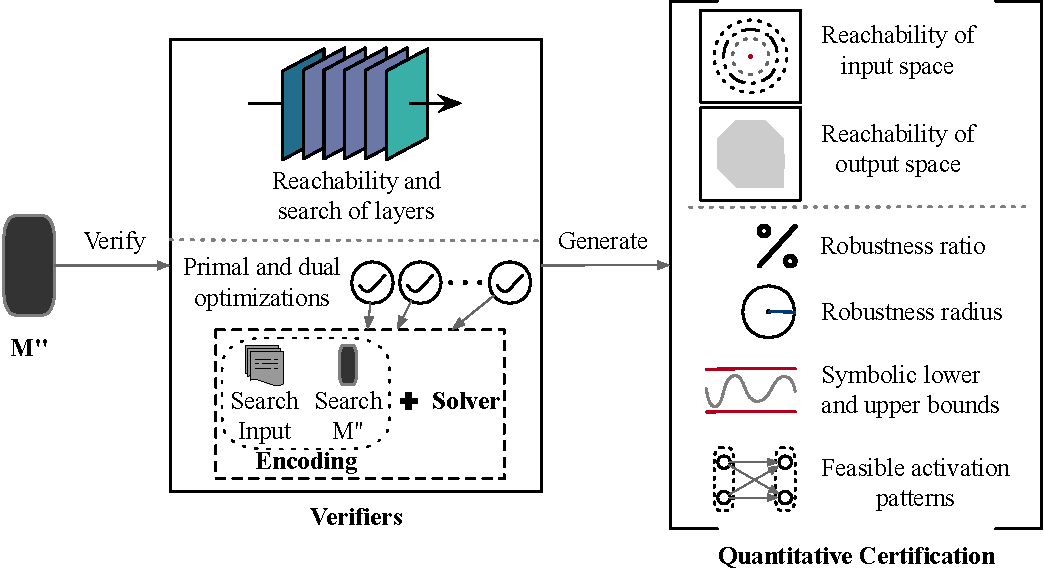
\includegraphics[scale=0.75]{fig/task4.pdf}
    \caption{Quantitative verification}
    \label{fig:task4}
\end{figure}

\textcolor{pink}{indicators of quantitative certification}

\textcolor{blue}{We will propose multiple quantitative verification approaches for generating a certification. The first category of approaches is the reachability of the input and output space through searching the network layers. More specifically, given an input constraint, the approaches will propagate the geometric sets layer by layer from the input layer to the output layer to get the reachable set. There is a comparison between the reachable set and the existing output constraint. The reachability will hold if contained; otherwise, the property is not held. The second category of approaches is the primal and dual optimizations through encoding and solving the input space and model. More specifically, the model will be encoded to model counting constraints and verified through abstract symbolic execution and model generation at symbolic execution tree nodes. The quantitative robustness certification consists of the reachability of input and output space, robustness ratio, robustness radius, lower and upper bounds, and feasible activation patterns. The quantitative verification processes are in Figure~\ref{fig:task4}.}

\textcolor{blue}{\textbf{Input and output space reachability}.  The reachability of input space and output space are denoted as $\mathcal{R}_{input}(\mathcal{X})$ and $\mathcal{R}_{output}(\mathcal{Y}, \mathrm{M}'')$. $\mathcal{X}$ is the input dataset with \emph{m} records and \emph{n} dimensions. $d_{i,j}$ is the value in $\mathcal{X}$. $\mathcal{Y}$ is the expected output set of $\mathcal{X}$ at the same row. }
\begin{equation}
\mathcal{R}_{input}(\mathcal{X})=\left[ (\min_{\genfrac{}{}{0pt}{2}{i=0,\dotsm,n-1} {0}} d_{i, 0},\max_{\genfrac {}{}{0pt}{2}{i=0,\dotsm, n-1 }{0}} d_{i, 0}),\dotsm, (\min_{\genfrac{}{}{0pt}{2}{i=0,\dotsm, n-1}{j-1}}d_{i, j-1},\max_{\genfrac {}{}{0pt}{2}{i=0,\dotsm, n-1}{j-1}} d_{i, j-1}) \right] s.t. \mathcal{R}_{output}(\mathcal{D}_{in}, \mathcal{N}) \subset \mathcal{D}_{out}
\end{equation}


\textcolor{blue}{\textbf{Robustness ratio}. For a neural network $\mathcal{N}$, an input $\mathcal{X}=\langle x_0, \dotsm, x_{n-1} \rangle$, a perturbation limit $\mathcal{P}^{lim}= \langle p^{lim}_{0}, \dotsm, p^{lim}_{n-1} \rangle$ denoting the perturbation limit value per feature, $S_{Area}$ denoting all perturbed inputs within $\mathcal{P}^{lim}$, $S_{RobustArea}$ denoting all perturbed inputs within the limit that the output of $\mathcal{N}$ does not change, $\bar{X}$ denoting the set of $x_i\in \mathcal{X}$ within the conditions.  The robustness ratio $R_{r}$ calculates as follows.}

\begin{equation}   R_{r}(\mathcal{N},\mathcal{X},\mathcal{P}^{lim})=\frac{\lvert S_{RobustArea}\rvert}{\lvert S_{Area}\rvert}
\end{equation}
\begin{equation}
    S_{RobustArea}=\lbrace\bar{X}|\:arg\:max\:\mathcal{N}(\bar{X}) =arg\:max\:\mathcal{N}(\mathcal{X})\:\:\wedge\:\: x_i-p^{lim}_i\leqslant \bar{x_i}\leqslant x_i + p^{lim}_i\rbrace
\end{equation}
\begin{equation}
    S_{Area}=\lbrace\bar{X}|\:\: x_i-p^{lim}_i\leqslant \bar{x_i}\leqslant x_i + p^{lim}_i\rbrace
\end{equation}

\textcolor{blue}{\textbf{Robustness radius.} Given a network $\mathcal{N}$, an input \emph{x}, a norm $\mathtt{p}$, and a distance $d$, the maximum robustness radius ($MRR$) is to compute the minimum distance from input \emph{x} to a counterexample \emph{x'}.}
\begin{equation}
        MRR(\mathcal{N},x,\mathtt{p},d)=\max_{d}\left\{ \left\| x-x' \right\|_\mathbf{p} < d \ |\  Robust({\mathcal{N}, x',\mathtt{p},d}) == \texttt{True},\  \mathcal{N}(x) = \mathcal{N}(x')\right\}
\end{equation}

\textcolor{blue}{\textbf{Lower and upper bounds.} The lower and upper bounds on $v_{i,j}$ which is the value of node \emph{j} on layer \emph{i} before activation function $\sigma$ are denoted as $l_{i,j}$ and $u_{i,j}$. $l_i$ and $u_i$ denote the lower and upper bounds of \emph{i}th layer $v_i$. The lower and upper bounds on $\hat{v}_{i,j}$ which is the value of node \emph{j} on layer \emph{i} after activation function are denoted as $\hat{l}_{i,j}$ and $\hat{u}_{i,j}$. The lower and upper bounds of \emph{i} layer before activation function are $L_i=\max l_{i,j}$ and $U_i=\max u_{i,j}$. $\hat{L}_i=\min \hat{l}_{i,j}$ and $\hat{U}_i=\max\hat{u}_{i,j}$ are the lower and upper bounds of \emph{i} layer after the activation function. }
\begin{equation}
    l_{i,j}= \min_{v_{i-1}\in [ l_{i-1}, u_{i-1} ]  } w_{i,j} v_{i-1} +b_{i,j}
\end{equation}
\begin{equation}
    u_{i,j}= \max_{v_{i-1}\in \left [ l_{i-1}, u_{i-1} \right ]  } w_{i,j} v_{i-1} +b_{i,j}
\end{equation}
\begin{equation}
    \hat{l}_{i,j}= \min_{v_{i,j}\in \left [ l_{i,j}, u_{i,j} \right ]  } \sigma_{i,j} (v_{i,j})=\sigma_{i,j}(l_{i,j})
\end{equation}
\begin{equation}
    \hat{u}_{i,j}= \max_{v_{i,j}\in \left [ l_{i,j}, u_{i,j} \right ]  } \sigma_{i,j} (v_{i,j})=\sigma_{i,j}(u_{i,j})
\end{equation}

\textcolor{blue}{\textbf{Feasible activation patterns}.}

\textcolor{pink}{new: handling more activation functions}

\textcolor{blue}{ Current verification approaches handling piece-wise linear activation functions mainly consider ReLU functions. A few consider Sigmoid and Softmax. The verification approaches in our project will handle other activation functions such as Exponential Linear Units (ELUs)~\cite{clevert2015fast} speeding up comparing ReLU on ImageNet and Gaussian Error Linear Unit(GELU)~\cite{hendrycks2016gaussian} outperforming in CV and NLP tasks. }

\textcolor{pink}{new: handling RNN}

\textcolor{blue}{The input of task 4 will have feedforward neural networks and recurrent neural networks (RNN). Current research works on feedforward neural networks. We will propose a method to transform RNNs into feedforward neural networks to adapt to verification approaches.}




\begin{comment}
\begin{figure}[t]
    \centering
    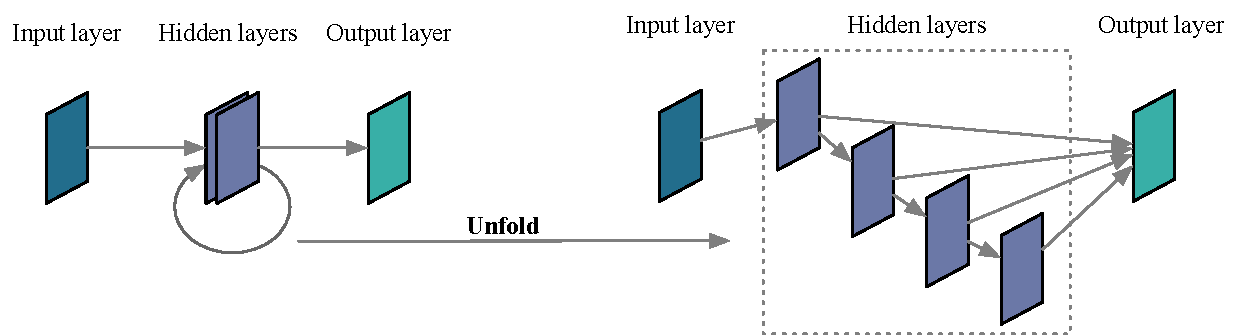
\includegraphics[scale=0.65]{fig/unfoldRNN.pdf}
    \caption{Unfold RNN to feedforward neural network}
    \label{fig:unfold}
\end{figure}
\textcolor{green}{balance between accuracy and scalability}

To calculate the decision boundary (between malicious and benign), we need only apply what ever learner we are uses to its own training data. This will assign classifications (malicious or benign) to every training example. Then, for each example:
\bi
\item Find its nearest neighbor with a different classification;
\item Sort every example by its distance to its nearest unlike neighbor;
\item Look a the top (say) 100 pairs.
\ei
Then, to see it two learners have the same boundary, compute the Jaccard index (intersection divided by overlap) of their top 100 pairs.
  



    \subsubsection{Trade-offs and Risks}\label{r1}
This part is the foundation of the following learning strategies. 
However, the following research will be delayed if too much time is spent on this task. 
Hence, we will conduct some simple studies to sort these factors and continue the studies following this ranking. 
Then, if this task takes too long, we might analyze the current results and move to \textbf{GOAL2} on these results.
\end{comment}



% \section{Schedule} 


 \begin{wraptable}{r}{3.35in}
{ \footnotesize
\begin{tabular}{|l|l|l|l|}\cline{2-4}    
\multicolumn{1}{c|}{~}      &\multicolumn{3}{c|}{Year} \\
\multicolumn{1}{l|}{~}       &1 & 2 & 3  \\\hline  
{\bf Goal2:} run faster                   &   x  &  &   \\\hline 
{\bf Goal1:} better post-attack performance         &    x  &       &   \\\hline 
{\bf Goal3:} test against adaptive adversaries        &      & x      &   \\\hline  
{\bf Goal4:}  test in numerous domains                &      & x     &       \\ \hline
{\bf Goal5:} inspect the decision boundaries           &      & x      &  x     \\ \hline
BPC work (broadening participation in computing)  &   x &  x    & x     \\ \hline
\end{tabular} } 
\caption{Timetable for this work. }\label{when}
\end{wraptable}
Table~\ref{when} shows a three-year plan from this work.
Note that   will explore {\bf GOAL2} first since, if successful, this will speed up everything else.
Also,  we   explore {\bf GOAL5} last since everything up till
then has the potential to change the generated decision boundaries.

Lastly, 
one  of the benefits of  NSF funding
is the opportunity to work on  broadening participating in computing (BPC).  Our BPC plans are discussed in \S\ref{bpc}. As seen
  in our timetable, BPC will be an on-going task through-out the work.

% \subsection{Other Details}
% This NSF solicitation has certain required
% headings. Much of the information needed for those headings
% has already been presented. That said, we aggregate that information here.

% \subsubsection{Results from prior CSSI awards}

% This proposal is based on prior results generated from
% Elements: Can Empirical SE be Adapted to Computational Science? Award \#1931425
% (PI= Dr. Tim Menzies, NCState. 2019-2022).
% Problems with COVID   meant that we could
% not attend enough CSSI meetings to contact more groups.
% That said, using telecommunication tools,
% we spend much time interviewing CSS developers looking for their specific project needs.
% Samples of results from that CSSI were presented in 
% \fig{health} and 
% Table~\ref{casestudy}. 
 

% \subsubsection{Cyberinfrastructure Plans}

% As said in our introduction,  
% a unique feature of this proposal is its scope.
% All the tools generated by this  project  will  be  placed  on-line  in  a  free-to-access  Github  repository  and  made  available  to  the  CSS community via an open source license.
% The software produced here will be applicable to  {\em any} CSS project using an open source repository (and we know at least 700 such projects). In our concept of operation 
% for any project  registered  with {\IT},
% whenever developers commit code, they automatically receive an issue report commenting on the current and future health of their software, along with advice on how to improve that future state.  
 
%  \subsubsection{Measurable Outcomes}
% In terms of measuring the success of this work,
% those  
%  \textcolor{red}{{\bf measurable outcomes}} are listed in red (see above).
 
%  Also,  all the code developed as part of this work will be  released as open-source software in GitHub, under an MIT license.  Included in those
% packages will be the data used to certify the scripts as well as {\em RQn.sh} files containing executable scripts to reproduce (e.g.) RQ1.



%   \subsubsection{Management and Coordination Plan}
  
%   As said in our introduction, it is not enough to merely advertise some service and expect the community to use it. Much of the funds requested by this work is for  NC State researchers  to 
%   analyze as many CSS projects as possible. With these preliminary results in hand, they will approach CSS projects offering commentaries on their software (derived via our data miners)  and free consulting services on how to improve those projects. By  enticing CSS project members with results from their own projects, we anticipate growing a large user base amongst the CSS community.
  
 

 

%  \subsection{Related work in the Explanation Literature}
 

% When discussing this work with colleagues, they sometimes comment that
% xPLAIN is more a ``planner'' (on what to change) than an   ``explaination''
% device.
%  To those colleagues,
%   we  reply that there
%  is
% much precedent in the AI literature
% for connecting planning to explaination.
% In their systematic literature review on AI and explanation, 
%  Violane et al.~\cite{vilone2020explainable} use terminology that we find to be synonymous with our
%   plans that recommend what to change in order to most improve a system.  Violane et al. report is that
%   one of the 
%  most widespread use of explanations
%  in AI is to  find ways to change a
%  models behaviour; e.g. to debug a system in order
%  to stop some bug reoccurring).  
 
%  Other researchers make analogous conclusions.
% Adadi and  Berrada~\cite{Adadi18} list
% four main motivations for building
% explanation systems: 
% (a)~{\em explaining to justify} decisions made
% by some  model;
% (b)~{\em explaining to control} a system,
% allowing its debugging and the identification of potential flaws;
% (c)~{\em  explain to improve} 
% predictive performance and/or efficiency;
% and 
% (d)~{\em explaining to discover} novel  relationships and patterns in the data. As shown by the examples
% below, our ``planning as explanation'' methods  address motivation (b,c,d).

% Furthermore, the Violane et al. review
% lists no less than 37
% terms connected
% to current AI papers discussing  ``explaination''\footnote{
% Algorithmic transparency, 
% actionability, 
% causality, 
% completeness, 
% comprehensibility, 
% cognitive, 
% correctability, 
% effectiveness, 
% efficiency, 
% explicability, 
% explicitness, 
% faithfulness, 
% intelligibility, 
% interactivity, 
% interestingness, 
% interpretability, 
% informativeness, 
% justifiability, 
% mental fit, 
% monotonicity, 
% persuasiveness, 
% predictability, 
% reversibility, 
% robustness, 
% satisfaction, 
% scrutability / diagnosis, 
% security, 
% selection/simplicity, 
% sensitivity, 
% simplification, 
% soundness, 
% stability, 
% transparency, 
% transferability and, 
% understandability}.
% Semi-supervised planning relates to at 
% least two of the terms in the  
% Violane et al. survey: actionability and  effectiveness (since both these terms comment on if a plan can be deployed and (after that) how well the plan actually works.

  
  
 \section{Intellectual Merit and Broader Impact}
 \subsection{Intellectual Merit}
 The     OMNI-1  results suggests that  prior work made a premature and 
 incorrect conclusion about the value of diversity-based defences (against adversarial learning).  
   The use of ensembles
 has its
defenders~\cite{kariyappa2019improving,biggio2010multiple,DBLP:conf/iclr/TramerKPGBM18,smutz2016tree,kantchelian2016evasion} and it detractors~\cite{zhang2020decision,zhang2018gradient,he2017adversarial,DBLP:conf/iclr/TramerKPGBM18,DBLP:journals/corr/PapernotMG16}. 
Here, 
 we argue here before we can use ensembles to defend against attackers, we need to change the way we build and use ensembles.  Specifically, our ensembles based their  conclusions come from exploring the 
 {\em far corners of a very large ensemble}, rather than just the center
of a   small ensemble. 


  Prior work   concluded
    that    different  defending
  learners generate the  same decision boundary
  (the region separating malicious from benign inputs). This is highly
  undesirable since it  mean
   attackers can also learn that structure, {\em even if the attacker does not know
  the learner being used by the defender}.  Yet if this were always so, then OMNI-1 
  would not have worked.  The possibility, to be explored here with OMNI-1, is that  if we jump around a very large range of defense options, we can effectively defend against a wide range of adversarial attacks. 
  
  

 


\subsection{Broader Impacts} 

The more the international community connects (via software), the more that community
is susceptible to attacks. 
 This work will increase America’s ability for industrial and academic innovators to secure their own
 work.  
This in an important area of research since there  is an increasing reliance of
computational methods in all aspects of our society. 

 
 
As to other broader impacts, NC State's Computer Science department has a strong record of studying research issues related to gender bias~\cite{pullreq_17}, barriers faced by women ~\cite{ford2016paradise}, and methods for broadening participation~\cite{selfies} in the context of software engineering. 
 This work will inform the curriculum  and lecture notes of the various NC State NSF-funded REUs (research experience for undergraduates) as well as graduate
SE classes (taught by PI Menzies).  
PI Menzies will continue his established tradition of graduating research students for historically under-represented groups.
Also, funds from this work will be used to support students attending the Grace Hopper conference,
and the Richard Tapia Celebration  of Diversity in Computing.



Finally,  a (small) portion of this grant would be allocated to support Broadening Participation in Computing (BPC) work
(see next section).

 
 
 

\subsection{BPC Work: Broader Participation in Computer Science} \label{bpc}



  PI Menzies is a member of
his department's Broadening Participation Committee (BPC) that actively seeks to:
(a)~{\em Understand} what factors make computer science
more (or less) attractive to underrepresented groups;
(b)~{\em Educate} faculty, staff, and students on how different behaviors   effect diversity, quality and inclusiveness;
(c)~{\em Increases} the percent of students who identify as women; 
and (d)~{\em Evaluate} the success of his department's BPC team in broadening
participating.
 

 
\subsection{Dissemination of Knowledge}

All the code developed as part of this work will be  released as open-source software in GitHub, under an MIT license.  Included in those
packages will be the data used to certify the scripts as well as {\em RQn.sh} files containing executable scripts to reproduce (e.g.) RQ1.

  As to papers, PI Menzies frequently publishes as top-ranked international scientific venues and it is  anticipated that this work will generated multiple papers at
such venues. 

Also, this work will generated much  material (tools, scripts, data sets) that can be utilized by other research teams. 
For  a decade, PI Menzies has  lead-by-example in the open science community (the PROMISE project and the ROSE initiative) which takes care
not only to package and distribute research code but also publish papers and tutorials on that material.  
 


%  \section{Prior Results}\label{sec:PriorResults}

PI Menzies is an IEEE Fellow and has earned over \$13 million dollars in peer-reviewed competitive grants (\$6.4M from NSF, and  the rest for a variety of other government and industrial sources).
Google Scholar lists him as a top-ten researcher in many research areas including knowledge acquisition and analytics. Serving as committee chair, he has graduated 12 Ph.D. and 32 masters students (by research). He currently supervises 10 Ph.D. students at NC State. He has served as an associated editor on all the major SE journals and from 2021 will be EIC of the Automated Software Engineering journal. 


 We include below some notes  on some of his most recent NSF grants.

% PI Menzies is a co-PI with    Dr. Laurie Williams  working  on \underline{(a)}~CCF-1909516, 2019-2022, \$499,998; \underline{(b)}~``SHF: Small: Detecting the 1\%: Growing the Science of Vulnerability Detection''; \underline{(c)}~The {\bf intellectual merit} of that work was to explore characteristics of vulnerabilities with a focus on those that pose the highest security risk. The {\bf broader impact} of that work was to improve the ability of practitioners to produce secure software products so that people can rely upon computer systems to perform critical functions and to process, store, and communicate sensitive information securely. \underline{(d)}~That work has generated   journal articles (one at TSE), ICSE publications and one paper under review (at EMSE) \cite{yu2019improving,shu2019improved,elder2021structuring,shu2020omni}. \underline{(e)}~Data from that work is housed at the SEACRAFT publicly accessible repository~\cite{seacraft}. That work funded two Ph.D.s at NCSU. \underline{(f)} N/A.

PI Menzies worked on \underline{(a)}~CCF-1302216, 2013-2107, \$271,553; \underline{(b)}~``SHF: Medium: Collaborative: Transfer Learning in Software Engineering''; \underline{(c)}~The {\bf intellectual merit} of that work was to
define novel methods for sharing data, many of which were the precursor to the methods of this proposal.  That work generated the publications  \underline{(d)}~\cite{krishna2018bellwethers,peters2015lace2,he13,Me17,fu2016tuning,krishna2017learning,krishna2020whence} concerning prediction and planning methods.
The {\bf broader impact} of that work was to
enable a new kind of open science-- one where all data is routinely shared and is capable of building effective models no matter if it is obfuscated for security purposes.
The methods of this project, while targeted at software engineering, could also be applied to any other data-intensive field. \underline{(e)}~Data from that work is now housed in the two
publicly accessible repository\footnote{
{\bf github.com/rshu/Adversarial-Evasion-Defense}}. That work  funded two Ph.D.s at NCSU. \underline{(f)}
N/A. 


% One related data mining grant is \underline{(a)}~OAC-1931425, 2019-2022, \$592,129; \underline{(b)}~``Elements: Can Empirical SE be Adapted to Computational Science?''; \underline{(c)}~The {\bf intellectual merit} of that work was to create a workbench containing methods adapted from empirical software engineering, that would help bridge the skill gap via automatic agents by suggesting to developers when they should investigate or redo part of their code. The {\bf broader impact} is to reduce the associated cost (time, money, etc.) required to handle many of the large and more tedious aspects of software development. \underline{(d)}~That work generated one journal paper (at TSE), an MSR conference
% paper and two other papers under conference review~\cite{agrawal2018better,tu2021mining,tu2020changing}. \underline{(e)}~Data from that work is housed at the SEACRAFT publicly accessible repository~\cite{menzies2017seacraft}. That work funded one Ph.D. at NCSU. \underline{(f)} N/A.

Another relevant research grant is 
\underline{(a)}~OAC-1826574, 2018-2018, 
\$124,628.00;
\underline{(b)}~
``EAGER: Empirical Software Engineering for Computational Science'';
\underline{(c)}~ 
The {\bf intellectual merit} of that work was to
conduct initial explorations into novel methods for adapting SE methods to computational science.
That work lead to the curious
result that, in many ways,
the computational scientists are better
at managing their development cycle
than many SE projects~\cite{tu2020changing}. Whenever
we found good enough data to compare the results
seen in open source and computational
science projects, we often find higher productivity
values (and faster debugging) in computational science
than in software engineering. 
\underline{(d)}~That work generated 
one journal paper (at TSE'21),
one conference paper (at MSR'21) and another journal publication under review~\cite{Ling21}.
 \underline{(e)}~Data from that work is now housed at the SEACRAFT publicly accessible repository~\cite{menzies2017seacraft}. That work  funded one Ph.D. at NCSU. 
 \underline{(f)} N/A.  
 
 
 \newpage

% See also 
% \underline{(a)}~CCF-1703487; 2017-2021,  \$898,349.00; 
% \underline{(b)}~SHF: Medium: Scalable Holistic Autotuning for Software Analytics; 
% \underline{(c)} The {\bf intellectual merit}
% of that work  was that there exist previously unexplored ``short-cuts'' in the search space of control parameters of data miners. The {\bf broader impact}
% was that better learners could be created
% automatically via ``hyperparameter optimizers''
% that exploited those short-cuts. This in term meant
% that anywhere these learners were deployed, they could
% be deployed again with {\em greater} effect. 
% \underline{(d)}~This work generated five journal
% articles at TSE, EMSE, IEEE Software,  
% and one other article currently under review at EMSE~\cite{yedida2021simple,agrawal2020simpler,Yedida21,DBLP:journals/ese/YangCYYM21,menzies2021shockingly,xia2019sequential};  \underline{(e)}~Data from that work is now housed at the SEACRAFT publicly accessible repository~\cite{menzies2017seacraft}. That work  funded two Ph.D. at NCSU.  \underline{(f)}~N/A.
 

  


\end{nsfdescription}

\begin{nsfreferences}
\section*{References}
%kenrefs,proposal,ssl,suvodeep,verifyDNN,HPO,verifyApprs,
      \bibliography{proposal}
\end{nsfreferences} 

\begin{nsffacilities}
  

% \section*{Facilities From other Institutions}
% As stated in our {\em Collaboration Plan},
% we have unpaid collaborators from Facebook,  Microsoft,
% and IBM. Once this research develops viable
% unfairness measurement and mitigation methods
% for semi-supervised algorithms, these collaborators
% will grant us access to materials, to be negotiated, at their
% site. Apart from (potentially) being able to access
% models  behind the firewalls of model stores, an important
% facility these collaborators could offer is access to the subject matter
% experts that can test if the veracity of our
% artificially generated models.


% \section*{Facilities at North Carolina State University}
 
\subsection*{Offices:}
The project PI has
and offices in their   CS Department. This department
has adequate space to house all research assistants
working on this project. All offices are wired for high-speed network access.

The PI's departments at  NC State provide the space and basic networking services to
carry out the experiments, secretarial and administrative support as well as general-purpose office equipment ({\em e.g.}, fax, photocopiers, etc.).

\subsection*{Lab Space}
The PI has their own lab space at NC State.
PI  Menzies' RAISE lab (Real-World 
AI and SE) is a newly renovated space containing over 1,500 ft\textsuperscript{2} of research space and 
15 cubicles, a meeting space, printer, and wide screen projector. 

\subsection*{Compute Facilities}
Part of {\IT} will involve comparatively assessing different technologies. For that process, it will be useful to have some large-scale compute facility.
 
At NCSU, students working on this grant will have access to a 108-node compute cluster named ARC with 2,000 cores (AMD Mangy-Cours), Infiniband QDR interconnect, per node power monitoring, GPUs and SSDs and parallel file system support,
which was funded by an NSF CRI that he is the main PI of together with 5 co-PIs.  
The ARC facility is providing local and remote researchers with administrator/root privileges for Computer Science experiments at a
medium scale. This allows any of the software layers, including the operating system and Infiniband switch network routing tables, to be
modified for experimental purposes, e.g., to experiment with different
network topologies.  For large-scale demonstrations, other 
facilities will be utilized (the HPC discussed below.


Additionally, NC State University provides a High-Performance Computing (HPC) facility as a part of the initiative to provide state-of-the-art support for research and academic computing. HPC system (called henry2) provides NC State students and faculty with entry and medium-level high-performance research and education computing facilities, consulting support and scientific workflow support. The HPC ecosystem consists of 1233 dual Xeon compute nodes in the henry2 cluster. Each node has two Xeon processors (mix of dual-, quad-, six-, eight-, ten-core, twelve-core) and 2 to 6 GigaBytes of memory per core. The total number of cores increases as more cores are purchased and now exceeds 10000. The nodes all have 64-bit processors. All HPC projects have the capability to run jobs using up to 128 processor cores for up to 48 hours and smaller jobs up to a week.
 
%  \section*{Unpaid Collaborators}
 
%  This document contains letter s of 
%  collaboration from:
  
% \be
% \item Tim Menzies,
% North Carolina State University; PI
% \item
%   Anirban Mandal, RENCI, UNC-Chapel Hill; unpaid collaborator (see attached letter).
  
%   \item
%   Wolfgang  Bangerth, Colorado State University, unpaid collaborator (see attached letter).
% \ee
% These researchers were active in our prior CSSI work and offered much useful feedback on our direction
% (as well as case study material).
% We full anticipate that these collaborations will continue.

\end{nsffacilities}

 
\DataManagementPlan{data}
%XXX human data
\newpage
\pagestyle{empty}
 
\section*{Project Personnel}
 
\be
\item Tim Menzies,
North Carolina State University; PI 
\ee


\end{document}


\subsection{Limits to \mbox{OMNI-1}}
As stated in our introduction,
while OMNI-1 was a promising prototype, these
results have numerous limitations that must be addressed.

That said, as stated in the introduction, 
 the \mbox{OMNI-1} study  has certain limitations. 
 For example,
 Figure~\ref{tbl:contagioAccuracy}
 shows results with the \mbox{OMNI-1} and the
 Contagio PDF data set (and the patterns
 shown here repeat across all the other data
 sets of Table~\ref{data}). 

much a  baseline treatment
 reports how well an untuned deep learner can classify known prior attacks as "benign" or "malicious". 
 

To improve om \mbox{OMNI-1}, \mbox{OMNI-2} will explore the following design options:
\bi
\item
The Gower distance allows to assign a weight $w_{ijk}$ to each individual variable base on the importance of that variable in the distance calculation.   \mbox{OMNI-1} used $w_{ijk}=1$, which is
 something that \mbox{OMNI-2} hopes to improve on.  
 \item \mbox{OMNI-1} built its initial pool of configurations using a standard hyperparameter optimization (Hyperopt/TPE~\cite{bergstra2012random}),
 which we think we can improve upon (see \tion{XXX}).
\ei


% \end{tabular}
% \end{table}



% \begin{table}[!h]
% \centering
% \footnotesize
% \caption{An overview of the statistics of the security datasets studied in our work.}
% \begin{tabular}{l|r|c|c}
% \hline
% \rowcolor[HTML]{ECF4FF} 
% \multicolumn{1}{c|}{\cellcolor[HTML]{ECF4FF}\textbf{Dataset}} & \multicolumn{1}{c|}{\cellcolor[HTML]{ECF4FF}\textbf{Original Size}} & \textbf{Sampling Rate(\%)} & \textbf{Feature Count} \\ \hline
% NSL-KDD & 148,517 & 100 & 123 \\ 
% CSE-CIC-IDS2018 & 16,233,003 & 5 & 70 \\ 
% CIC-IDS-2017 & 2,830,743 & 20 & 70 \\ 
% CICAndMal2017 & 2,618,533 & 20 & 71 \\ 
% Contagio PDF Malware & 22,525 & 100 & 135 \\ \hline
% \end{tabular}
% \label{tbl:dataOverview}
% \end{table}



To assess {\bf Omni}, we use the five security datasets of Table~\ref{tbl:dataOverview}
and Table~\ref{tbl:dataInPhase}.
\textit{NSL-KDD}~\cite{nsl-kdd} dataset is an improved version of KDD'99 dataset~\cite{tavallaee2009detailed}, which recorded network traffic under different types of attacks. 
\textit{CIC-IDS-2017}~\cite{sharafaldin2018toward}   is comprised of both normal traffic and simulated abnormal data caused by intentional attacks on a test network.
\textit{CSE-CIC-IDS2018}~\cite{sharafaldin2018toward} is  an intrusion detection dataset that  includes seven different attack scenarios (Brute-force, Heartbleed, Botnet, DoS, DDoS, Web attacks, and infiltration of the network from inside). 
\textit{CICAndMal2017}~\cite{lashkari2018toward} is an Android malware dataset that collects 426 malicious and 1,700 benign applications collected from 2015 to 2017. These malicious samples are split into four categories (Adware, Ransomware, Scareware, SMS Malware) and 42 families.  
\textit{Contagio PDF Malware}~\cite{contagio-pdf} dataset has  labels
on a set of benign and malicious PDF documents
(i.e. those used as delivery vechiles for
malicious content), including a relatively large number from targeted attacks.
 


\begin{table}[!h]
\centering
\footnotesize
\caption{The characteristics of security datasets during training and testing phase.}
\begin{tabular}{l|r|r|r|r|r|r}
\hline
\rowcolor[HTML]{ECF4FF} 
\multicolumn{1}{c|}{\cellcolor[HTML]{ECF4FF}} & \multicolumn{2}{c|}{\cellcolor[HTML]{ECF4FF}\textbf{Training Phase}} & \multicolumn{2}{c|}{\cellcolor[HTML]{ECF4FF}\textbf{Testing Phase}} & \multicolumn{2}{c}{\cellcolor[HTML]{ECF4FF}\textbf{Total}} \\ \cline{2-7} 
\rowcolor[HTML]{ECF4FF} 
\multicolumn{1}{c|}{\multirow{-2}{*}{\cellcolor[HTML]{ECF4FF}\textbf{Dataset}}} & \multicolumn{1}{c|}{\cellcolor[HTML]{ECF4FF}\textbf{Benign}} & \multicolumn{1}{c|}{\cellcolor[HTML]{ECF4FF}\textbf{Malicious}} & \multicolumn{1}{c|}{\cellcolor[HTML]{ECF4FF}\textbf{Benign}} & \multicolumn{1}{c|}{\cellcolor[HTML]{ECF4FF}\textbf{Malicious}} & \multicolumn{1}{c|}{\cellcolor[HTML]{ECF4FF}\textbf{Benign}} & \multicolumn{1}{c}{\cellcolor[HTML]{ECF4FF}\textbf{Malicious}} \\ \hline
NSL-KDD & 67,343 & 58,530 & 12,833 & 9,711 & 80,176 & 68,341 \\ 
CSE-CIC-IDS2018 & 535,701 & 102,379 & 133,926 & 25,595 & 669,627 & 127,974 \\ 
CIC-IDS-2017 & 363,410 & 89,050 & 90,853 & 22,262 & 454,263 & 111,312 \\ 
CICAndMal2017 & 193,777 & 224,873 & 48,445 & 56,218 & 242,222 & 281,091 \\ 
Contagio PDF Malware & 8,821 & 9,199 & 2,205 & 2,300 & 11,026 & 11,499 \\ \hline
\end{tabular}
\label{tbl:dataInPhase}
\end{table}


\section{Other Notes}
\subsection{Scope}
Just to  clarify some remaining points of this
study, this section discusses some of our scoping
decisions. 

 Firstly, we limit the scope of study that the attackers will try to evade a single model with crafted adversarial examples. Attacking multiple models with adversarial examples~\cite{kwon2018multi} is another interesting research direction which we would like to explore in future work.  

Secondly, there is a growing interest in different types of privacy-related attacks (e.g., model extraction attack~\cite{papernot2017practical}) which make the leakage of model information possible~\cite{rigaki2020survey}. For example, Juuti et al.~\cite{juuti2019prada} consider the problem
where a  business model
is hosted in a secure cloud that allow user clients to query the models via cloud-based prediction APIs. These prediction APIs are suffered from being exploited with model extraction attacks. The target model can be used as an oracle for returning predictions for the samples that attackers submit. Such kind of attempts can further be iteratively executed for attackers to maximize the information extraction about model internals. In other proposals to the NSF, we have offered methods to mitigate model extraction attacks.
 





In our method,
we first run a hyperparamter optimizer XXX in the usual manner to find parameters resulting in the model with the highest accuracy. We call this model the {\em expected model} since  
this is the model we would  expect the attackers to learn. 
Note that, as a side effect of this process, we have a large {\em pool} of models; i.e. all the other models explored by the optimizer before arriving at the best one.


  
For this last point \#4 to be effective, we would need to explore a very large space of
configurations.  Certain other   geometric features of 
Figure~\ref{moo} suggest that this is possible.   A commonly observed feature of multi-objective optimizers is
that:
\begin{quote}
{\em Randomly selected
$x$ space configuration decisions  do not spread out evenly in objective $y$ space.}
\end{quote}
More specifically, the $y$ objectives form a {\em surface} within which the achievable
objectives can be clustered into small regions. For example, the standard ROC-surface (receiver operator characteristics) curve of a data miner bows away from the middle of $y$ space towards (but not ever reaching) the ``utopia point''. 




\begin{figure}[!t]
\caption{Reports of a   learner's performance are only reliable within
some epsilon $\epsilon$.  }\label{reach}
\begin{center}
\begin{tabular}{ m{2.5in} m{3.5in} } 
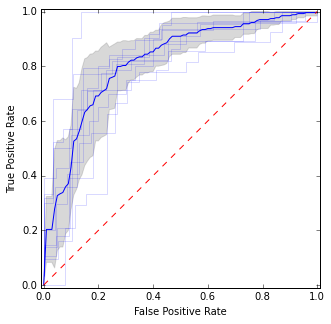
\includegraphics[width=2.5in]{fig/roc.png}&
{\small In this figure thick blue lines shows median performance seen in 10 machine learning
experiments, where each experiment learns on 90\% of the data (selected at random).
Note that  there is some variability seen in the thin blue lines, which are the
results from each individual trial. Comparing the median line to the rest,
we see that there is some variability of size $\epsilon$ in a learner's performance. }
\end{tabular}
\end{center}
\end{figure}

\section{Related Work}


Researchers have proposed various solutions against adversarial machine learning attacks including
  \textit{adversarial training}, \textit{gradient masking}, \textit{defensive distillation}, and \textit{ensemble learning}. The idea of \textit{adversarial training}~\cite{DBLP:conf/iclr/TramerKPGBM18,DBLP:conf/iclr/NaKM18,DBLP:conf/iclr/MadryMSTV18,DBLP:conf/iclr/FarniaZT19,DBLP:conf/nips/ShafahiNG0DSDTG19,yin2019adversarial} is to build a ``golden'' dataset that ideally contains a set of curated attacks and normal data that are representative of the target system. The data is then used when training the model. Intuitively, if the model sees adversarial examples during training, its performance during prediction will be improved for adversarial examples generated in the same way. However, the problem with adversarial training is that it suffers from an optimized attack or adaptive attack, since this method only defends the model against the same attacks used to craft the examples originally included during training. 

\textit{Gradient masking}~\cite{papernot2018sok} is a technique that hides the model gradients to reduce model's sensitivity to adversarial examples. However, later work~\cite{DBLP:conf/icml/AthalyeC018} shows that even with gradient masking,
because of the transferability property of adversarial examples, the attackers can still build a substitute model and transfer the attacks.

\textit{Defensive distillation}~\cite{papernot2016distillation} tries to generate a new model whose gradients are much smaller than the original undefended model. If gradients are very small, some gradient-based attacks are no longer useful, as the attacker would need great distortions of the input data to achieve a sufficient change in the loss function. However, this method can be   ineffective~\cite{DBLP:journals/corr/CarliniW16} since, with a slight modification to a standard attack, attackers can still find adversarial examples on distilled networks.



Thr


Now consider tje
OMNI scores different hypermater configura
While exploring a large number of models (such as the trillions of options from \tbl{hyperparameters}), the ``expected model'' might be the one the scores
best across all the $y$-objectives. ; i.e. the optimal model from hyperparameter optimization, which is used in normal prediction. This model is the target of attackers and hence then becomes the victim model. Next, our optimizer surveys the hyperparameter space of models to find ``unexpected models''; i.e. models that are (a)~performing well (i.e., sub-optimal models) and (b)~dissimilar to the expected model (i.e., in the architecture). More specifically:
\bi
\item 
For hyperparameter optimization, we search a large space of possible configurations of a model to initialize a large \textit{model pool}.
\item
The {\em expected model} is a model from the model pool that performs best (under no attack). We call this model ``\textit{expected}'' since we conjecture that this model would be the target of an attacker, and becomes a victim model.
\item
We introduce an idea called \textit{model distance}, which is a numeric value indicating the degree of similarity of two models' hyperparameter configurations. A large model distance value means that two models are more likely to be different in their model architecture. 
\item The {\em unexpected models} are those whose performance within some small $\epsilon$ of the expected model but are more than some distance $t$ away from the expected model.   
\item
Those unexpected models are combined into a \textit{weighted ensemble}, in which each model $m_i$ in the ensemble with a weight $w_i$. The final prediction of this ensemble is the combined prediction of each model $m_i$ times its weight $w_i$. These weights are further optimized by an evolutionary algorithm that finds optimal $w_i$ setting that maximizes prediction performance.
\item
The final weighted ensemble, with its optimized weight setting is then deployed against evasion attacks.
\ei
  

Software security is often compared to the game ``whack-a-mole'' where players  wait for one or more  furry animals to poke their heads above ground, at which time you
try to ``whack'' them over the head with a large padded hammer before they escape. 

Vulnerability management is often compared to whac-a-mole, with new vulnerabilities appearing up constantly, and security teams realizing that they will eventually fall victim to an adversary. It is common to deprecate such an ad hoc whac-a-mole approach, arguing that security and adversarial defense requires a deep systems approach where the defenders institute long-term policies to (e.g.) deprecate the probability of vulnerabilities being added to a system in the first place.

But what if there was another way to runt the Whac-a-mole game? In our  approach, we turn the tables on adversial attachers 
by (a)~building a very large collection of different defnese algortms, then 
(b)~jumping between them at random at runtime. In this ``reversed Whac-a-mole game'', it is now the attackers
struggling to keep up with all the new tactic of the defenders.

Recent advances in nyperparameter optimziation (HPO) suggest that shis rppach is eindeed viable. As discusses in the next section, such optimziers explore two spaces:
(a)~the space of design decisions for a defnder and (b)~the space of design performance measures. In
standard HPO





of defense


Here, we propose to reverse the rules of that game. Adversarial security
learning is the process of an
external adversary learning examples that confusing internal defending
software
into concluding that some incoming
malicious data is actually benign.
recent results show that even
when the external attack does
not know the internal details,
they can still build a learner
show that an attacker can run a  machine learner ex when
the attackers do not know how
the defender learns to distnushish benign from malcisous inuput, 


A major contributing factor to this problem is that enterprise security teams are overwhelmed with tens of thousands of vulnerabilities across hundreds of thousands of assets that potentially need to be fixed. In an ideal world, you would whack all these moles systematically by “patching all” but this is impossible in most organizations. 




The NSF has spent hundreds of millions of dollars
on computational science software. When those projects fail and are ignored
(or fall into disrepute), then all those monies amount to little more than hard drives
gathering dust in some basement.  How can we find, and fix, faltering computational  science software (CSS)  projects
{\em before} they fail?
To answer this question, this proposal will   develop and certify and apply  the  {\IT} workbench (\underline{\bf M}easuring and mitigating  \underline{\bf U}nhealthy \underline{\bf S}cientific softwar\underline{\bf E}) to CSS software.
{\IT} will be an open source tool with ``hooks'' into source code repository systems such as Github.  {\IT} will distill decades
of work on software analytics into a form easily and rapidly usable by CSS projects. All the tools generated by this project will be placed on-line in a free-to-access Github repository and made available to the CSS community via an open source license.

A unique feature of this proposal is its scope. The software produced here will be applicable to  {\em any} CSS project using an open source repository (and we know at least 700 such projects). In our concept of operation, 
for any project  registered  with {\IT},
whenever developers commit code, they automatically receive an issue report commenting on the current and future health of their software, along with advice on how to improve that future state.  

That said, it is not enough to just advertise a service and expect others to use it. In this work,
NC State researchers will apply {\IT}   to as many CSS projects as possible. With  preliminary results in hand, they will approach CSS projects offering commentaries on their software (derived via our data miners)  and free consulting   on how to improve   projects. By  enticing CSS project members with results from their own projects, we anticipate growing a large user base amongst the CSS community.

\section{Goals}

Parts of {\IT} have been researched an developed for non-CSS software~\cite{peng2021defect,xia2019sequential,xia2020predicting,tu2020changing,tu2021mining}.
But before  we can assert that {\IT}  works on  CSS software, {\IT} needs to be
extend and improved and tested on CSS.
This proposal is a request for funding to perform the research and make the advances
needed to  optimizing  CSS
project corrective recommendations in order to:
\bi
\item {\em Minimize} the data collection required in order to make a recommendation;
\item
 {\em Minimize} the changes associated with {\IT}'s recommendations; 
\item
 {\em Maximize} the effect of {\IT}'s recommendations; 
\item
 {\em Maximize} the likelihood that CSS developers will actually apply those recommendations. 
\ei
% In order to avoid wasted development software effort
% this project will  build predictors for the   success or
% failure of a Computational Science Software (CSS) project. 
% Some CSS projects are more successful that others?
% Why? How early can we see if a project is going to be  more successful that others? If a project is flagging, how soon can we detect that? And
% how can that problem be   repaired? 

\begin{wrapfigure}{r}{3.2in}
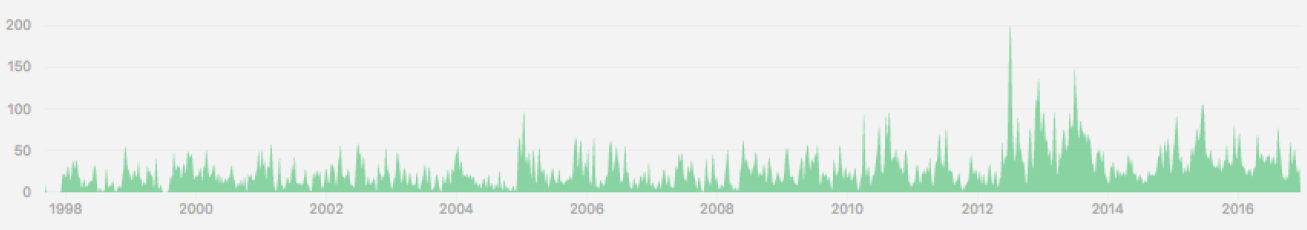
\includegraphics[width=3.2in]{fig/dealii.png}
\caption{Healthy CSS projects are   active. E.g. see the
numerous commits of new software to the deal.II    finite elements 
library since 1998. From  {\bf github.com/dealii}.}\label{fig:dealii}
\end{wrapfigure}
% ~{\IT} is a feasible goal. Our prior CSSI-funded work\footnote{Elements: Can Empirical SE be Adapted to Computational Science?
% Award \#1931425.  PI= Dr. Tim Menzies, NCState. 2019-2022.  }
% has shown regularities in CSS software that,
% in theory, make it amenable to  accurate prediction and repair.  
% When some phenomenon is regular and predictable then it makes it a clear candidate
% for control strategies. Hence this proposal. 
Central to this proposal is the concept of ``project health''.
Researchers agree that ``healthy'' software projects are   ``vigorous'' and ``active''~\cite{han2019characterization, wahyudin2007monitoring,jansen2014measuring,manikas2013reviewing,link2018assessing,wynn2007assessing,crowston2006assessing}. 
For example,   the 
deal.II  adaptive finite elements package  is very 
``healthy''
since,  at the time of this writing,
it  has over 10,000 closed ``pull requests'' (where people
outside the core team have successfully contributed fixes or enhancements).
Another measure of the ``health'' of that deal.ii is that it receives
thousands of commits (changes to its software) each year (see \fig{dealii}).




For non-CSS   software,
PI Menzies and his students 
(Mr. Taianpei Xia~\cite{xia2019sequential,xia2020predicting} and Mr. Huy Tu~\cite{tu2020changing,tu2021mining})
have used early prototypes of {\IT} to successful predicted project ``health''  twenty four months into the future. As discussed below, such information can be used to guide project improvement plans (e.g. improvement planning may be not be required, when a project is predicted to be healthy for the foreseeable future.

That said, those predictions have only be performed on conventional software (i.e. not CSS software). 
As discussed in
\S\ref{prior},
 CSS software  is very different to conventional software. E.g. the latter is subject to the whims of market forces while the former is subject to whims of  funding
agencies. Also, CSS developers are specialists in physics, chemistry, etc and so may lack certain training and experience of SE methods. 
 Accordingly, prior success for predicting health on conventional software needs to be checked for CSS software. Hence our first goal is:
\begin{formal}\noindent
{\bf Goal1}  predict project health for  some CSS projects (discussed in \S\ref{goal1}).
\end{formal}
\noindent
Merely measuring a problem is insufficient. After 
{\em measuring} must come {\em mitigation}. Once
we can  recognize a failing project, the next
step is to seek ways to fix it.
PI Menzies (and his graduate
student Mr. Kewen Peng~\cite{peng2021defect})
have shown that   software can be adjusted to decrease its defects and increase its health. Since  this approach has  yet to tested on CSS software, our next goal must be: 
\begin{formal}\noindent
 {\bf Goal2}  plan effective improvements for some  CSS projects (discussed in \S\ref{goal2}).
\end{formal}





% \begin{wrapfigure}{r}{2.5in}
% 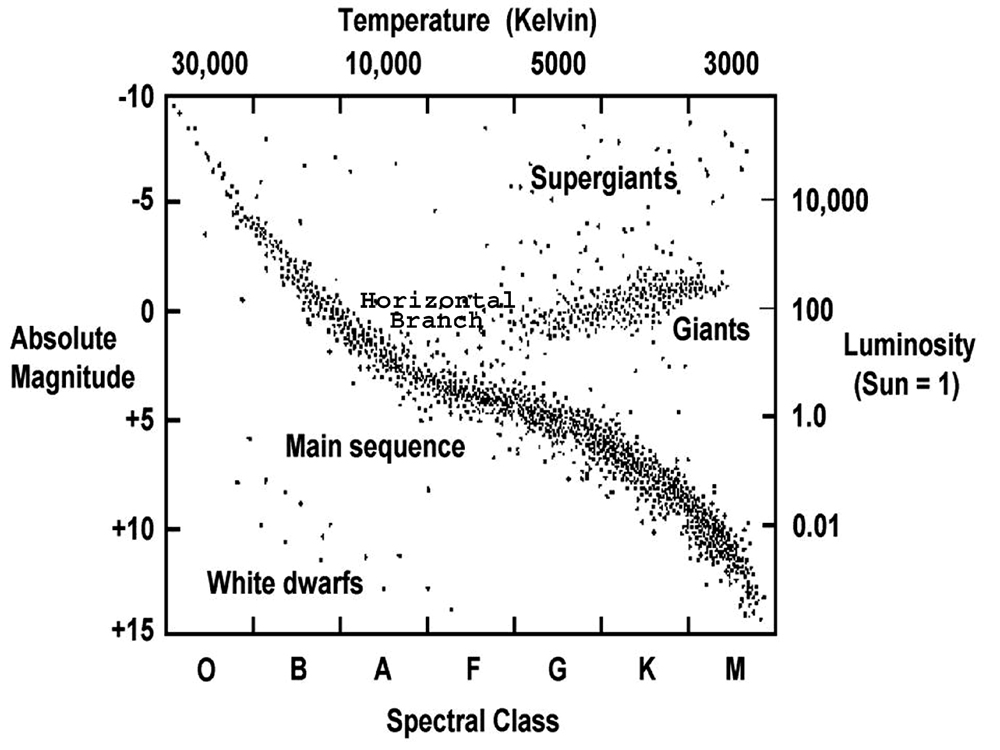
\includegraphics[width=2.5in]{fig/mainsequence.png}
% \caption{ Astronomers use  Hertzsprung-Russell diagrams to determine where is a star within the overall life-cycle of all stars.   Can we do something similar with software systems?}\label{fig:hr}
% \end{wrapfigure}
% By measuring, then mitigating, problems  in CSS software, this project will  enable all the 
% science that is discovered by that software.   Researchers into software
% analytics claim that there exists  
%   properties within all software projects that allows for the prediction
% of the future state of those projects. Like atoms in a star, these
% properties might be highly variable within any local context. 
% Nevertheless, if we step back to see the bigger picture, a pattern can emerge; e.g. see 
% Hertzsprung-Russell diagram of \fig{hr}. As with atoms, so too with software developers, If  we step back from the specifics of individual
% components, we can make predictions about large systems of individual developers.
%  But unlike stellar evolution,
% using the methods of this paper, developers and funding agencies can not only  predict 
% the current
% expected fate of a software project,  they can also take steps to 
% {\em change that fate}.

% % This project is somewhat different to a standard CSSI project. 
% % Instead of making predictions about physical phenomena,
% % in this work, we step back from that as say our ``phenomena''
% % being studied is the act of software development itself:

% % \begin{center}
% % {\em 
% % This proposal will make predictions about the   
% % process that  makes the software that enables computational science. 
% % \end{center}



% On the other hand,
% some CSS projects are not healthy and are ignored by the community
% (as witnessed by very little vigor or activity). To find, then fix,
% such projects, we apply methods from open source software to CSS projects.
% Those methods build models that offer
% accurate predictions on open source software project health,3,6,12,24 months into the future
% (where ``health'' is measured by values like number of closed pull requests and number of contributors).
% Those      methods have only been tested on software 
% that is ``market-driven''  (e.g. by   open source Silicon Valley industries) rather than ``science-driven''
% (e.g. by NSF funding cycles). Hence, here, we must test them   on computational science projects:
% \begin{formal}\noindent
% {\bf Goal1} of this project is to see how widely these health prediction methods apply to CSS projects.\newline
%  {\bf Goal2} of this project is to see if our predictors can be used to drive planners that propose
% useful changes to projects (where ``useful'' means ``improve project health'').
% \end{formal}
\noindent
Given the size of the CSS  community, our project improvement  goals
are  only widely applicable
if we can tame the data collection cost associated with this kind of analysis.  Outside of CSS
software,
{\em semi-supervised learning} has been used
to  restrain data collection to just the most informative examples. For non-CSS projects this
has meant  the effort associated with this kind of
study can be reduced by a factor of 40~\cite{tu2021frugal}\footnote{A core problem with analytics is ``labelling''; i.e. acquiring the ground truth associated with each example. Semi-supervised methods take a small number of labels then intelligently ``spread them round'' their nearest neighbors. In this way, Tu et al.~\cite{tu2021frugal} was able to reduce the labelling effort of their case study to just 2.5\% of the examples.}. 
But the value of that semi-supervised learning to
to CSS projects
has yet to be tested. Hence:
\begin{formal}\noindent
{\bf Goal3}: achieve Goal1,Goal2 for CSS projects via minimal data collection (discussed in \S\ref{goal3}).
\end{formal}
\noindent
Moving on to our next goal,
all this  research is   wasted {\em unless} it is applied
within the CSS community. Accordingly, our next goal must be:

\begin{formal}\noindent
{\bf Goal4}:  get our recommendations used by CSS community (discussed in \S\ref{goal4}).
\end{formal}
\noindent
For reasons of data availability, this proposal deals with CSS projects stored in the Github code repository.
By our counts, there are at least 700 such projects. But what about
other kinds of software?
\begin{formal}\noindent
  {\bf Goal5}:  apply our methods to CSS projects not stored in Github
  (discussed in \S\ref{goal5}).
\end{formal}
\noindent
Finally, we need one last goal:
\begin{formal}\noindent
 {\bf Goal6}:
find a set of general methods   for improving CSS projects (discussed in \S\ref{goal6}).
\end{formal}
\noindent
Technically speaking, {\bf Goal6} is a 
{\em transfer learning task}~\cite{KrishnaMF16,Nam13,Ma2012,jing15,Kocaguneli2014,yu2017feature,jamshidi2017transfer,pan2009survey,qing2015cross,li2018cost};
i.e.   lessons from one kind of project are   transferred
to another. 
As discussed in 
\S\ref{mm}, recently we had much success with hierarchical clustering algorithms that generate a handful of models  that apply to hundreds of conventional projects~\cite{majumder2019learning}. In  this proposal,
we would check if those methods work for CSS projects.
 
% The experience to date (with standard open source software~\cite{xia2020predicting}) is that while the prediction models are local to each project,    the method used to generate those models works for multiple projects.  That said, as discussed below, there is reason to suspect that it might be possible
% that CSS software is more regular that standard open source source. This means that it might be possible to learn general lessons for project health that apply to many CSS projects both within and without Github.
 
 
\section{Background}
\subsection{Frequently Asked Questions}
\noindent
 When discussing this proposal with colleagues, their first question is always:
 
 \begin{center}
 {\em FAQ1: are we trying to replace research scientists as they apply their creativity to computational science problems?} 
 \end{center} That is not the goal here.
 Instead,  {\IT} will explore  the software engineering decisions that can lead to
project success or failure.
 When we look at success stories for community-developed   software
 (e.g. the Apache Foundation or the Linux Foundation~\cite{apacheprojects,linuxprojects}), we find that the most successful software  projects
 are those  that attract  
 a large user base
 {\em and} a large funding base (where 3rd parties offer support for that code). While
 the funding support any one source   may be small,
 the combined funding   enables  the infrastructure needed for long-term viability.
 
 When attracting a funding base for a project,   the {\em reputation} of that project is very important. No one wants to fund a flailing or failing project. Hence,
 project health is often used to make the case 
 (e.g. to upper-management) that  some   software is worthy of funding.
A similar story can be told about how
 to attract developers to user your tools~\cite{xia21}. No
 one wants to based their work on some library
 that, in the near future, will be abandoned by its
 developers.  Perceptions of future  project health  of a project determines how many developers will be attracted to a project.
 
 Note that in both cases,   improving project health (via the methods of this proposal)  increases
 the probability that a project will become more sustainable (by attracting more
 funding and more developers).
  

Another questions we are often asked is:

\begin{center}
{\em FAQ2: what can be changed in a software project to make it better?}
\end{center}
Decades of research into software analytics by PI Menzies~\cite{menzies2016perspectives,menzies2018software,bird2015art,xia2019sequential,xia2020predicting,tu2020changing,tu2021mining,peng2021defect},
and others~\cite{kim2016emerging,buse2012information,amershi2019software,barry1981software}, shows that there are many  software project decisions that can make a project more (or less) attractive to other developers:
Some of these reasons are high-level
e.g.
\bi
\item
Choice of platform; using/avoiding unpopular dependencies; how the project interacts with the scientific developer community; choice of software license; numerous internal
architectural decisions; etc. 
\ei
Some of these reasons are much lower level; e.g.
\bi
\item
If a specific application programmer's interface
is tedious or complex to use, then external developers
will avoid this API, and perhaps even this entire CSS project.
\ei
In either case (low-level or high-level issues), {\IT}
will employ data mining on project data to:
\bi
\item Recognize a problem; e.g. recognize when the comments about an API are mostly negative;
\item
Propose a solution; e.g. recommend that the API be simplified.
\ei
Finally, we are often asked: 

\begin{center}{\em FAQ3: if {\IT} has already been developed, what is the core science of the problem being discussed here?}
\end{center}
In reply we say that parts of
{\IT} have only been tested only on general open source software, not CSS software. As discussed
below, these two kinds of software
are different enough to make it an open question if
{\IT} will work for CSS. 

As to the question about core science,
while {\bf Goal1, Goal4, Goal5} are case studies (where we apply  old {\IT} to new data), 
the other goals address core scientific issues
 relevant for any data mining problem:
 \bi
 \item {\bf Goal2}: Can our learners make any predictions about what to change in order to alter future outcomes?
\item {\bf Goal3}: Can we reduce the data sampling needed
to build an adequate model?
\item {\bf Goal6}: How general are our models (or must  we always reason over numerous different   models)?
\ei
\newpage
\subsection{Definitions}\label{distinct}
\noindent
Our premise is that Computational Science Software projects (CSS)
is very   
different to standard open source software (SOSS).
Hence, even thought we have preliminary results with {\IT} on SOSS code,
we can not assert that {\IT} will work on CSS software until we test it.

The next section offer empirical data on the   differences between CSS and SOSS. Before that, we offer some definitions:
\bi
\item {\em SOSS softxxware:} 
Conventional open-source projects are developed and distributed
for free redistribution~\cite{Raja12}. SOSS tools are widely used, even within the CSS community.
For our purposes, the major different between CSS and SOSS is the level of domain comprehension
seen in the developers.  While CSS developers have a deep understanding of the phenomena that
are explored, an SOSS developer can be anyone in the world with any level of domain training.

\item {\em CSS software:} Computational scientists explore software models than  
explore the physical effects. Exploring such models can be  faster, cheaper, and safer than exploring
the real world. For example, it is safer to explore models of hurricanes rather than the real thing.
For another example,
in material science, CSS explores the properties of new materials by
synthesizing them. Such synthesis can be very  expensive so standard practice
is to use software to cull the space of possibilities (e.g. via a finite
element analysis).  
A key feature of CSS software is that extensive background needed to understand, maintain and improve
this kind of software. For this reason, many CSS developers have advanced degrees in Physics, Chemistry, etc.  
Another difference is that 
 CSS code is developed more for science reasons rather than,  in the case of SOSS, to satisfy they whims of the developers or the vagaries
of the market place.
\ei


% While all this will be applied to computational science, the more general   point here is
% a comment on how huamns should investigate the work.  
% Brieman decribes two cluterures of statiscal anaysis of data: either assume an  apriori some distribution (and go hunt for it) or apply some open-ended data mining  method that hunts though a large space of possible
% models before decising which one might be approrpaite. It is an open 
% isse which approach is most prdocutive. Both approaches
% have their
% ardent supporters and detractors (e.g. the Google team lead by Norvig endorses ``open-ended''
% while Bayesians urge us to first define our apriori assumptions before doing any mining).
% This NSF proposal 





%XXXX bridge from here to other stuff 
\subsection{Results from Prior CSSI Projects}\label{prior}


The   section offers  empirical evidence
that CSS projects are fundamentally different to
SOSS projects.  These results come from a  prior  CSSI-funded    project\footnote{Elements: Can Empirical SE be Adapted to Computational Science?
Award \#1931425.  PI= Dr. Tim Menzies, NCState. 2019-2022.}.  The differences documented
in this section justify the core premise of this work: even if parts of {\IT} are known to work for standard software systems, we still need to check if it works for CSS code. 


 \begin{wraptable}{r}{1.5in}
\vspace{-5pt}
\centering
\caption{Project selection rules. From~\cite{Kalliamvakou:2014}.}\label{tbl:sanity}
\vspace{-5pt}
\footnotesize
\begin{tabular}{r|l}
 Check   & Condition    \\\hline
 \# Developers & $\geq$ 7 \\
 Pull requests  & $>$ 0 \\
Issues & $>$ 10 \\
Releases &  $>$ 1 \\
Commits & $>$ 20 \\
Duration  & $>$ 1 year 
\end{tabular}%}
\vspace{-10pt}
\end{wraptable} 
The following  study used (1)~a
 {\bf comparison set} of CSS and SOSS projects;
 (2)~a set of 
 {\bf project health indicators}.
In this   study, we
 compared 60 CSS projects to  1037 Github SOSS projects from~\cite{Majumder19}.
 We  use  project data from Github since this keeps data on CSS and both SOSS in a standardized way.
 
As to how we selected these SOSS projects,
the software analytics community
has long debated how to select ``interesting'' projects. Their standard ``sanity checks'' (used in this analysis) are shown in 
Table~\ref{tbl:sanity}.

As to our selection of CSS projects, 
we combined projects associated with a specific NSF grant and from   contacts in the CSS community
(from the Molecular Sciences Software Institute (MOLSSI) and the Science Gateways Community Institute (SGCI)).
Many of these were single-person projects (e.g.   ``glue'' projects from the Gateway). While those kinds of projects are an important part of the CSS community, in terms of number of developers, we find that that we can cover far more developers by applying the Table~\ref{tbl:sanity} sanity checks to that sample of CSS projects.
 

  These CSS and SOSS projects were compared using the following   health indicators:
\be
\item \textit{Developers}: are the active contributors to a project.
% , who code and submit their code using commit to the code base. The number of developers signifies the interest of developers in actively participating in the project and volume of the work.
  
  

\item \textit{Commits:} adds the latest source code to the repository.
% in version control systems, a commit adds the latest changes to the source code to the repository, making these changes part of the head revision of the repository. 

\item  \textit{Open \& Closed Issues:} are used to track ideas, enhancements, tasks, or bugs.

% users and developers of a repository on Github use issues as a place to track ideas, enhancements, tasks, or bugs. As they work, they open issues with Github. When developers address those matters, they close the issues.

\item  \textit{Tags}: are references that point to a specific time in the Git version control history. 
%Tagging is generally used for marking version release (i.e., v1.0.1).


\item  \textit{Releases:} are different versions published (and  signifies a considerable  change between each version)
% mark a specific point in the repository’s history. The number of releases defines different versions published (and  signifies a considerable  change between each version).

\item \textit{Duration:} length of the project from its inception to the current date or project archive date (in weeks).
%of a project marks the length of the project from its inception to the current date or project archive date (in week as a unit of time). It signifies how long a project has been running and in the active development phase.
\item \textit{Stars:}  people who
  ``liked'' a project's repository (and bookmarked it to get updates on   future progress.)
  
\item   \textit{Forks}: how many people are interested in the repository to make a copy of it while  allowing users to freely experiment without affecting the original project.
   
   % Forking a repository allows users to freely experiment with changes without affecting the original project. 
   % This number is an indicator of how many people are interested in the repository and actively thinking of modification of the original version.
  
\item   \textit{Watchers}:  Github users asking to be notified of repository activity, but have not become collaborators. 
   % This is a representative of people actively monitoring projects, because of possible interest or dependency.
\ee
Note that some of these indicators are more insightful than others. ``Stars'', for example, is more a popularity contest than a deep semantic dive into a system. On the other hand, ``number of closed issues'' is a core measure  revealing who cares enough about   code to recompile it and fight with its errors.
 
 
% \begin{wraptable}{r}{1.5in}
% \vspace{-15pt}
% \caption{Languages in 59 CSc projects.  
% }\label{tbl:language}
% \vspace{-12pt}
%  \footnotesize
% %\begin{threeparttable}
% %\vspace{-10pt}
% %\resizebox{!}{0.2\linewidth}{
% %\setlength        abcolsep{10pt}
%  \hspace{-3pt}\begin{tabular}{l|c|c}
%  \multicolumn{1}{c|}{} & \multicolumn{1}{c|}{Count} & \multicolumn{1}{c}{Percent}\\
% \hline
% Other & 3 &  5\%  \\ 
% Javascript	& 2 & 3\% \\ 
% C &	3 & 5\% \\ 
% Java	& 5 & 9\% \\ 
% Fortran	& 6 & 10\% \\
% C++	& 17 & 29\% \\
% Python & 23 & 39\% 
% \end{tabular}
% \vspace{-10pt}
% %}
% %\end{threeparttable}
% \end{wraptable}
\fig{health} compares these indicators for CSS and SOSS projects.
 Based on  a combination of
  a 95\% confidence bootstrap statistical test~\cite{efron94} and an A12 effect size test~\cite{arcuri2011practical}, we offer the following notes:
  \bi
  \item Both projects have similar number of
  developers per project;
  \item
CSS  projects have a shorter  median {\em duration} 
than SOSS projects   (281 weeks versus 409 weeks);
\item Interestingly, in that time, the CSS projects
  (a)~make more commits and (b)~close many more issues and (c)~make many more releases.
  \item
  That is to say, at least in this sample, CSS projects
complete more work with the same number of people in 
signficantly less time than    SOSS projects.
  \ei 
\begin{figure}[!b]
~~~~~~~~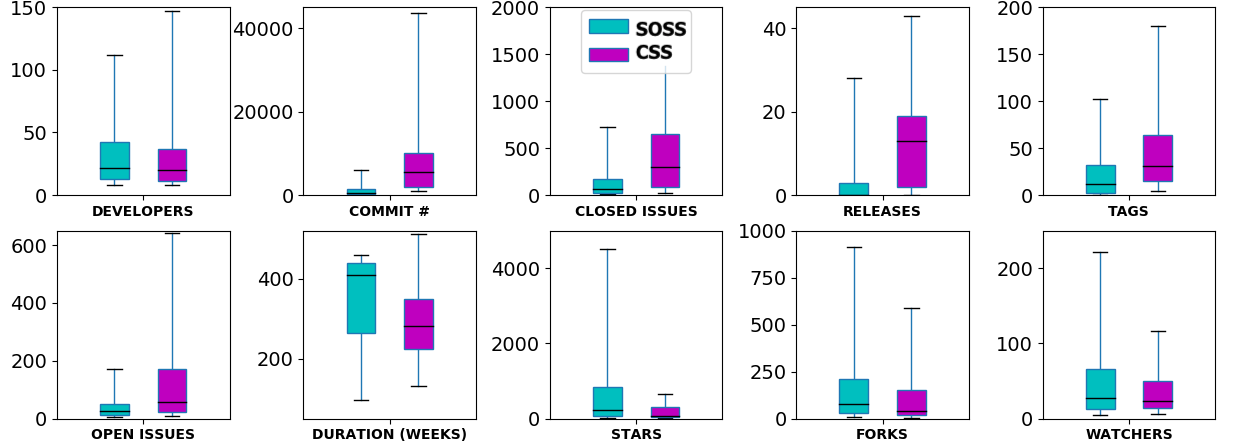
\includegraphics[width=5.7in]{fig/compare.png}
\caption{
Standard open source projects are shown in turquoise

\includegraphics[height=2mm,width=5mm]{fig/SOSS.png}.
Computational science software projects are shown in  purple

\includegraphics[height=2mm,width=5mm]{fig/CSS.png}.
 By all these health indicators, the following
CSS projects are better than SOSS:
{\em ABINIT,
AMBER,
APBS,
BLIS,
GooFit,
HooMD-blue,
LAMMPS,
LIBMESH,
Luigi,
MADNESS,
MDAnalysis,
MPQC,
NWChem,
OpenMPI,
OpenMX,
OpenMm,
PCMSolver,
PLUMED,
Psi4,
RMG-Py,
SCIRun,
TRILINOS,
TauDEM,
Use,
Xenon,
abaco,
cctools,
changa,
cyclus,
dealii,
elasticsearch,
forcebalance,
foyer,
hydroshare,
irods,
learnsphere,
mast,
mdtraj,
metpy,
openforcefield,
openmmtools,
orca,
parsl,
pymatgen,
pyscf,
quantum\_package,
radical-pilot,
signac,
signac-flow,
trellis,
yank,
yt}.
}\label{fig:health}
\end{figure}
% \fig{health} is not our only evidence that of the robust
% health of many CSS software. Many writers
% such as  Basili, and others~\cite{basili08_hpc, carver07_environment, Prabhu11_cssurvey, kendall05_C, ragan14_pythoncs,faulk09_secs,sanders08_risk,Prabhu11_cssurvey} express are concerned that CSS projects
% are using older tools (Fortran is often mentioned).
% To test if CSS software is  using out-moded tools, we counted  what were the main languages in our CSS sample.
% This test assumes that if CSS teams are mostly focused on ``old'' technology then most of those projects would use ``old'' languages and would not use automated testing
% tools such as  Travis CI\footnote{Travis
% CI is an automatic testing facility that is often run from Github.
% From {\em Wikidpedia}: When Travis CI has been activated for a given repository, GitHub will notify it whenever new commits are pushed to that repository or a pull request is submitted.  Travis CI will then check out the relevant branch and run the commands specified in the  .travis.yml file, which usually build the software and run any automated tests. When that process has completed, Travis notifies the developer(s).}
% The results of this ``are they using newer technology?'' test are shown in \tbl{language}.
% As seen there,  C and Fortran are just 15\% of our sample.
% Even if we call C++ ``old''\footnote{
% Johanson et al.~\cite{johan18_secs} say that, in CSS, Fortran and C are examples of this ``old'' technology. The use of C++ is an interesting borderline case- Johanson et al. regard that as ``new technology'' even though it is now decades old. In any case, C++ is not a part of the \fig{language} results.}, then the ``older'' technologies of \tnl{language}
% cover less than half the sample (44\%).
% As to other measures of ``new'', we find that  $43/59=73\%$
% have active
% Travis CI connections. 
% %We also observe some other SE methods and technologies include \textit{YT}~\cite{yt_project} and  \textit{AMBER}~\cite{Amber-MD} employ Docker~\cite{DOCKER} to simplify applications deployment,  \textit{LAMMPS}~\cite{lammps-sandia} and \textit{DEALII}~\cite{BangerthHartmannKanschat2007} can run on parallel processors, \textit{PSI4}~\cite{psi4} and \textit{XENON}~\cite{xenon} to test   code coverage. 
One way to summarize the above is that:
 
 
  \begin{center}
  {\em Computational science projects are performing much  better than standard SOSS
projects.} 
  \end{center}
This result is at odds with  prior work~\cite{basili08_hpc, carver07_environment, Prabhu11_cssurvey, kendall05_C, ragan14_pythoncs,segal_enduser,  carver13_perception, sanders08_risk} that complains that  CSS software is somehow
problematic:
\bi
\item
Basili et al., and others~\cite{basili08_hpc, carver07_environment, Prabhu11_cssurvey, kendall05_C, ragan14_pythoncs} say that
computational scientists prefer
``older''-style programming languages and technologies (and disregard most of the newer SE methods). To that, we would reply that even if they are using supposedly older tools, 
\fig{health} suggests CSS developers are using those tools very effectively. 
\item
Segal~\cite{segal_enduser},
and others~\cite{basili08_hpc, carver13_perception, sanders08_risk} comment that  few CSS scientists are trained in SE.  This is concerning as a lack of training might lead to sub-optimal software
development
 (for many of these people,
learning SE is perceived as an excessive additional burden~\cite{boyle09_lessons}).
To this concern we would reply that however they are trained, 
\fig{health} suggests that CSS developers are
using that training very effectively.
\ei
% % Before we list those widely-held beliefs, we stress that our research
% % suggests that the following beliefs
% % are \underline{\bf NOT} true (at least, for the CSS software we examined in Github):
% % \bi
% % \item
% % {\em Belief1: CSS developers have
% % old tools.}
% % According to this belief, CSS software uses old,
% % and possibly sub-optimal and out-dated, methods.
% % For example,
% % The usual argument here is that CSc Scientists are skeptical of modern SE methods and new technologies/languages.
% % This is based on several factors such as
% % (a)~a prejudice against  newer languages;
% % (b)~a perception that CSS developers would not 
% %   find new tools very  useful~\cite{Prabhu11_cssurvey};
% %   (c)~a decades-long commitment to  older-style languages (Fortran \& C)~\cite{faulk09_secs}.
% % (d)~a  belief that the extra features of the newer languages needlessly conflate functionality that can be more easily implemented in, e.g., one line of ``C'' macros~\cite{sanders08_risk}; 
% % \item
% % {\em Belief2: CSS developers have  the wrong skills,
% % and may not even want to learn new ones.}
% % CSS software is worse that other
% % code, it is said,  since it is built
% % by people not trained in up-to-date methods.
% % For example,   
% \ei
% Neither of these beliefs are supported by our results.
% The discussion around \tbl{language} found not evidence of a preponderance of older technology. Further,
% the results of \fig{health}, CSS projects are delivering and maintaining more software in less time with fewer developers than SOSS projects. 
To explain this discrepancy between
the optimism of \fig{health}
and the pessimism of Segal, Basili
and others~\cite{basili08_hpc, carver07_environment, Prabhu11_cssurvey, kendall05_C, ragan14_pythoncs,segal_enduser,  carver13_perception, sanders08_risk}, 
we offer three notes:\bi
\item
Software development is certainly difficult.
Hence, Segal, Basili
and others are certainly correct in warning the CSS software development is difficult. That said,
by asking a slightly different question, we arrive a new perspective not previously reported. Instead of asking
``Q1) is CSS code development difficult?'', we   ask instead ``Q2) is CSS code development
{\em comparatively more difficult} than
other kinds of software?''. And as \fig{health} shows us, the answer to Q2 is ``no''.
\item
Most of the papers lamenting the state of CSS code come from before the recent Silicon Valley boom. In our recent discussions with postdocs and Ph.D. students working on CSS projects,
we found that these developers were well aware of the potential salaries if they are adept at the popular tools used by contemporary agile software companies.
Hence we suggest that something of a ``phase change'' has come over
CSS software and that newer codes should be expected to be somewhat more
better than past offerings.
\item
When computational scientists developers write CSS code, they are exploring domains with  an extensive background theory (all the physics and chemistry achieved in thousands of years of scientific research).  When other developers write code
about (e.g.) database systems, they are writing about domains with only a few decades
of theory.  Also, CSS developers typically have multiple degrees, some even with higher degrees. Conventional software authors, on the other hand, many have a far less
scientific training. When stated this way, it is hardly surprising that developers with more scientific working over a  richer background theory generate better systems than otherwise.
\ei
\subsection{Measuring and Mitigating Project Health Issues}\label{mm}
 \begin{wraptable}{r}{3in}
 \begin{adjustbox}{max width=3in}
 \begin{tabular}{l|rrrrrr}
\multicolumn{7}{c}{ error =  MRE =  $\mathit{abs}(\mathit{predicted} - \mathit{actual})/\mathit{actual}$ (so {\em less} is {\em better})   }\\\hline
\rowcolor[HTML]{ECF4FF} 

{\cellcolor[HTML]{FFFFFF} predicting for:} & {\color[HTML]{000000} KNN} & {\color[HTML]{000000} LNR} & {\color[HTML]{000000} SVR} & {\color[HTML]{000000} RF} & {\color[HTML]{000000} CART} & {\color[HTML]{000000} DECART} \\\hline
{\color[HTML]{000000}   \#commits} & \cellcolor[HTML]{E2E2E2}53\% & \cellcolor[HTML]{F3F3F3}107\% & \cellcolor[HTML]{E9E9E9}68\% & \cellcolor[HTML]{E1E1E1}53\% & \cellcolor[HTML]{E2E2E2}52\% & \cellcolor[HTML]{DCDCDC}41\% \\
{\color[HTML]{000000}   \#contributors} & \cellcolor[HTML]{CACACA}32\% & \cellcolor[HTML]{9F9F9F}26\% & \cellcolor[HTML]{D9D9D9}35\% & \cellcolor[HTML]{898989}24\% & \cellcolor[HTML]{989898}24\% & \cellcolor[HTML]{666666}\textcolor{white}{18\%} \\
{\color[HTML]{000000}    \#stars} & \cellcolor[HTML]{BFBFBF}30\% & \cellcolor[HTML]{D9D9D9}35\% & \cellcolor[HTML]{D9D9D9}36\% & \cellcolor[HTML]{B9B9B9}30\% & \cellcolor[HTML]{DADADA}37\% & \cellcolor[HTML]{9F9F9F}26\% \\
{\color[HTML]{000000}  \#open issues} & \cellcolor[HTML]{D9D9D9}36\% & \cellcolor[HTML]{DEDEDE}45\% & \cellcolor[HTML]{DBDBDB}39\% & \cellcolor[HTML]{D9D9D9}34\% & \cellcolor[HTML]{C3C3C3}31\% & \cellcolor[HTML]{8C8C8C}23\% \\
{\color[HTML]{000000}   \#closed issues} & \cellcolor[HTML]{DCDCDC}41\% & \cellcolor[HTML]{B5B5B5}29\% & \cellcolor[HTML]{DDDDDD}44\% & \cellcolor[HTML]{ADADAD}28\% & \cellcolor[HTML]{CACACA}32\% & \cellcolor[HTML]{828282}22\% \\
{\color[HTML]{000000}   \#closed pull requests} & \cellcolor[HTML]{DADADA}38\% & \cellcolor[HTML]{DBDBDB}39\% & \cellcolor[HTML]{DBDBDB}40\% & \cellcolor[HTML]{DEDEDE}44\% & \cellcolor[HTML]{DCDCDC}41\% & \cellcolor[HTML]{C3C3C3}31\%
\end{tabular} 
\end{adjustbox}   
\caption{Predicting project health. Median errors  in  1,159 SOSS projects~\cite{xia2020predicting}.  Darker cells=less
error. 
Lowest errors from ``DECART''. }\label{tbl:med_mre}
\end{wraptable}
Software development can be hard. Even if \fig{health} shows that CSS projects
might be relatively stronger than SOSS projects, there are still all-to-many examples
of NSF-funded CSSI projects that failed, or fell into disrepute, or have been ignored
by the rest of the community.
To fix that problem this section describes  methods to {\em find}, then {\em fix}
a failing project. 

Just to be clear, {\em none} of the material in this section
have yet been applied to CSS projects. The methods of this section would need 
significant extension to achieve the goals listed in the introduction. In the {\em next} section  of this proposal,
we addresses how we would test, then adapt,
these methods for CSS projects.
 
PI Menzies' prior work with generating health predictors (for non-CSS software)
was reported in~\cite{xia2019sequential,xia2020predicting}. 
In that report it was noted that numerous research had studied
project health~\cite{jansen2014measuring,manikas2013reviewing,chaoss,weber2014makes,borges2016predicting,wang2018will,bao2019large,kikas2016using,jarczyk2018surgical,qi2017software,chen2014predicting}. PI Menzies found numerous shortcomings with that
prior work:
\bi
\item That prior work usually studied a very small number of projects (perhaps, just even one);
\item That prior work usually explored a small number of indicators
(often, only one);
\item That prior work did not explore a range of learner methods;
\item That prior work did not apply tuning methods to automatically infer the best learner control parameters.
\ei
% For example,
% the CART regression tree learner has hyperparameters:
% \bi
% \item 
% max\_features: number of features to consider when looking for the best split;
% \item 
% max\_depth:   maximum depth of the learned tree;
% \item 
% min\-sample-leaf: minimum samples required to be at a leaf node
% \item
% min\_sample\_split: minimum samples required to split internal node
% \ei
 







~To address those issues, PI Menzies (and his student
Mr. Tianpei  Xia) applied their DECART tool to a wide range 
of projects~\cite{xia2020predicting}. DECART is  a recursive entropy learner 
tuned by 
a hyperparameter optimizer~\cite{storn1997differential}. PI Menzies tested DECART on
1100+ Gitub projects to
explore seven health indicators. In the study,
DECART was compared to five different learners (linear regression, CART, random forests, k-nearest neighbor, and support vector regression). It was found that:
\bi
\item
The right-hand-side column of  \tbl{med_mre}  
shows that DECART's errors
($abs(want\;-\;got)/want$)
are much lower than the other studied methods.
 These results     are 
 unexpectedly accurate.
Prior experiment with effort estimation had generated predictions
 with error ranging up to 200\%~\cite{kocaguneli2012value}.
 Hence our  pre-experimental expectation was that  these
 prediction errors would be up to ten times larger than what is seen in the right-hand-side
 column of \tbl{med_mre}.
\item
We have repeated the \tbl{med_mre} analysis for predictions up to two years into the futre.
The prediction error was observed to increase, but not by very much  (as little as 5 to 10\% more).
\ei
In summary,   these predictions are hence accurate enough to predict medium-term trends in a project (at
least for the SOSS projects studied here).  
 
\definecolor{aoenglish}{rgb}{0.0, 0.5, 0.0}
 \definecolor{applegreen}{rgb}{0.74, 0.85, 0.75}


That said, \tbl{med_mre} is more a 
{\em starting point} than a {\em conclusion}.
All these results are from SOSS project so,
without further testing,
it is unclear if these methods   work on CSS projects.
Also,   once we can predict for  $X$,
then the next question to ask is 
``how can we improve $X$''?  

To address that issue for (non-CSS) projects, PI Menzies
and his student Mr. Kewen Peng made several  observations~\cite{peng2021defect}.
 {\bf FIRSTLY}, the delta $\Delta$
between two regions of the data is
a candidate {\em plan} for moving from
more region to another. For example, consider the defect prediction
regression tree of \fig{XTREE}.
Each branch of that tree a logical conjunction.
To create a plan that changes a project from
(e.g.) a defective 
  \textcolor{orange}{{\bf current branch}}  to a better
 \textcolor{aoenglish}{{\bf desired branch}}, we can apply the 
$\Delta$ between the two branches. In the case of the example of
\fig{XTREE}, plan is to   minimize two static code attributes {\em lcom} and {\em cam}.  Such values can be changed via {\em software refactoring operators}
such as ``fold a sub-class into a superclass''; or ``push down a super-class method into 
the children''.



{\bf SECONDLY},  the models generated  by DECART (that lead to  \tbl{med_mre}) are of the same  form as \fig{XTREE}.
\begin{wrapfigure}{r}{3in}
   \includegraphics[width=3in]{fig/XTREE_samp.pdf} 
    \caption{  A {\em plan}
     is the delta $\Delta$
     that moves a project from the defective  \textcolor{orange}{{\bf current branch}}
    (where defect probability  is 1.00)  to another
     \textcolor{aoenglish}{{\bf desired branch}} (with zero defects).}
    \label{fig:XTREE}
\end{wrapfigure}
That, is DECART could be a front-end to a project planning process.
Note that
this  planning process that could be applied to    any model that comments on projects process or project attributes that tend towards  better/worst results (i.e. to more than merely the static code attributes of \fig{XTREE}).
 
 




~{\bf THIRDLY},   it is important to check the plans found in this way. Such plans  are hardly causal determinants of behaviour  
(causality is  precisely defined--    a single counterexample can refute the causal claim~\cite{AAAI_1990}). 
These  plans  have some likelihood (but no certainty) that they will work in the
way predicted for future projects. Hence, this kind of plan generation has to be paired with some {\em sanity check}
that prunes bad plans. 
Accordingly,
Menzies and Peng~\cite{peng2021defect}
used a {\em precedence sanity check} to only endorse  plans that proposed changes found in the historical record of a project. They found
that plans found in this way were much smaller than those proposed
by prior state-of-the-art mechanisms;
and just as effective (and sometimes better) than that prior work.
To assess that effectiveness, Menzies and Peng ran the
following \underline{\bf a,b,c what-if procedure} queries
across the historical
\label{abc}
log of a software projects.
This procedure takes project information divided into 
{\em oldest}, {\em  newer}, and {\em most recent} data, then:
\bi
\item[a.] Use the {\em oldest} data to determine what attributes were often changed in a project,
\item[b.] Use the {\em newer} data to build plans;
\item[c.] Divide the {\em most recent}  data into (i)~those projects that {\em follow}ed the plans;
 and (ii)~{\em other}.
\ei
They then found that  the {\em follow}ing
set had far better outcomes (lower defects) than 
the {\em other}s~\cite{peng2021defect}.
That is, if those plans had been available to developers, and they had applied them,
then a large number of the projects in the {\em follow}ing set would have the predicted outcome.

 \section{Research Plan}
 
 The above results showed that for non-CSS projects, it is possible to make predictions about the future
 health of a software project, then propose effective plans to improve that future state.
 The rest of this proposal discusses ways to test if the above methods apply to CSS projects.
 
In the following,
 {\bf  Goals1,2} are ``preliminary'' work with a few sample projects
and {\bf Goal3} is where we will attempt to scale up these methods. {\bf Goal4} 
is where we check the effect of the scale up and {\bf Goal5} is an opportunistic goal to handle
certain special cases not handled by {\bf Goals1,2,3,4}. Finally, {\bf Goal6} is an overview
on all the results seen in this work
(and in that part of this work, we will look for
a small number of general models).



  
 \subsection{Research Goal1:  predict   project health for  some   CSS projects}\label{goal1}

Currently, we know of around 700 CSS projects within Github. For a sample 
of those projects, we will apply the above methods to generate predictions for the nine
health indicators of \S\ref{prior} (on page \pageref{prior}).

\textcolor{red}{{\bf Measurable Outcomes:}}
We would generate the \tbl{med_mre}
error measurements,  but for CSS
projects.  Saro et al.~\cite{sarro2016multi} comments that for software project management, these errors should be less than 25 to 50\%. Hence we would say {\bf Goal1}
is achieved if we can make low predictions with that kind of error.



\subsection{Research Goal2: 
plan effective improvements for   some CSS projects}\label{goal2}

\noindent
This proposal seeks improvement
tactics for CSS projects that (a)~are generally useful (and cover many projects);
(b)~yet also sufficiently powerful for specific projects.
Currently, we know   
  five  such  tactics:
\be
\item The {\bf planning algorithm} shown above: This
 could be applied to a wide range of attributes or goals.
\item Those plans could be used to improve the 
{\bf nine    project health indicators} of \S\ref{prior} (or, indeed, any other effect recorded in Github data).
\item
{\bf Sentiment analysis}: This is a particular kind of data mining tool that looks at thousands to millions of code comments and infer where in the code base developers or users are have the most difficulty. Such tools can be applied to very large code bases to find regions that need the most rework.
For an example of source code sentiment analysis, see Table~\ref{source}. PI Menzies and his students have much
recent success with identifying one particular kind of sentiment: {\em self-admitted technical debt}~\cite{zhesatd20}.
When developers cut corners and make haste to rush out code, that
code often contains technical debt (TD), i.e. decisions that must be
repaid, later on, with further work. Technical debt is like dirt in the
gears of software production. As TD accumulates, development
becomes harder and slower. Technical debt is often ``self-admitted'' by the developer in code comments~\cite{Potdar14}; e.g. Potdar and Shihab~\cite{Potdar14} concluded that developers intentionally leave traces of TD in their comments (saying things
like ``hack, fixme, is problematic, this isn’t very solid, probably a
bug, hope everything will work, fix this crap'').
That said, these self-admitted problems are often lost in
the rush to finish a release. Nugroho et al.~\cite{Nugroho11} report that medium-sized projects can carry around so enough technical debt
to significantly delay  enhancements and maintenance.
PI Menzies and his student Dr. Zhe Yu found they could
improve on current automated solutions  for identifying SATDs 
using a two-stage approach (where stage1 used simple methods
to find majority of simple SATD problems and stage2 used
much more complex methods to resolve the residual issues)~\cite{zhesatd20}. 
\item {\bf Automatic tuning methods}:  Many software systems come with configuration options; 
\bi
\item
e.g. 20 binary options means over a million possible configurations. 
\item
e.g. the Makefile of MySql has over a billion possible different configurations;
\item 
e.g. data miners are controlled by a large number of hyperparameters. Nearest neighbor methods, for example, need to know (a)~how many nearest neighbors to explore and 
(b)~how to to combine the information from those neighbors.
\ei
Automatic configuration tools can find configurations that are much better than those set by humans~\cite{Xu15a,shu2019improved,xia2019sequential,agrawal2018better,fu2016tuning,agrawal2018wrong,spike_jc_19,xia2018hyperparameter,chakraborty2019software,nair2017using}.
PI Menzies and his students have much recent success with building very fast, very scalable automatic tuning methods~\cite{agrawal18,flash_vivek,tu2021mining}
Table~\ref{casestudy} reports a case
study we successfully applied this
optimization technology to improve workflows from the  Pegasus Research group. 
\item
{\bf Automatic AI-based code  recommender systems:} Given a very large corpus, neural networks can learn expected words in a program. Such tools can peek at a few terms written by a programmer, then comment on what needs to come next in that code. Examples of these kinds of tools include Codex, Copilot, TabNine, Kite and Facebook's SapFix~\cite{codex,sapfix,xu-ide}.
\ee
\begin{table}[!t] 
\caption{Sentiment analysis   finds code   disliked by developers (that deserves improvement). From~\cite{Guzman14}.}\label{source}
\footnotesize
\begin{tabular}{p{2in}p{3.5in}p}\\\hline
Commit message &Word and sentence score& Total
score\\\hline
Sigh? It’s fixed, man – rejoice!! & Sigh?[sentence: 1,-1] It’s fixed ,man –rejoice[4]!![+1 punctuation emphasis]
[sentence: 5,-1]
&
5\\

% Wow amazing thread! even If I’m not a Rails
% developer!&
% Wow[3] amazing[3] [+1 consecutive positive words] thread![+1 punctuation
% emphasis] [sentence: 5,-1] even If I’m not a Rails developer ![+1 punctuation
% mood emphasis] [sentence: 2,-1]
% &
% 5\\
MY PRECIOUSSS!!! & MY PRECIOUSSS[3] [+0.6 spelling emphasis] !!![+1 punctuation emphasis]
[sentence: 5,-1]&
5
\\
If PHP code is producing errors with register globals on you are terrible terrible programmer. If you are using magic quotes you are
simply stupid.  &
If PHP code is producing errors[-2] with register globals on you are terrible[-4]
terrible[-4] [-1 consecutive negative words] programmer.[sentence: 1,-5] If you
are using magic quotes you are simply stupid[-3].[sentence: 1,-3]
&

-5\\
% % But this commit message makes me sad :cry: &But this commit message makes me sad[-4] :cry[-4] [-1 consecutive negative
% % words] :[sentence: 1,-5]&
% % -5\\
% This is really terrible - changing :private to
% :public without any deprecation warning? Not
% cool. &
% This is really terrible[-4] [-1 booster word] -changing :private to :public without
% any deprecation warning?[sentence: 1,-5] Not cool[2] [*-0.5 approx. negated
% multiplier] [sentence: 1,-5].&
% -5\\
\hline
\end{tabular}
\end{table}\begin{table}[!t]
\caption{Automatic tuning methods improving workflows for the  Pegasus Research group and Renaissance Computing Institute at UNC (RENCI). From~\cite{tu2021mining}. }\label{casestudy}
\small
\begin{tabular}{|p{.98\linewidth}|}\hline
Orchestrating and managing data movements for scientific workflows within and across   diverse infrastructures  is challenging~\cite{taylor14_workflows}. The problem is exacerbated by different kinds of failures and anomalies that can span all levels of such highly distributed infrastructures (hardware infrastructure, system software, middleware, networks, applications and workflows). Such failures add extra overheads to scientists that forestall or completely obstruct their research endeavors or scientific breakthrough.
At the time of this writing, these problems are particularly acute (the COVID-19 pandemic has stretched the resources used to monitor, maintain and repair the infrastructure).
  As shown here by the red dots, network traffic can spike, denoting periods of time where a site cannot handle all the incoming traffic (this data comes from RENCI-- 
   the   Renaissance Computing Institute at UNC): 
\begin{center}
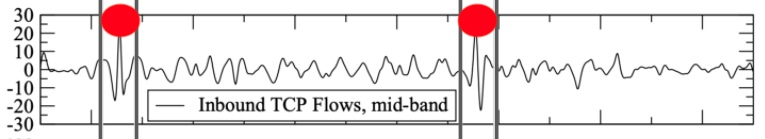
\includegraphics[width=4in]{fig/spike.jpg}
\end{center} 
All previous anomaly detection work in scientific workflow lacks (i) model optimization and (ii) a tuning study.  This is hardly ideal since much prior work    advises that using data miners without  parameter optimizer leads to sub-optimal results~\cite{agrawal18, fu2016tuning, spike_jc_19}.
PI Menzies and Mr Tu showed that for workflows seen at the Pegasus research group,   
standard anomalies learning tools for faulty TCP file transfers (without tuning) can be considered \textit{harmful} and \textit{misleading} to the reliability of networked infrastructures~\cite{tu2021mining}. 
%Among the cyberinfrastrucutre, such anomalies may change the experimental results that lead to scientific progress can be forestalled and discovery results can be even refuted.
Their proposed improvement utilized better data mining methods; specifically,
 an ensemble model (XGBoost~\cite{xgboost}) and a sequential model-based tuner (FLASH~\cite{flash_vivek}). They found that
\bi 
\item Tuning  learners will improve the relative performance up to 28\%, 29\%, and 40\% for F-measure, G-score, and recall   from the prior state-of-the-art  work~\cite{tcp_indis_19}. 
\item Tuning changes previous conclusions on what learner is the best performing, i.e., from random
forests (as recommended by prior work) to XGBoost (recommended by this work).

\item Tuning changes previous conclusions on what  factors are most
influential in detecting for anomalies by 30\%. That is, a side-effect of this work
is that it is time to change what we monitor for. 
\ei
  \\\hline
 \end{tabular}
  \end{table}
Computational considerations suggest that, of the above five tactics, we will be able to apply Tactics1,2,3 more often than Tactics4,5.
Tactics1,2,3 are data mining methods that can easily scale-up
to many   projects. Tactic4 is slower since, for each project,
it must re-run the learners hundreds to millions
of times (to learn the best tunings for that project). Lastly, Tactic5 might be slowest of all since it could
require  pre-training a neural net of  a very large corpus of CSS code.

 \label{tactics2}
\textcolor{red}{{\bf Measurable Outcomes:}} For   tactics 1,2,3 we can assess the results of our interventions using the  
    {\bf a,b,c what-if procedure} defined   at the end
of \S\ref{mm}
(on page \pageref{abc}). Also, for tactic3's self-admitted technical debt, 
if we   track the levels of technical debt in a project (using our data miners) 
and the metrics
of \fig{health}, then
then we can detect if our
technical debt reductions are having benefits within a projects.
As to tactics4,5 the outcomes we want to measure would need to be tuned to specific systems we are tuning or 
for which we are generating recommendations. 
 
 


\subsection{Research Goal3:  achieve Goal1,Goal2 via   minimal data collection}\label{goal3}

Given the size of the CSS community, the above goals may only be widely applicable if we can tame the data
collection cost associated with this kind of analysis.  
To understand that collection cost, we note
that any data miner uses large databases of $x,y$ examples to generates a model
$f$ of the form:
\[
y=f(x)
\]
Here, $x$ is project information 
(such as lines of code, number of recent updates, number of developers, etc) and $y$ is information about project performance (such as the ease of use of this code, the penetration of this code, the cost of developing the code).
Given access to Github, it is now possible to automatically collect $x$ data fro a very large number of projects. However, collection accurate $y$ is another matter.
Even when projects offer $x,y$ data, the $y$ labels
are often questionable. 
For example,  Yu et al. checked the $y$ labels
 (about software defects)
 from one Github project and
 found that more than 98\% of
the false positives (reported by prior work) were actually true positives, casting doubt on
work that used the original dataset~\cite{jitterbug}.
PI Menzies' graduate student Mr. Huy Tu~\cite{tu2019better} has developed cost models describing the effect required to check these $y$ labels where:
\bi
\item
Data is checked by pairs  of web-based crowd-sourced  workers using the Amazon Mechanical Turk facility (so results are not accepted unless two people
 agree on the label).
\item
The crowdworkers are assessed by questions with known answers (so we can prune unreliable  workers).
\ei
According to the Tu model,   it would take 
200,000 hours and cost \$2,100,000 to  review the $y$ values related
to known defects in the $\approx 700$ CSS projects we can find in Github. 

To say the least, such large costs
are   unacceptable.
Hence, Mr. Tu went on    to investigate
{\em semi-supervised methods} for reducing the cost associated with labelling Github data.
Working with non-CSS data, Mr Tu found that he could build effective software quality prediction models
by labelling just 2.5\% of the data~\cite{tu21Frugal}. Note that a 2.5\% reduction   reduces that \$2,100,000 to \$52,500 which, is spread out of a three year NSF projects becomes more acceptable at \$17,500 per year (a much more reasonable sum). 

For a brief tutorial on semi-supervised learning, see Table~\ref{inside}.
Note that none of those methods have yet to be  tested on CSS software. Nor have they been used
when trying to achieve {\bf Goal1,Goal2}. Hence...


\textcolor{red}{{\bf Measurable Outcomes:}} To test the effectiveness of semi-supervised 
learning for reasoning about CSS projects, we would generate ``trade-off graphs''
where we repeat the analysis of {\bf Goal1, Goal2} using fewer and fewer
$y$ levels (selected by  semi-supervised learning). {\bf Goal3} would be declared achievable
if we can achieve competency for {\bf Goal1, Goal2} after labelling 2.5\% (or less) of the
data.
\begin{table}[!t]
  \caption{A brief tutorial on semi-supervised learners 
}\label{inside}
 \small
 \begin{tabular}{|p{6.35in}|}\hline
 
 {\em Semi-supervised learners}~\cite{mit06}  train their models by
combining a small amount of labeled data ($Y$ values) with a large amount of unlabeled data ($X$ values).
More specifically, 
  semi-supervised algorithms~\cite{mit06}  
utilize
{\em manifold}, {\em continuity},
and {\em clustering}
assumptions.
The {\em manifold} assumption is that data
lies approximately on a manifold of a much  lower dimension than the input space.
Under this manifold assumption, higher-dimensional data
is approximated in a much lower dimension space, with little or no performance loss~\cite{NIPS2004_74934548}. 
When  data is spread over just a few underlying dimensions, then there are fewer ways that examples can differ.
Hence, there is more 
{\em continuity} between 
nearby examples and we do not need to reason separately about each example. Rather,
we can {\em cluster} similar examples and  reason about one item per cluster. 
Using those assumptions, there are many ways to extrapolate from a small number of labels to a larger set of data~\cite{zhu2005semi}.
For example, here we see a   recursive bi-clusters
the data down to $n=\sqrt{N}$ of the data: 

\begin{center}
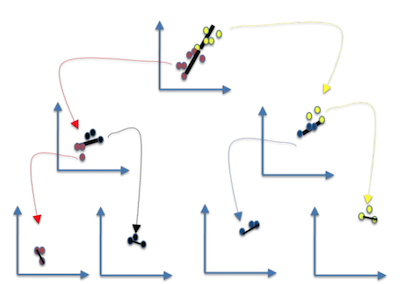
\includegraphics[height=3.6cm]{fig/fastmap.png}\hspace{1cm}
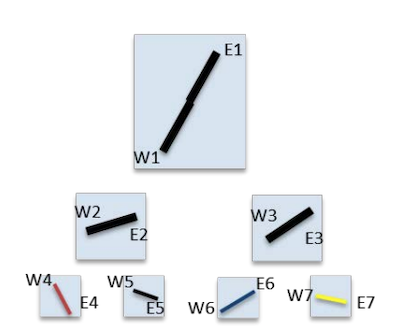
\includegraphics[height=3.6cm]{fig/tree1.png}
\end{center}

This tree of clusters was
generated via a recursive
  FASTMAP procedure~\cite{faloutsos1995fastmap}. Here, 
  $M$ is any example (selected at random).
  $E$  (east) is an example   furthest from $M$ and 
  $W$ (west) is an example   furthest from $E$.
  Note that $E,W$ can be found in time
  $O(2N)$.
  If  
  $c=dist(E,W)$ then
    other examples have distances $a,b$  to $E,W$, respectively and distance
    \mbox{ $x=(a^2+c^2-b^2) / (2c)$}
    on a line from  $E$ to $W$.
  By
splitting   data on   median $x$,
the examples can be then bi-clustered.
After generating the leaf clusters,
we can  (i)~evaluate just the centroid of each cluster;
then (ii)~propagating that label to all other items in that leaf.

As to other SSL approaches,
 {\em self training} algorithms~\cite{Yarowsky}  incrementally
guesses new labels from a learner
trained on all labels  seen to date.
Further, {\em GMM with expectation-maximization} algorithms~\cite{jonathonGMM}
use a Gaussian mixture
model to cluster the data (and use those clusters to label the data).
Furthermore,
 {\em label propagation algorithms}~\cite{Zhu02learningfrom} guess
labels using a majority vote across the labels  seen in nearby examples (or clusters).
Label propagation algorithms never update their old labels.
 {\em Label spreading} algorithms~\cite{Zhou04}, on the other hand,
update old labels using with feedback from subsequent labelling.
Label  spreading algorithm iterates on a similarity matrix
between example and   normalizes the edge weights by computing the normalized graph
of the Laplacian.\\\hline
\end{tabular}
\end{table} 


\subsection{Research Goal4:  get our recommendations used by CSS community}\label{goal4}

All the above work is pointless unless we can convince the
CSS community to use our results. In this regard, 
our experience offers much hope that these results
will be widely adopted. What we found is that if we go to projects with lists of problems and proposed improvements from that project,
then we find a ready audience. For example:
\bi
\item See the work documented in Table~\ref{casestudy};
\item We spend 2021 in bi-weekly meetings with the Linux kernel
team, discussing how our data mining results can improve their code.
\ei
In our experience, the only thing stopping the widespread
adoption of our prior results was the COVID crisis (that forced
many teams into working less with other teams and more with their
own internal workers). For the period 2022-2025 we anticipate far fewer problems with
COVID and much more collaboration between CSSI teams.


In any case, it will be important to track the application of these results. Hence:

\textcolor{red}{{\bf Measurable Outcomes:}} We will   log all our interactions with CSSI projects. We foresee that these interactions
will take three forms: (a)~initial tentative contacts;
(b)~preliminary results; (c)~review of impact, 12 months later.
We would say that {\bf Goal4} is achieved if our contacts is effective and frequent:
\bi
\item By ``frequent'', we are aiming for a least one tentative contact per month and four sets of preliminary results per year.
\item By ``effective'', we would use the same measurable outcomes
as seen in {\bf Goal3}.
\ei


\subsection{Research Goal5:  apply our methods to  CSS projects not stored in Github}\label{goal5}

For most of this project, we have assumed using data
from Github. But not all projects are stored in the location.
hence we need to check of our methods work for data from other venues.

We view {\bf Goal5} as being 
strongly connected to {\bf Goal4}. As a side-effect of all
the interactions associated with that goal, we will find
examples of code that is stored in locations other than Github.

What happens after that depends on the nature of those other sources:
\bi
\item
If these other locations support large scale data access
via web-based methods, we anticipate that our tools will readily transfer to other venues.
\item
Otherwise, we may be unable to achieve this goal.
\ei
In any case, it is important to track this issue:


\textcolor{red}{{\bf Measurable Outcomes:}} We will log all the non-Github sources found as part of this work. Also,
we will   log when (or if) our tools can achieve {\bf Goals1,2,3,4}.


\subsection{Research Goal6:  demonstrate that there exists a set of general methods   for improving CSS projects}\label{goal6}


Ideally, science can produce general
conclusions that hold in multiple contexts.
By that measure, how much of the above 
is ``scientifiic''? 

To say that another way,
what is the external validity of the conclusions reached
via the above methods? If we studied (say) 700 CSS projects, would we find general principles that hold across all these projects?
Or are all CSS projects are fundamentally different and nothing
can be generalized from one project to another?

 Before answering these quetions, we first motivate {\em why} they are worthy of discussion.
 If we could find a small number of models that represent the rest then that would have several benefits:
\bi
\item {\bf Training newcomers:} new CSS developers could be initiated by getting them to study the factors leading to CSS  project success or failure.
\item {\bf Tool development:} new tool development for CSS software could be focused
on the issues that our models find are most prevalent and most important for mitigating unhealthy project.
\item 
{\bf Early code quality improvement:} Suppose the year is 2026 and   this proposal found how CSS projects divide into communities. Suppose further
that the methods of this proposal have found quality predictors and effective plans for each of those communities. Now, new CSS
projects could quickly find the predictors and improvement plans most relevant to them {\em without running any of the tools of this project}just by (a)~finding its community; then (b)~looking up the predictors and plan known to work in that community.  
\ei
But what is the pragmatic reality about the probability of   general principles for 
improving CSS software?
Given the diversity of CSS systems, it seems unrealistic to believe that some single model holds for all projects. 
But if we cannot learn single models (for predicting project success) across all CSS projects, then perhaps we can find communities of projects with similar properties. If so, then to
reason about some new project, we need only know what ``community''the new project belongs to (after which, we can apply lessons learned from current members of that community).

Technically speaking, {\bf Goal6} is a 
{\em transfer learning task}~\cite{KrishnaMF16,Nam13,Ma2012,jing15,Kocaguneli2014,yu2017feature,jamshidi2017transfer,pan2009survey,qing2015cross,li2018cost};
i.e. what lessons about one kind of project can be transferred
to another.  To the best of our knowledge,
the transfer of knowledge (about predictors and plans for project success or failure) has not been previous explored for CSS code.
There are many reasons for using transfer learning.  Transfer learning can be useful when there is insufficient local data. Clark and Madachy~\cite{clark15} in their study of 65 software under-development by the US Defense Department in 2015 showed developers working in an uncommon area often benefit from transferring knowledge from more common areas.

One way to characterize transfer learning
methods
is the approach that it follows.  Firstly, {\em dimensional transformation} methods   manipulate the raw source data until it matches the target. An initial attempt on performing transfer learning with Dimensionality transform was undertaken by Ma et al.~\cite{Ma2012} with an algorithm called transfer naive Bayes (TNB). Since then there are many such algorithms have been proposed such as TCA~\cite{Nam13}, TCA+~\cite{Nam2015}, TPTL~\cite{liu2019two}, and balanced distribution~\cite{xu2019cross} (just to name a few).


Secondly, there is another group of algorithms invented by   PI Menzies
and his student Rahul
Krishna. According to the Oxford English Dictionary, the bellwether is the leading sheep of a flock, with a bell on its neck, that all other sheep follow.
A {\em bellwether} method~\cite{krishna2017simpler,krishna16}.
assumes that within a community of software projects, there is one exemplary project called the {\em bellwether}, which can define predictors for the others. This effect is called {\em the bellwether effect}. They exploit this Bellwether effect in their {\em  bellwether method}  that searches for such an exemplar bellwether project to construct a transfer learner with it. This proposal
will use the bellwether method since our experiments shows
that it out-performs dimensionality transform methods~\cite{krishna2017simpler}.

One problem with Krishna's bellwether methods is that the algorithm requires  an $O(N^2)$ comparison of all projects-- which becomes impractical when reasoning about (e.g.) 700 CSS projects~\cite{majumder2019learning}.  To solve that problem, 
PI Menzies and his student Suvodeep Majumder have added a clustering pre-processor to the bellwether method. In this approach, data from multiple projects is recursively grouped together into a
tree of clusters and sub-clusters and sub-sub-clusters etc.
The Bellwether method is applied to each leaf and the best model
is promoted up one level. Then at each level $i$ of the cluster tree,
 the bellwether method is applied to applied to all the models promoted up from level $i+1$.  The best model (as found by the bellwether method) is then promoted to level $i-1$.
 Promotion stops when the level $i$ performs worse
 than the models found at level $i+1$. In studies with  1,628 non CSS projects,
 this hierarchically bellwether method returns just six models; i.e. those 1628 projects could be approximated by by six communities (with one model from each community)~\cite{majumder2019learning}.
 


\textcolor{red}{{\bf Measurable Outcomes:}} In this project, we would repeat the Menzies \& Majumder hierarchical analysis
on CSS projects. {\bf Goal6} would be called a success if it could be shown that, for many $N$ CSS projects,  the
benefits seen in {\bf Goals,1,2,3,4,5} could be achieved via a small number of $M$ models 
($M \ll N$) models.


